\documentclass{tietreport}

% Import images
\usepackage[T1]{fontenc}
\usepackage{amsmath}
\usepackage{graphicx}
\usepackage{pdfpages}
% Rotate wide diagrams onto landscape pages
\usepackage{pdflscape}
% Keep each figure directly under its section heading
\usepackage{float}
% Tables and deployment diagram
\usepackage{booktabs}
\usepackage{array}
\usepackage{tikz}
\usetikzlibrary{positioning,arrows.meta,shapes.geometric,fit,backgrounds}

% Bibliography: written by hand (no biber needed), see end of document.

%% ==================================================
%% PROJECT FIELDS
%% ==================================================

\TitlePageHeader{%
  UCS503 - Software Engineering%
}

\ProjectTitle{%
  MediSynth%
}

\ProjectSubTitle{%
  A Hospital Management System with a
  Privacy-Preserving Synthetic Patient Data
  Engine (SynthetiX)%
}

\author{%
  \texttt{1024030787} Aryan Sharma \\
  \texttt{1024030792} Brahmdeep Singh Khanuja \\
  \texttt{1024030793} Keerat Singh Brar%
}

\TitlePageSubText{%
  Group: \texttt{3C55} BE Third Year, COE%
}

\AdvisorName{%
  Ms. Nisha Thakur%
}

\TitlePageFooterText{{%
    \large End-Semester Evaluation \\[0.2cm]
    \bfseries Computer Science and Engineering
    Department%
  } \\[0.15cm]
  Thapar Institute of Engineering and Technology,
  Patiala%
}

%% ==================================================

\begin{document}

\maketitle
\tableofcontents

% ===== CHAPTER 1: INTRODUCTION =====

\chapter{Introduction}

\section{Background and Context}

Hospital software teams increasingly need realistic patient data to build,
test, and demonstrate new systems before they can be deployed. This need
extends beyond production hospitals to academic and research settings, where
teams frequently have no legitimate way to access real patient records at
all. Real patient data is protected health information under regulations such
as HIPAA (United States) and India's Digital Personal Data Protection (DPDP)
Act, and cannot legally or ethically be shared with developers, students, or
third-party testers without extensive data-use agreements that are impractical
within a single academic semester.

MediSynth addresses this gap by pairing a fully functional, role-based
hospital management system (HMS) with Synthetix, a synthetic patient data
engine. Rather than relying on real records or simple field-masking,
Synthetix generates entirely new, artificial patient records that follow the
statistical patterns expected in real healthcare data---age--diagnosis
correlations, vital-sign and laboratory relationships, visit and admission
patterns---without representing any real individual. Access to these datasets
is itself governed: researchers must request a dataset, an administrator must
approve the request, and every preview and download is written to an audit
log.

\subsection{Problem Statement}

Student and early-stage development teams building healthcare software face
four related obstacles:

\begin{itemize}
  \item \textbf{Legal restriction:} real hospital records fall under HIPAA and
    the DPDP Act; hospitals cannot hand them to student developers or
    third-party testers without extensive data-use agreements that are
    impractical within a single semester.
  \item \textbf{Re-identification risk:} simple anonymization (removing names
    or ID numbers) is frequently reversible---prior research has shown that a
    large majority of a population can be uniquely re-identified from just
    three seemingly harmless fields such as date of birth, gender, and postal
    code \cite{sweeney2000}. This makes basic field-masking an unreliable
    substitute for genuine privacy protection.
  \item \textbf{Unrealistic test data:} teams that avoid real data often fall
    back on small, hand-typed mock records that do not reflect real clinical
    patterns, producing systems that are never properly stress-tested.
  \item \textbf{Fragmented development:} without a single, realistic, shared
    dataset, each part of a hospital system---backend, frontend,
    analytics---tends to invent its own inconsistent mock data, causing
    integration rework later in the project.
\end{itemize}

MediSynth's core engineering problem is therefore twofold: build a complete,
role-based hospital management system, and build a data engine that produces
statistically realistic, privacy-safe data together with a controlled way to
share it.

\section{Project Objectives}

\begin{enumerate}
  \item Deliver a role-based Hospital Management System with patient,
    doctor, lab technician, researcher and administrator roles, covering
    registration with administrator approval, appointment booking with slot
    conflict checking, doctor consultation, lab test workflows and audit
    logging, backed by a real PostgreSQL database.
  \item Design and implement Synthetix, a statistical synthetic-data
    generation engine that produces patient datasets of 500 to 50,000 records
    (reference size: 10,000) with zero real patient records, and an
    automatic evaluator that scores each dataset for fidelity, clinical
    relationships, validity and privacy before it may be released.
  \item Provide governed access to synthetic datasets: a dataset catalogue,
    request--approve--download workflow for researchers, immediate revocation
    when a dataset is retired, and an audit trail of every sensitive action.
\end{enumerate}

Objectives 1 and 3 are demonstrated end to end in the submitted code.
Objective 2 is measured in Chapter~\ref{ch:results}: datasets of 5,000 and
10,000 records pass every quality gate, while 500 and 2,000 records are
correctly rejected on privacy grounds.

\section{Scope and Project Status}

Table~\ref{tab:status} states plainly what is implemented against the
database and what is not yet connected, so that the evaluation is based on
the actual state of the system.

\begin{table}[H]
\centering
\small
\begin{tabular}{p{4.3cm}p{2.3cm}p{6.2cm}}
\toprule
\textbf{Feature} & \textbf{Status} & \textbf{Notes} \\
\midrule
Registration, login, JWT, roles & Implemented & Patients active at once; doctors, lab technicians and researchers wait for admin approval \\
Admin bootstrap and user control & Implemented & One-time bootstrap secret; suspend/reactivate users \\
Appointments & Implemented & 30-minute slots, conflict check, confirm/cancel/complete \\
Lab test workflow & Implemented & Order, start, complete; only the assigned technician may complete \\
Synthetic datasets (Synthetix) & Implemented & Generate, evaluate, regenerate, retire, preview, CSV download \\
Research access workflow & Implemented & Request, approve/reject, per-dataset access \\
Audit log & Implemented & Dataset and access events recorded \\
Prescriptions, pharmacy, billing & Frontend only & Screens run on demo data; no backend tables yet \\
Mobile application & Dropped & Out of scope for the final build \\
\bottomrule
\end{tabular}
\caption{Implementation status at the end-semester evaluation}
\label{tab:status}
\end{table}

% ===== CHAPTER 2: METHODOLOGY & DESIGN =====

\chapter{Methodology and Design}

\section{System Architecture}

\subsection{High-Level Design}

MediSynth is built as three coordinated parts sharing one PostgreSQL schema:

\begin{itemize}
  \item \textbf{Backend (Java 21, Spring Boot 4):} a stateless REST API
    (56 endpoints in 11 controllers) with JWT authentication and role-based
    access control. Layers follow the usual \texttt{controller $\rightarrow$
    service $\rightarrow$ repository $\rightarrow$ model} structure, with
    request and response DTOs and bean validation at the boundary.
  \item \textbf{Frontend (React 18, Vite):} the web interface with separate
    dashboards and navigation for patients, doctors, lab technicians,
    researchers and administrators.
  \item \textbf{Synthetix engine:} a pure-Java package
    (\texttt{com.personal.medisynth.synthetix}) with no framework
    dependencies, so it can be unit-tested and run on its own. The backend
    service layer calls it, stores its output in PostgreSQL and enforces the
    dataset lifecycle and access rules around it.
\end{itemize}

The mid-semester design placed Synthetix in a separate Python service. For
the final build it was implemented in Java inside the backend instead: this
removes a deployment dependency and lets dataset generation, evaluation and
access control share one transaction boundary. The engine is isolated behind
its own package, so a Python or machine-learning generator could replace it
later without changing the API.

\subsection{Technical Stack}

\begin{itemize}
  \item \textbf{Languages and frameworks:} Java 21 with Spring Boot 4.1.1,
    Spring Security, Spring Data JPA (Hibernate), Jakarta Bean Validation;
    React 18 with Vite 5 and React Router 6.
  \item \textbf{Database:} PostgreSQL. The schema is owned by Flyway
    migrations V1--V3; Hibernate runs in \texttt{validate} mode, so it never
    alters tables. Bulk synthetic rows are written with JDBC batch inserts.
  \item \textbf{Security:} JWT bearer tokens (JJWT), BCrypt password hashing,
    CORS allow-list, request rate limiting.
  \item \textbf{Tools:} Maven wrapper, Docker Compose for PostgreSQL, Git and
    GitHub, Postman for API testing, draw.io for the UML and data-flow
    diagrams, JUnit and Spring Boot Test for automated tests.
  \item \textbf{Libraries (frontend):} lucide-react for icons and plain CSS
    for styling; HTTP calls use the browser \texttt{fetch} API through a
    single service layer.
\end{itemize}

\subsection{Security Design}

The security rules were fixed early and every module follows them:

\begin{itemize}
  \item \textbf{Role and status are decided by the server.} The role is
    never read from a request body or from a token claim; it is loaded from
    the database on each request, so suspending a user takes effect at once.
  \item \textbf{Approval before access.} Doctors, lab technicians and
    researchers register as \texttt{PENDING\_APPROVAL} and receive no token
    until an administrator approves them.
  \item \textbf{One-time admin bootstrap.} The first administrator can be
    created only with a secret stored in the server environment
    (\texttt{ADMIN\_BOOTSTRAP\_SECRET}); once an admin exists the endpoint
    refuses further attempts. No secret is ever placed in frontend code.
  \item \textbf{Ownership checks.} A patient who asks for another patient's
    appointment receives 404, not 403, so records cannot be probed.
  \item \textbf{Safe errors.} Every error has one JSON shape with a code;
    stack traces are never returned. Repeated login attempts are rate
    limited and answered with HTTP 429.
\end{itemize}

\subsection{Database Design}

Table~\ref{tab:tables} lists the 13 tables created by the Flyway migrations.
Foreign keys enforce, for example, that an appointment must have a patient
and a doctor, and a partial unique index allows only one pending or approved
access request per researcher and dataset.

\begin{table}[H]
\centering
\small
\begin{tabular}{p{3.2cm}p{9.6cm}}
\toprule
\textbf{Migration} & \textbf{Tables} \\
\midrule
V1 initial schema & \texttt{users}, \texttt{patient\_profiles}, \texttt{doctor\_profiles}, \texttt{registration\_requests}, \texttt{appointments}, \texttt{research\_access\_requests}, \texttt{audit\_logs}, \texttt{bootstrap\_state} \\
V2 lab and research roles & \texttt{lab\_technician\_profiles}, \texttt{researcher\_profiles}, \texttt{lab\_test\_requests} \\
V3 Synthetix & \texttt{synthetic\_datasets}, \texttt{synthetic\_patient\_records}; adds \texttt{dataset\_id} to research requests \\
\bottomrule
\end{tabular}
\caption{Database tables by migration}
\label{tab:tables}
\end{table}

\section{Implementation Details}

\subsection{Module 1: Accounts, Approval and Access Control}

Patients register and are active immediately. Doctors, lab technicians and
researchers submit a registration with their professional details (for
example specialization and licence number for a doctor) and receive a
reference number; an administrator reviews the request and approves or
rejects it. Login for a pending or rejected account is refused with a clear
message. Passwords must be 10--72 characters with at least one letter and one
digit and are stored as BCrypt hashes.

\subsection{Module 2: Appointments}

Patients list approved doctors and book a 30-minute slot. The service checks
the slot against existing bookings and returns HTTP 409 on conflict; the
database also enforces uniqueness so two simultaneous requests cannot both
succeed. A doctor confirms or completes an appointment, and either party may
cancel according to the allowed state changes (pending $\rightarrow$
confirmed $\rightarrow$ completed, or cancelled).

\subsection{Module 3: Laboratory Workflow}

For a confirmed appointment a doctor orders a lab test; the patient is taken
from the appointment rather than typed in. Lab technicians see a queue of
pending tests, start one (which assigns it to them) and complete it with a
result. A different technician who tries to complete the same test receives
HTTP 403 (\texttt{NOT\_YOUR\_TEST}). The patient then sees the result.

\subsection{Module 4: Synthetix Synthetic Data Engine}
\label{sec:synthetix}

\paragraph{Generation.} Synthetix is a seeded, rule-based causal sampler.
The same seed always reproduces the same dataset. Each synthetic patient is
drawn in dependency order:
\begin{enumerate}
  \item age band and gender from a \emph{source profile};
  \item BMI and smoking status, depending on age and gender;
  \item primary diagnosis, chosen from ten ICD-10 codes (Table~\ref{tab:icd})
    by a softmax over scores that depend on age, BMI and smoking;
  \item vital signs and laboratory values (blood pressure, heart rate,
    fasting glucose, HbA1c, haemoglobin, cholesterol, creatinine) shifted by
    the diagnosis;
  \item outpatient visits in the last year, admission, length of stay and
    outcome, driven by the diagnosis and its acuity.
\end{enumerate}
Ages of 90 and over are top-coded to 90, and identifiers are a shuffled
sequence (\texttt{SYN-0000001}, \dots) with no link to any real patient.

\begin{table}[H]
\centering
\small
\begin{tabular}{llll}
\toprule
\textbf{ICD-10} & \textbf{Condition} & \textbf{Chronic} & \textbf{Adults only} \\
\midrule
Z00 & Routine health check & no & no \\
J06 & Acute upper respiratory infection & no & no \\
M54 & Back pain & no & no \\
J45 & Asthma & yes & no \\
I10 & Essential hypertension & yes & yes \\
E11 & Type 2 diabetes mellitus & yes & yes \\
E78 & Hyperlipidaemia & yes & yes \\
I25 & Chronic ischaemic heart disease & yes & yes \\
J44 & Chronic obstructive pulmonary disease & yes & yes \\
N18 & Chronic kidney disease & yes & yes \\
\bottomrule
\end{tabular}
\caption{Diagnoses modelled by Synthetix}
\label{tab:icd}
\end{table}

\paragraph{Source profile.} The only information taken from real hospital
data is a grouped count of patients by ten-year age band and gender.
Groups with fewer than 5 patients are suppressed; if the hospital has fewer
than 50 patients the counts are ignored and built-in population priors are
used; otherwise the counts are blended with the priors (shrinkage of 50). No
row-level data ever reaches the generator.

\paragraph{Evaluation.} After generation every dataset is scored by an
evaluator. The overall score is
\[
  S = 0.35\,S_{\text{marginal}} + 0.20\,S_{\text{relationships}}
    + 0.15\,S_{\text{validity}} + 0.30\,S_{\text{privacy}},
\]
where $S_{\text{marginal}}$ compares each column's distribution with
reference values, $S_{\text{relationships}}$ is the share of eight clinical
checks that hold (for example diabetic patients have higher fasting glucose,
hypertensive patients higher systolic pressure, chronic conditions more
visits), $S_{\text{validity}}$ is the share of values inside plausible
ranges, and $S_{\text{privacy}}$ is based on $k$-anonymity with $k=5$ over
age band, gender and diagnosis \cite{sweeney2002}. A dataset is marked
\textsc{ready} only if all gates in Table~\ref{tab:gates} are met;
otherwise it is marked \textsc{needs regeneration} with the reasons listed.

\begin{table}[H]
\centering
\small
\begin{tabular}{lc}
\toprule
\textbf{Gate} & \textbf{Required} \\
\midrule
Overall score $S$ & $\ge 0.90$ \\
Validity & $\ge 0.999$ \\
Records in groups of at least 5 look-alikes & $\ge 95\%$ \\
Records unique on age band, gender, diagnosis & $\le 1\%$ \\
Duplicate rows & none \\
Clinical relationships preserved & $\ge 6$ of 8 \\
\bottomrule
\end{tabular}
\caption{Release gates applied by the evaluator}
\label{tab:gates}
\end{table}

\paragraph{Lifecycle.} A dataset is created in state \textsc{evaluating}.
Evaluation moves it to \textsc{ready} or \textsc{needs regeneration}.
Regeneration uses a new seed, increases the version number and returns the
dataset to \textsc{evaluating}. From any state an administrator may
\textsc{retire} it (State Diagram~3).

\subsection{Module 5: Governed Dataset Access}

A researcher browses the catalogue of \textsc{ready} datasets and requests
access to one; a free-text request is also accepted. Only an approved request
for that dataset allows a preview of the first rows or a CSV download.
Retiring a dataset ends all access immediately, and datasets that are not
\textsc{ready} are answered with 404. Duplicate pending or approved requests
are refused, and approving a request for a dataset that is no longer ready
returns 409. The CSV is fetched by the frontend with the bearer token and
saved as a file; the \texttt{Content-Disposition} header is exposed through
CORS for this purpose.

\subsection{Module 6: Audit Logging}

Dataset generation, evaluation, regeneration, retirement, preview and
download, together with access decisions, are written to the \texttt{audit\_logs}
table and shown to administrators.

\subsection{Module 7: Frontend}

The React application has route guards per role and a service layer in which
every function has a real (HTTP) and a mock (in-memory) implementation,
selected by one flag. With the flag off, which is the default, accounts,
approvals, appointments, lab tests, datasets and research requests all use
the backend. Prescription, pharmacy and billing screens still use demo data.

% ===== CHAPTER 3: DIAGRAMS (kept from the mid-semester report) =====

\chapter{Diagrams}
\label{ch:diagrams}

This chapter collects the UML and data-flow diagrams
that describe the MediSynth system: use cases, class
structure, workflows (activity and swimlane diagrams),
data flow, object interactions (sequence and
collaboration diagrams), object life cycles (state
diagrams), and the software components.

% ----- Use case -----
\section{Use Case Diagram}

\begin{figure}[H]
  \centering
  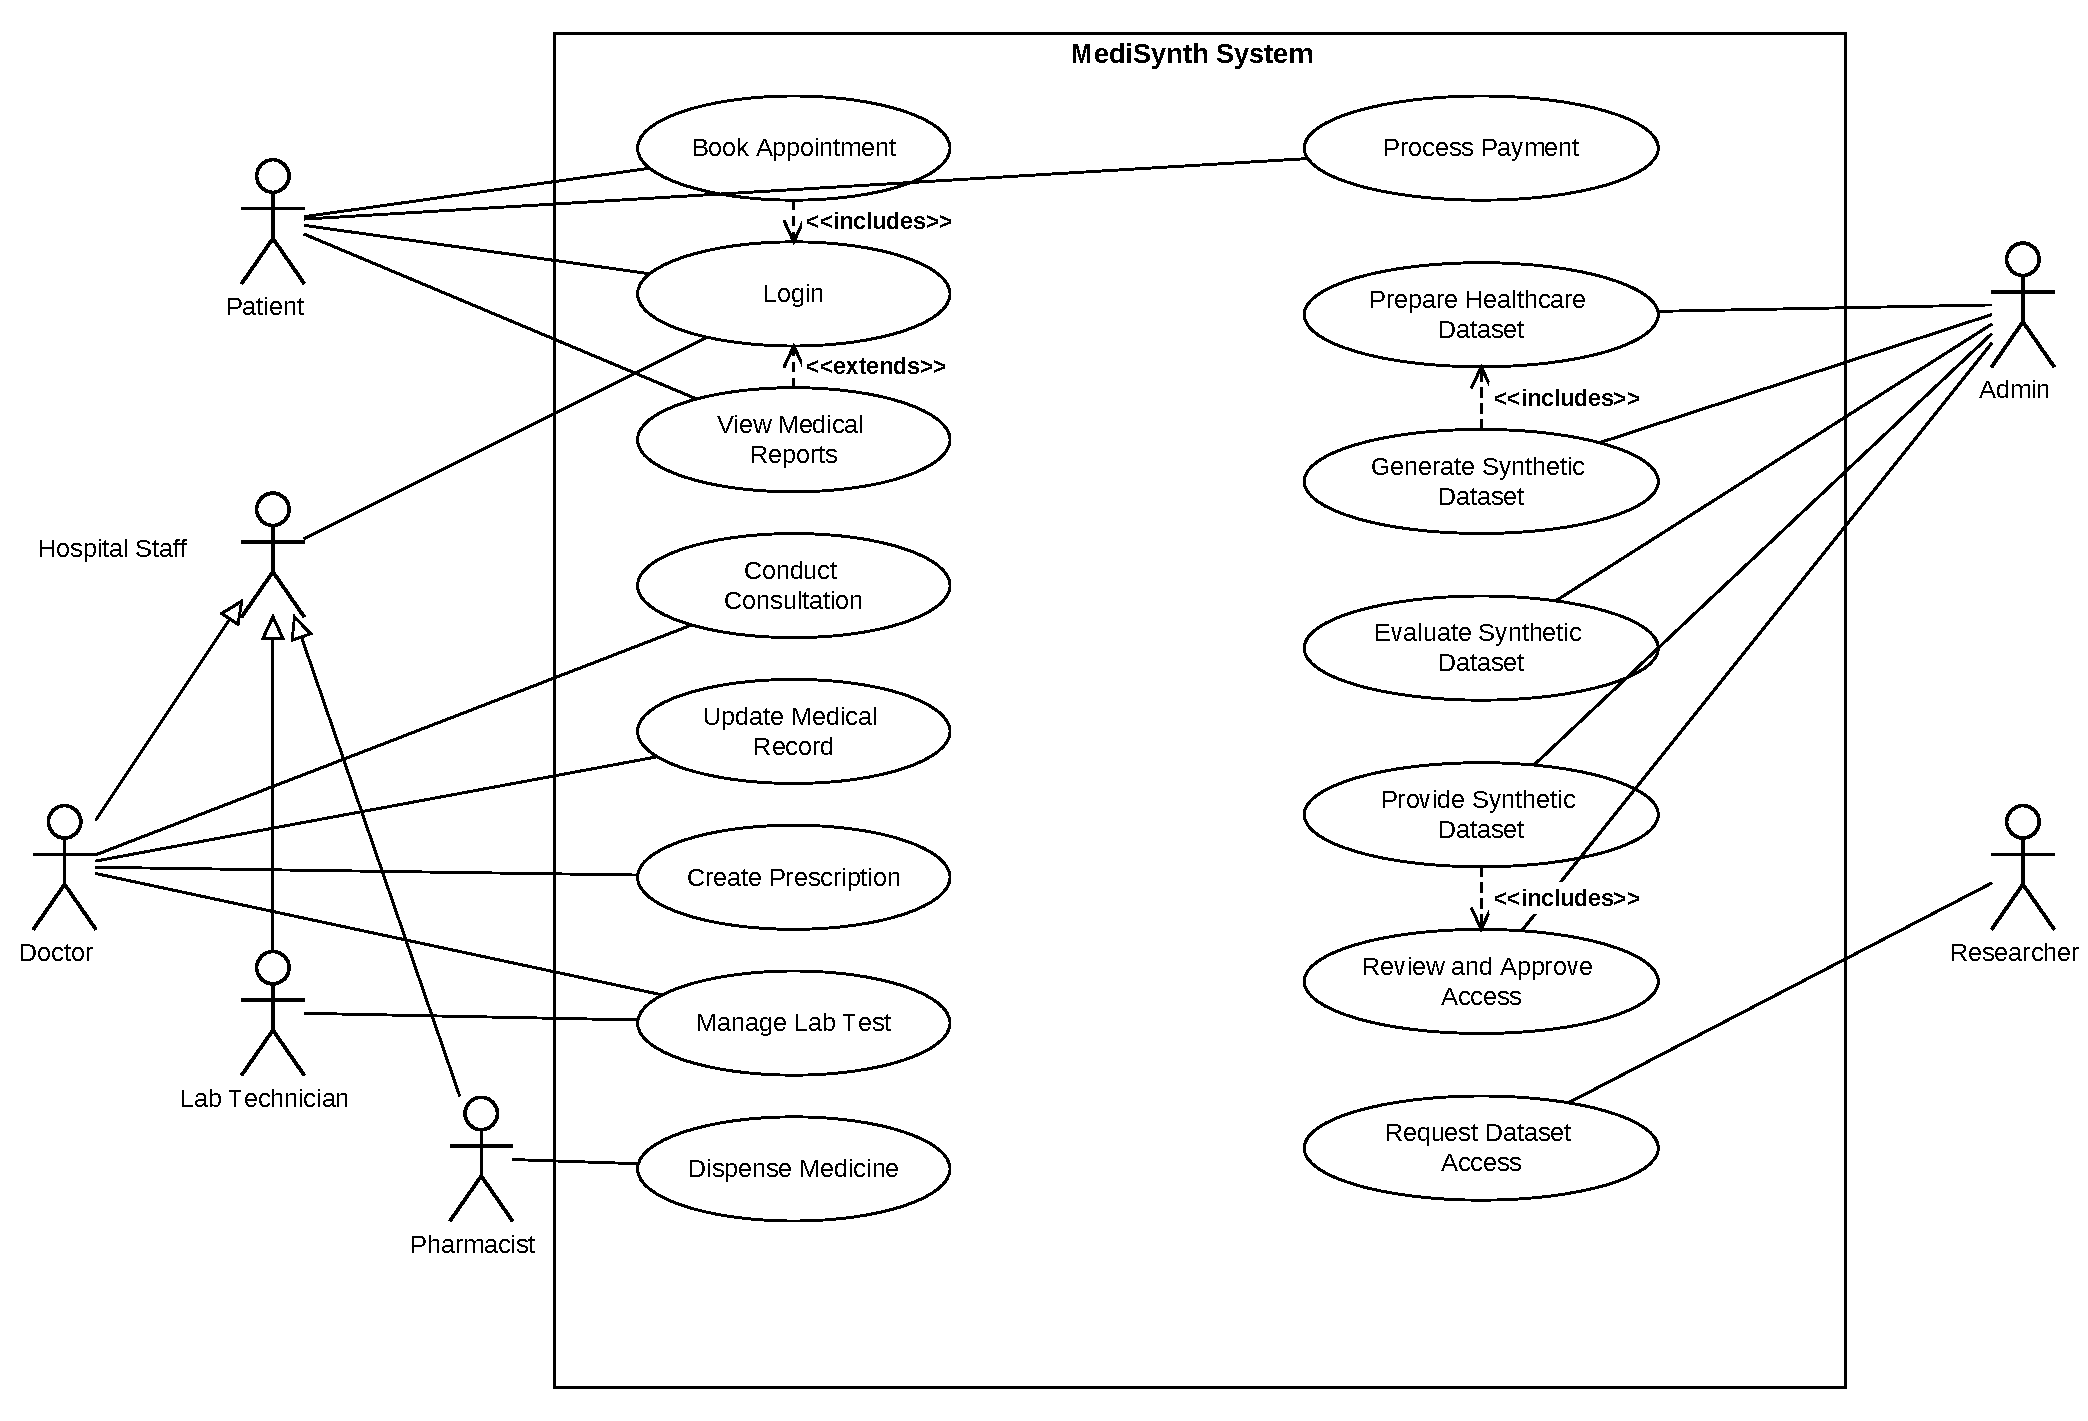
\includegraphics[width=\textwidth,height=0.72\textheight,keepaspectratio]{figures/usecase.pdf}
  \caption{Use case diagram for MediSynth}
  \label{fig:usecase}
\end{figure}
\clearpage

% ----- Class diagram -----
\begin{landscape}
\section{Class Diagram}
\begin{figure}[H]
  \centering
  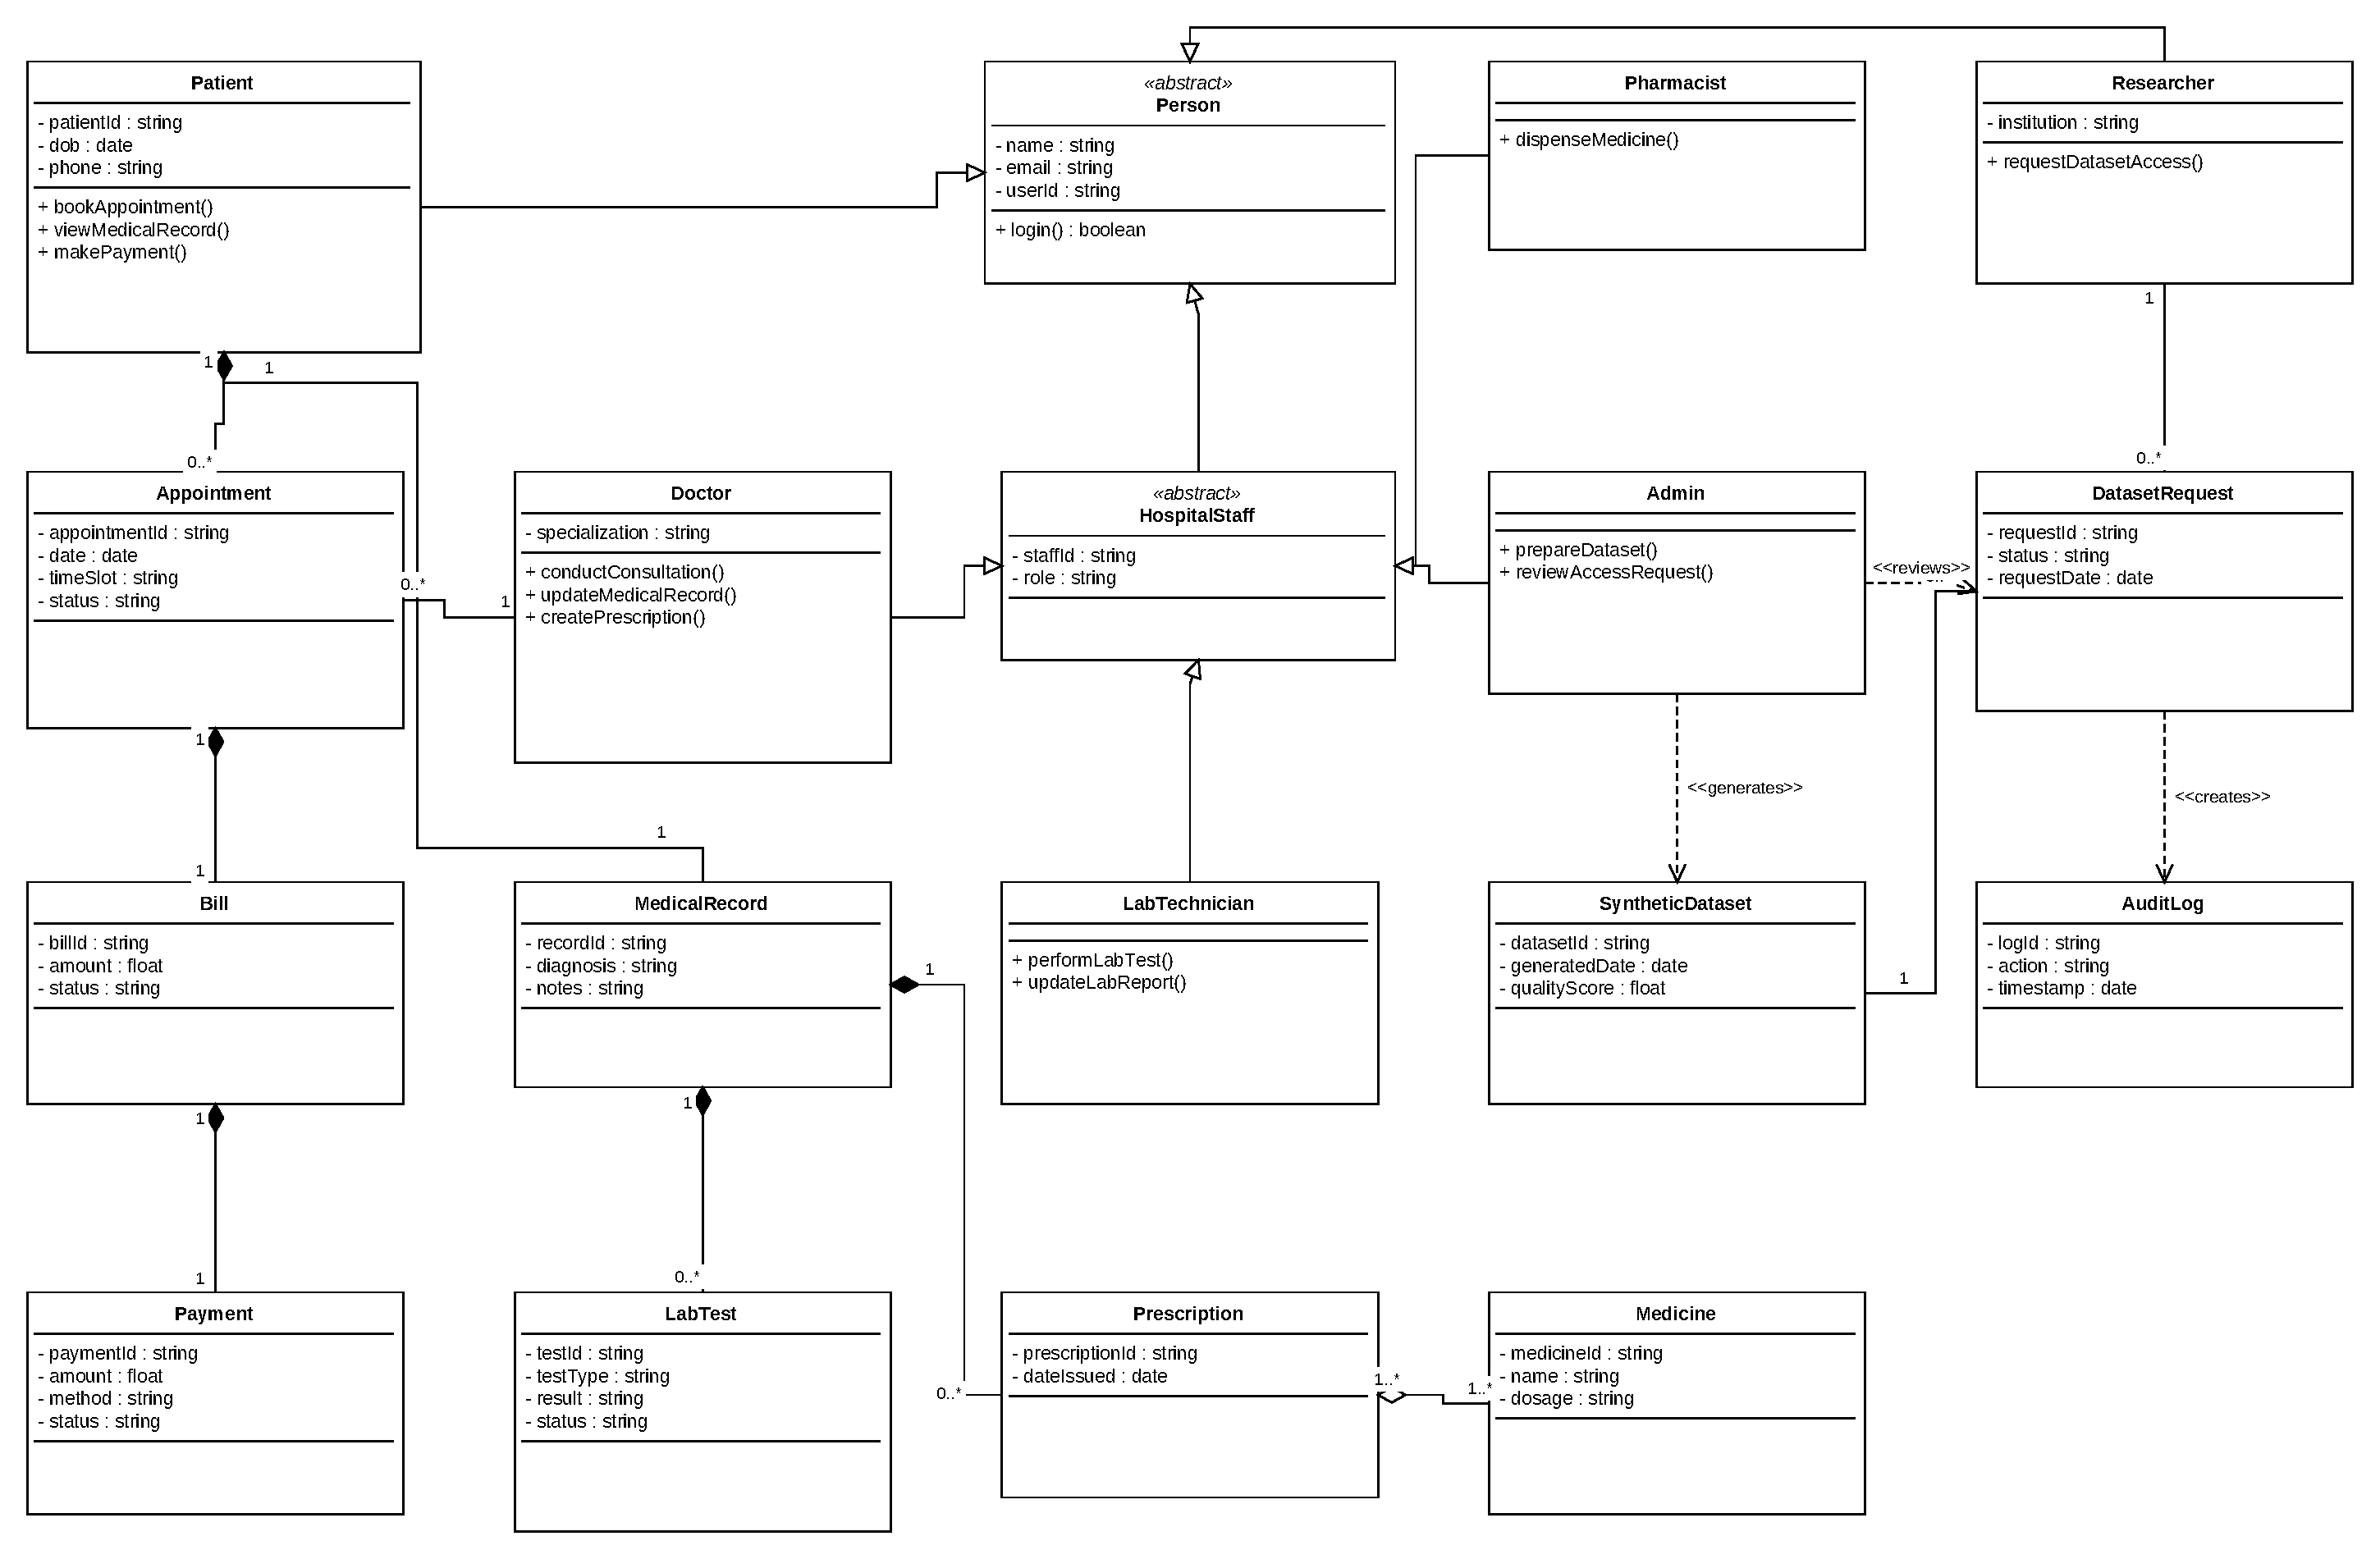
\includegraphics[width=\linewidth,height=0.82\textheight,keepaspectratio]{figures/class.pdf}
  \caption{Class diagram for MediSynth}
  \label{fig:class}
\end{figure}
\end{landscape}

% ----- Activity diagrams -----
\begin{landscape}
\section{Activity Diagram: Patient / Hospital Workflow}
\begin{figure}[H]
  \centering
  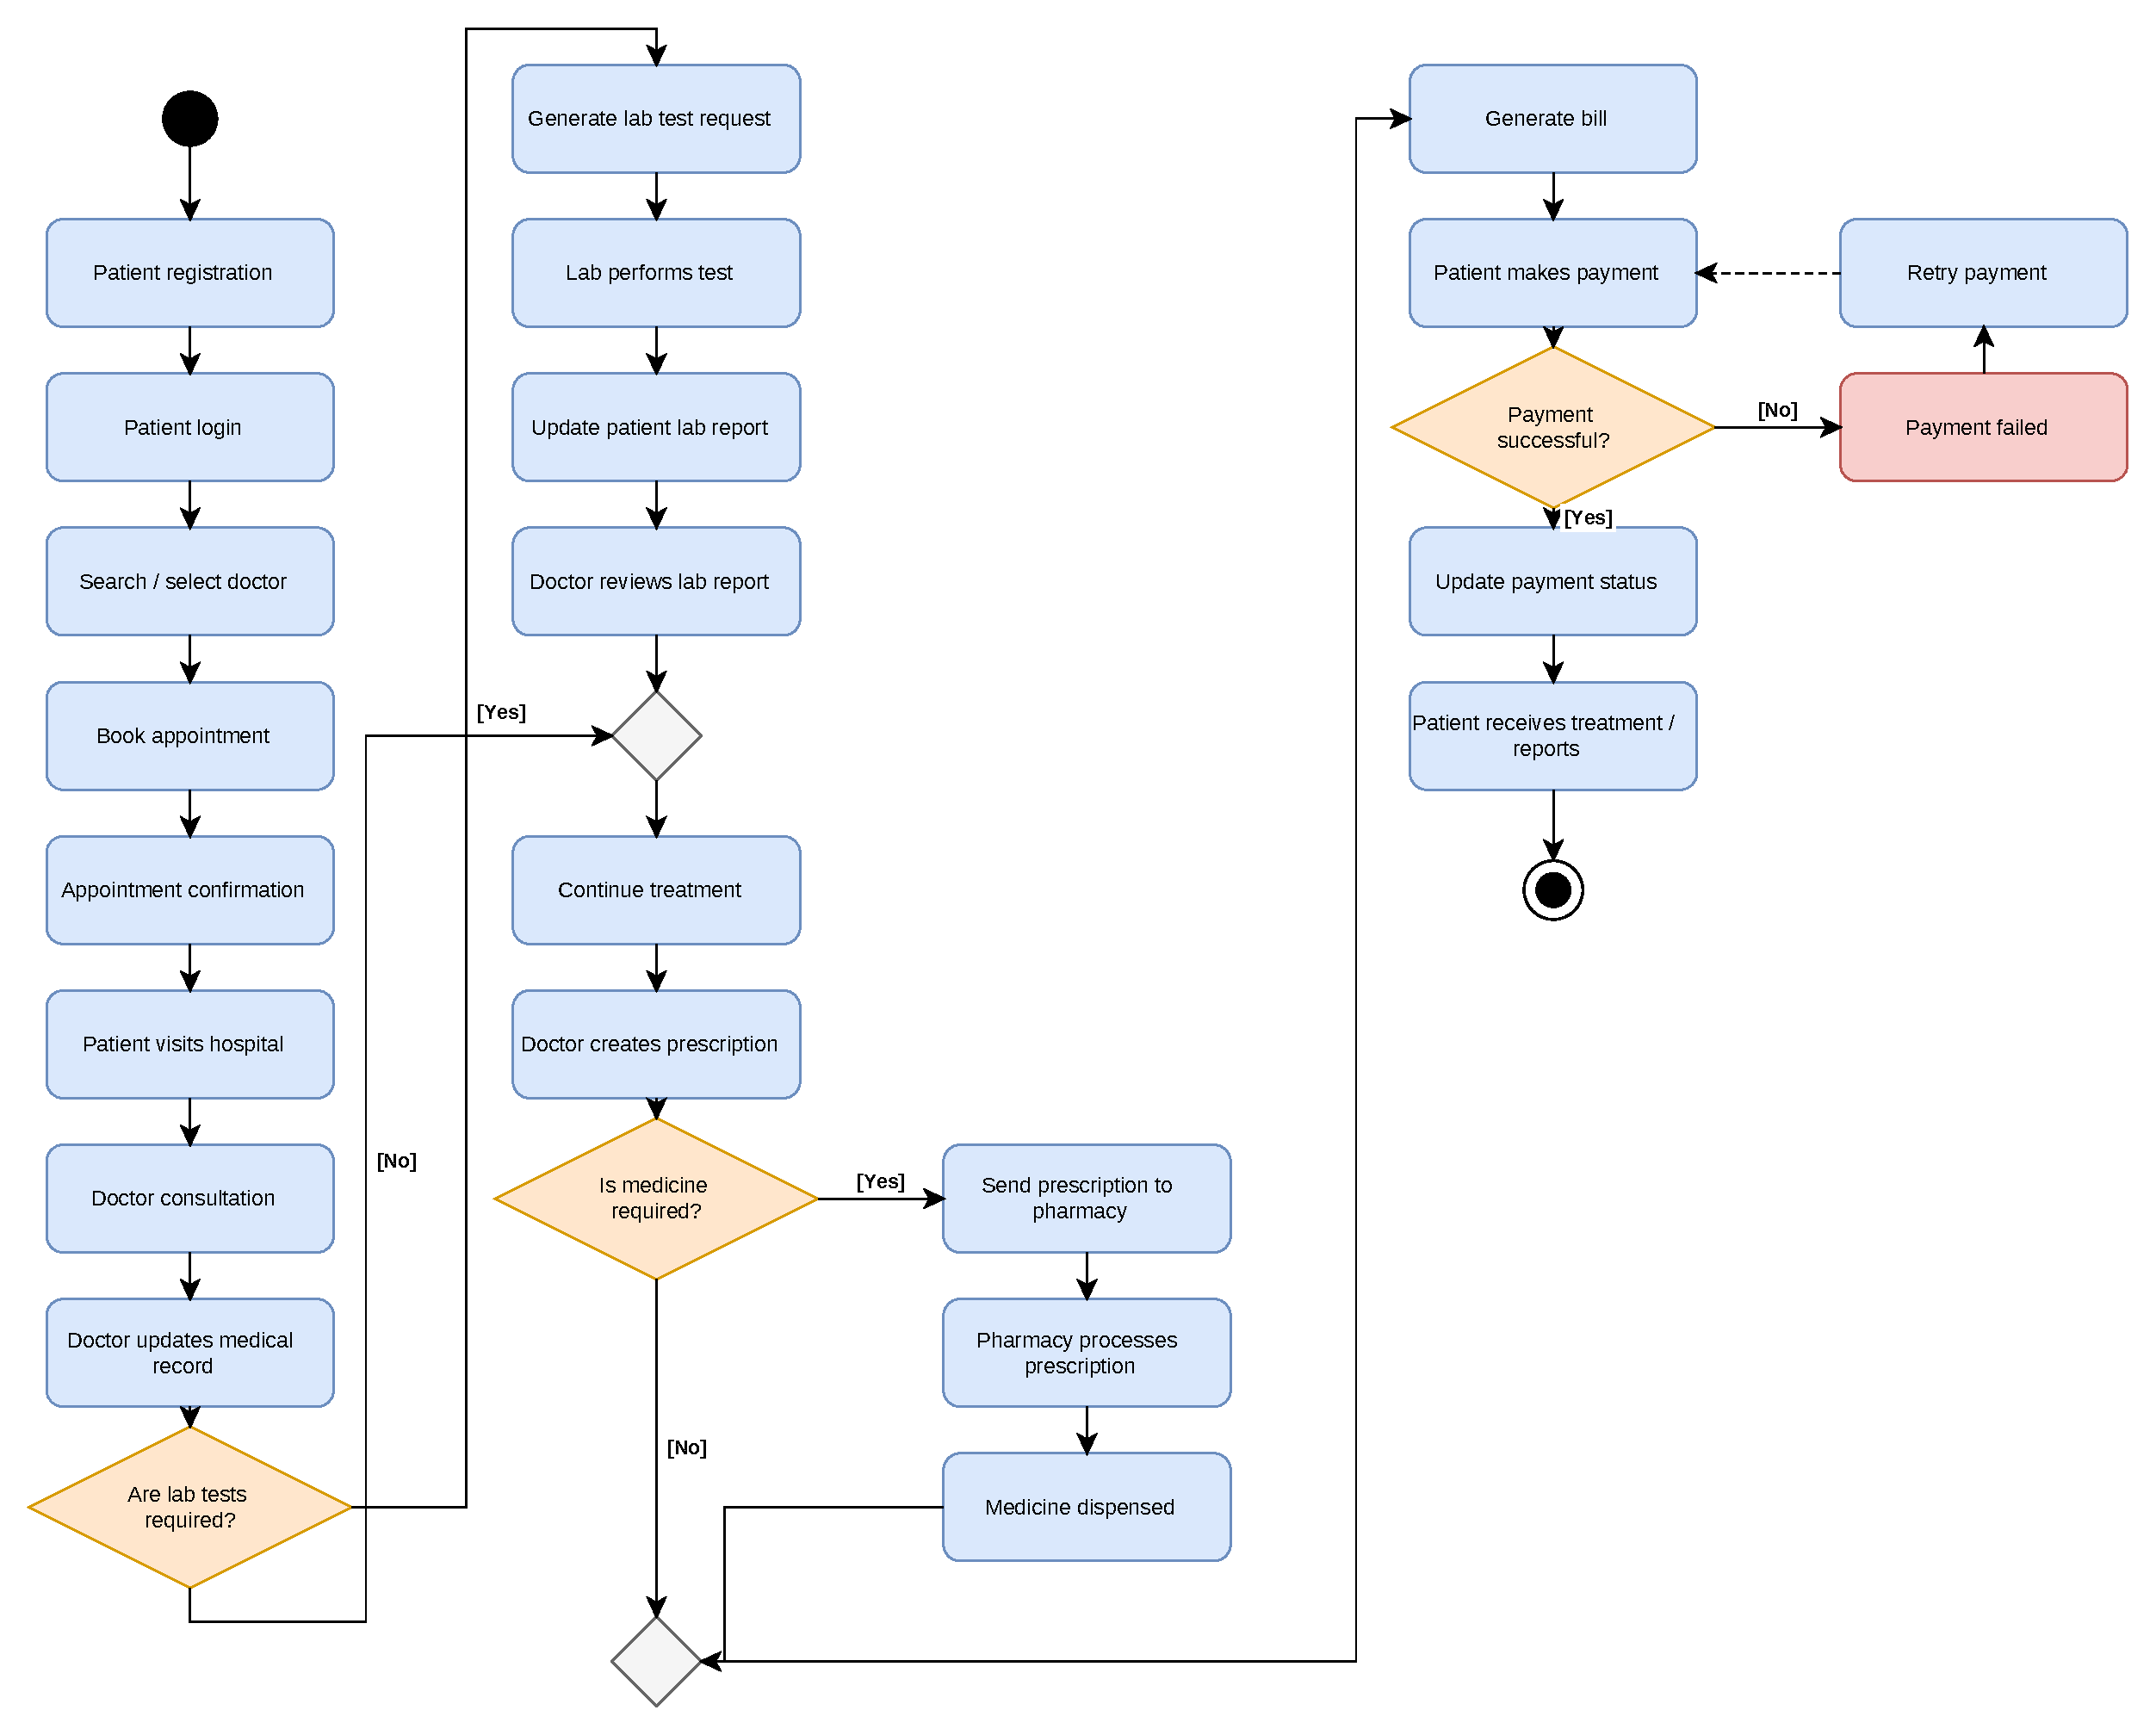
\includegraphics[width=\linewidth,height=0.82\textheight,keepaspectratio]{figures/activity1.pdf}
  \caption{Activity diagram: patient / hospital workflow}
  \label{fig:activity1}
\end{figure}
\end{landscape}

\section{Activity Diagram: Synthetix Workflow}

This workflow begins once sufficient patient / medical
record data has been accumulated by the hospital
workflow.

\begin{figure}[H]
  \centering
  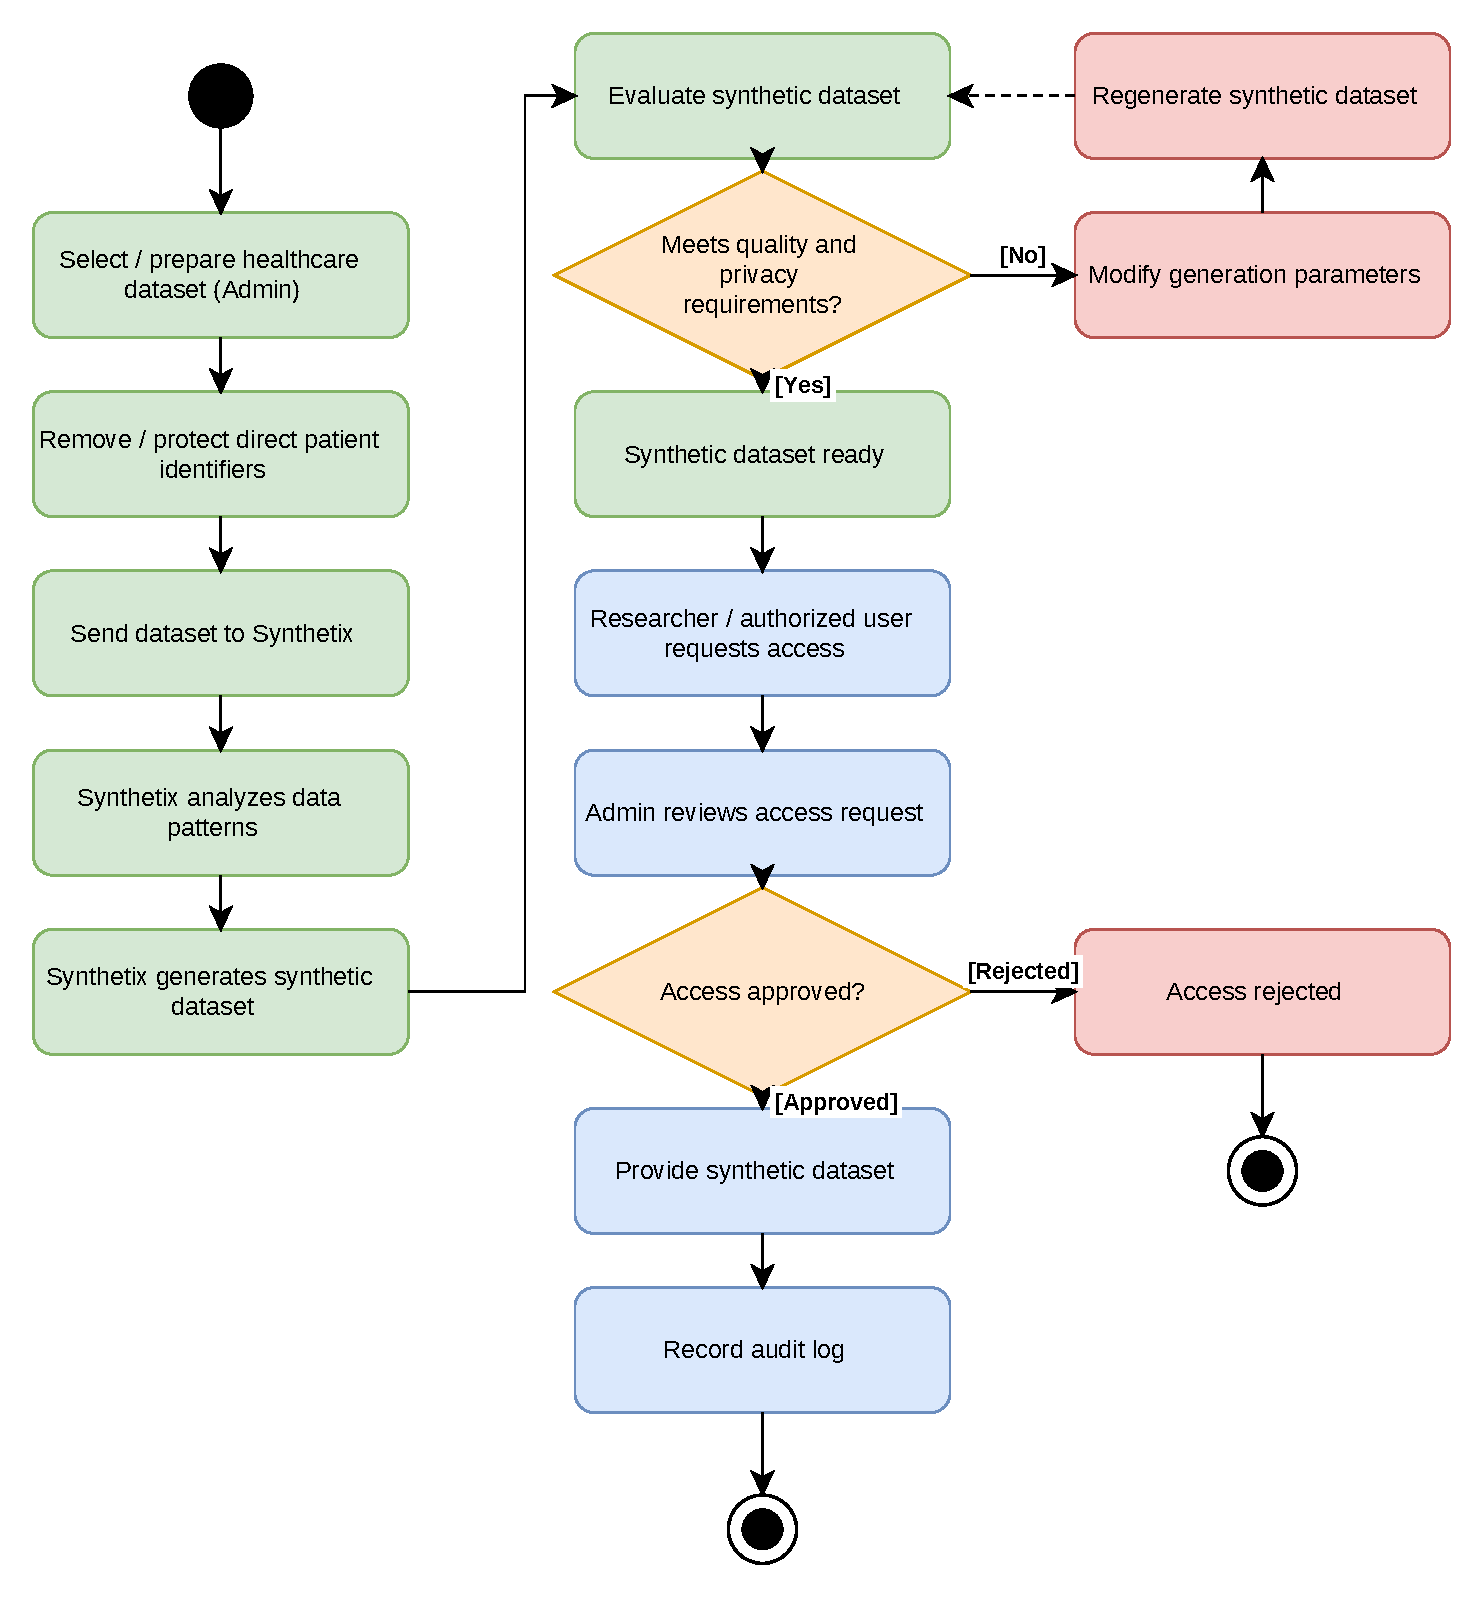
\includegraphics[width=\textwidth,height=0.66\textheight,keepaspectratio]{figures/activity2.pdf}
  \caption{Activity diagram: Synthetix workflow}
  \label{fig:activity2}
\end{figure}
\clearpage

% ----- Swimlane diagrams -----
\section{Swimlane Diagram 1: Patient / Hospital Workflow}

\begin{figure}[H]
  \centering
  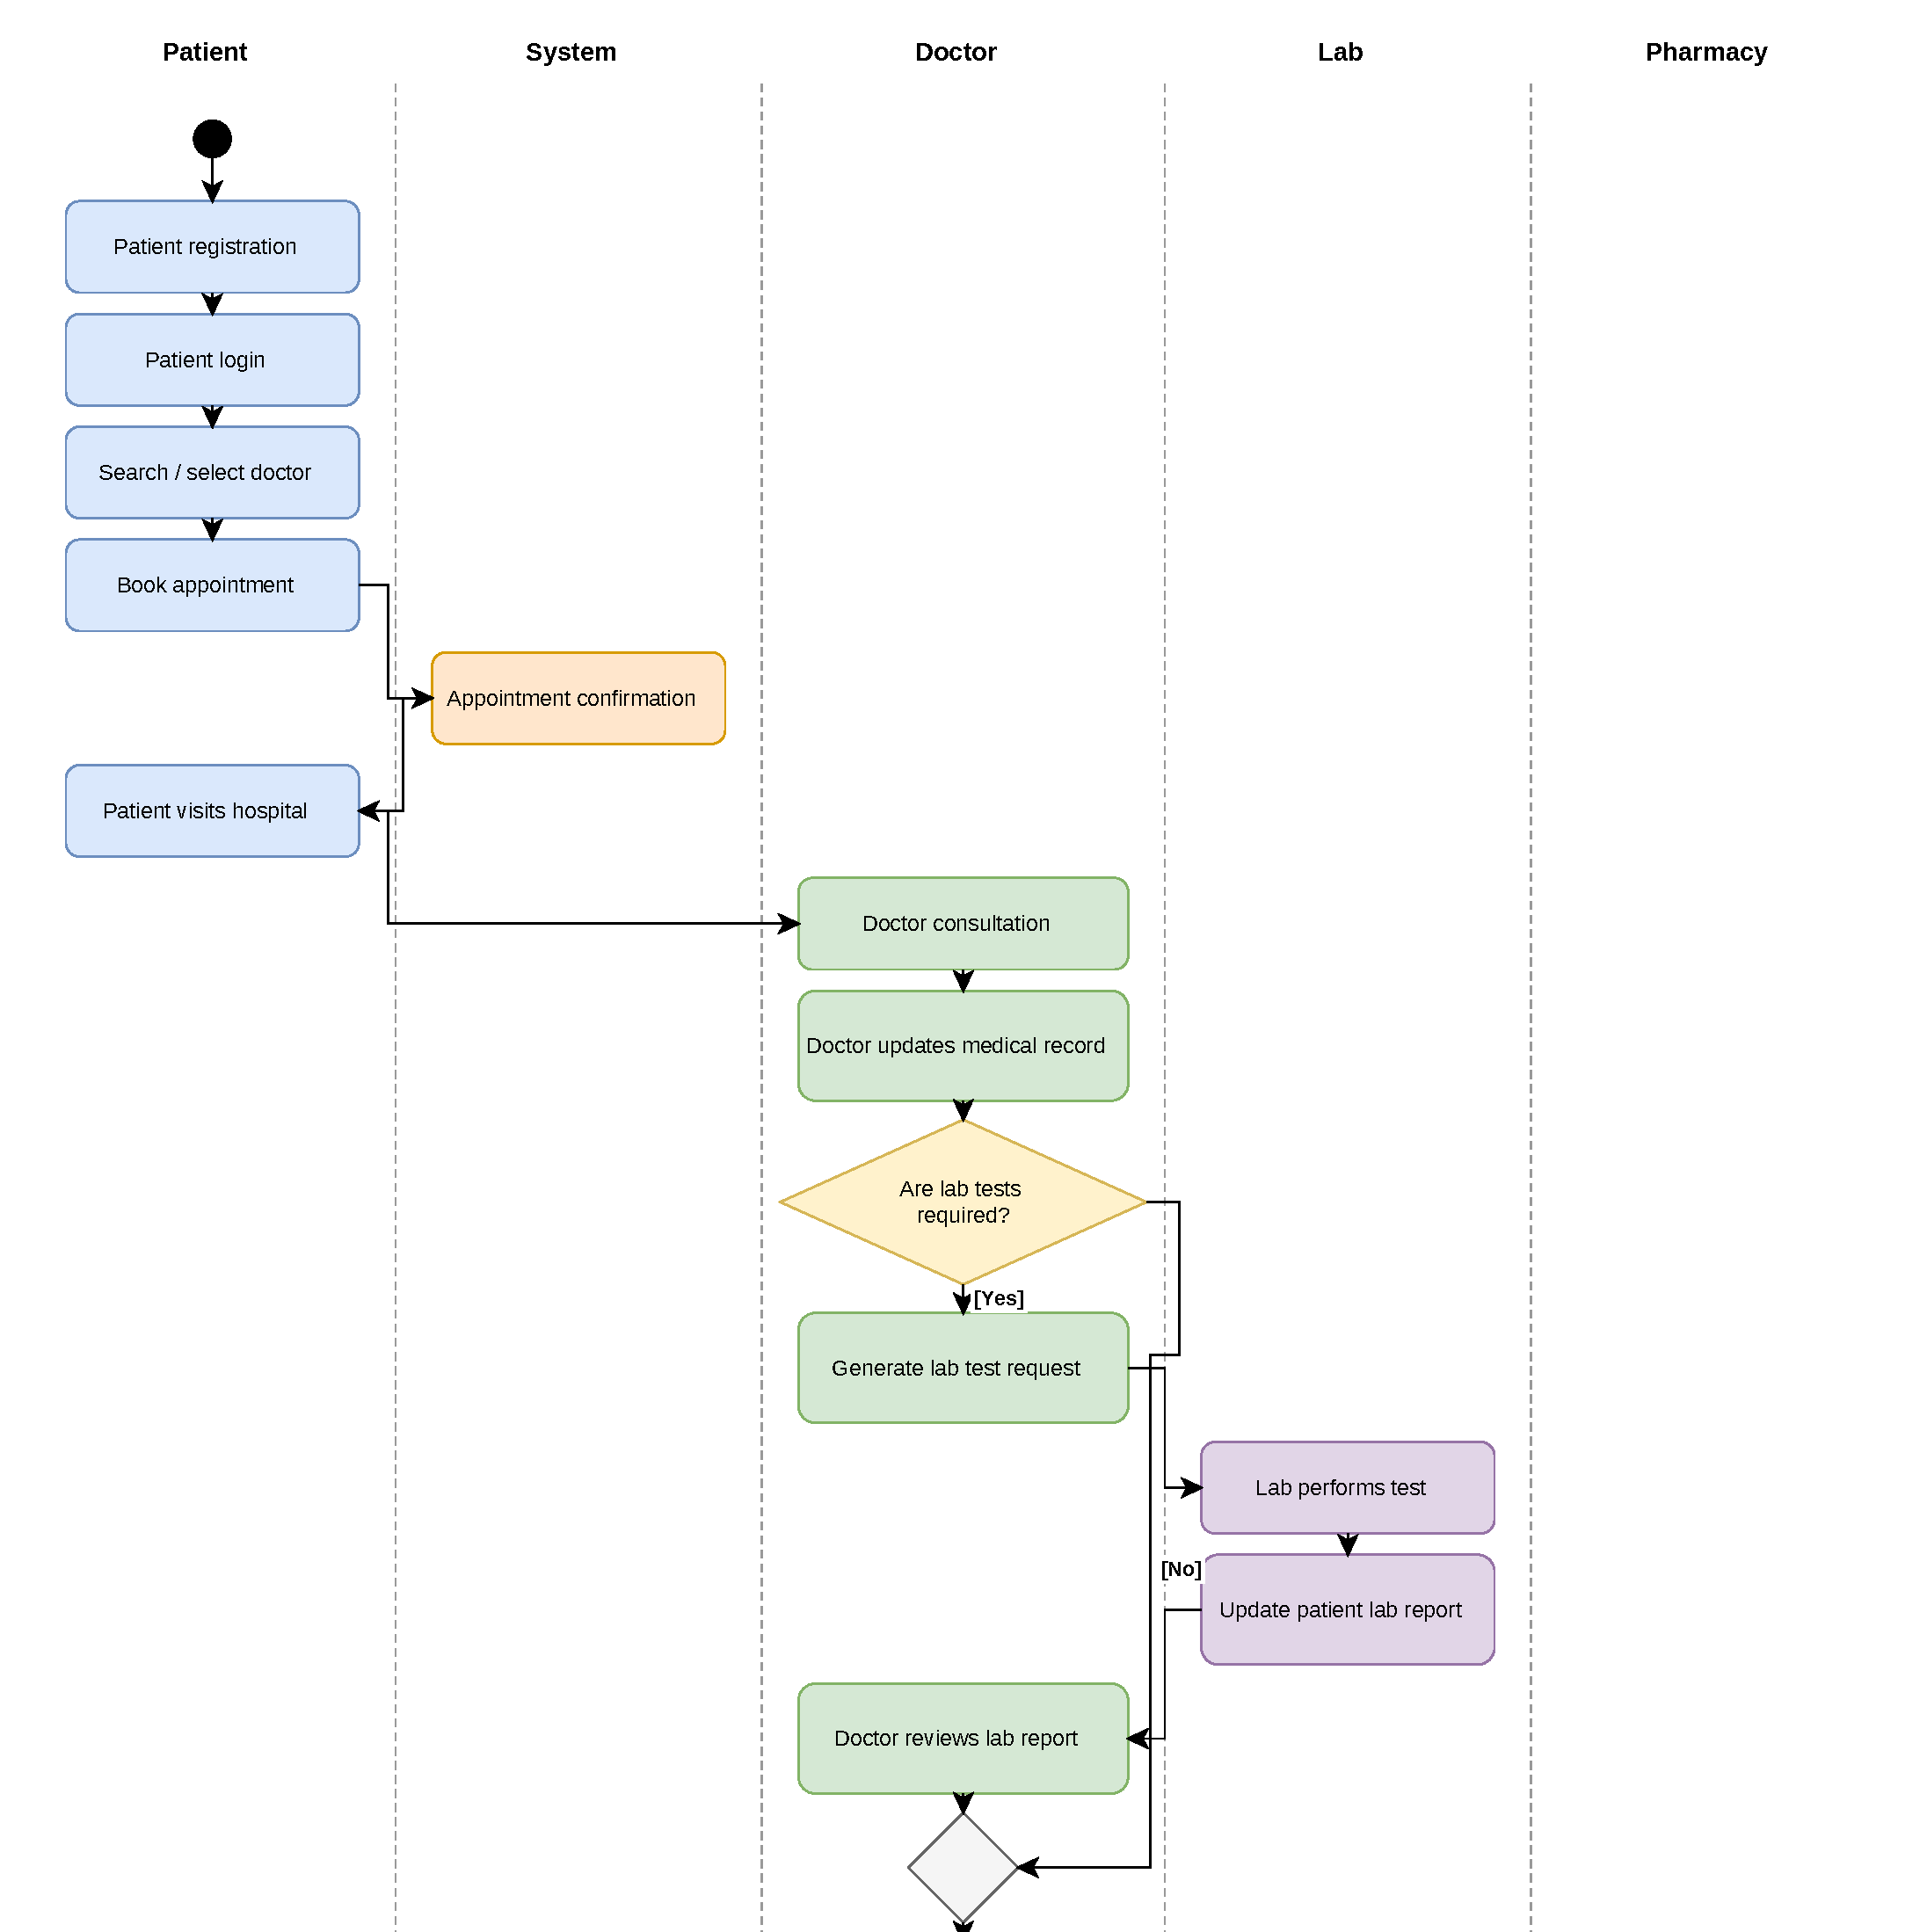
\includegraphics[width=\textwidth,height=0.72\textheight,keepaspectratio]{figures/swimlane1a.pdf}
  \caption{Swimlane diagram 1: patient / hospital workflow (part 1)}
  \label{fig:swimlane1a}
\end{figure}
\clearpage

\begin{figure}[H]
  \centering
  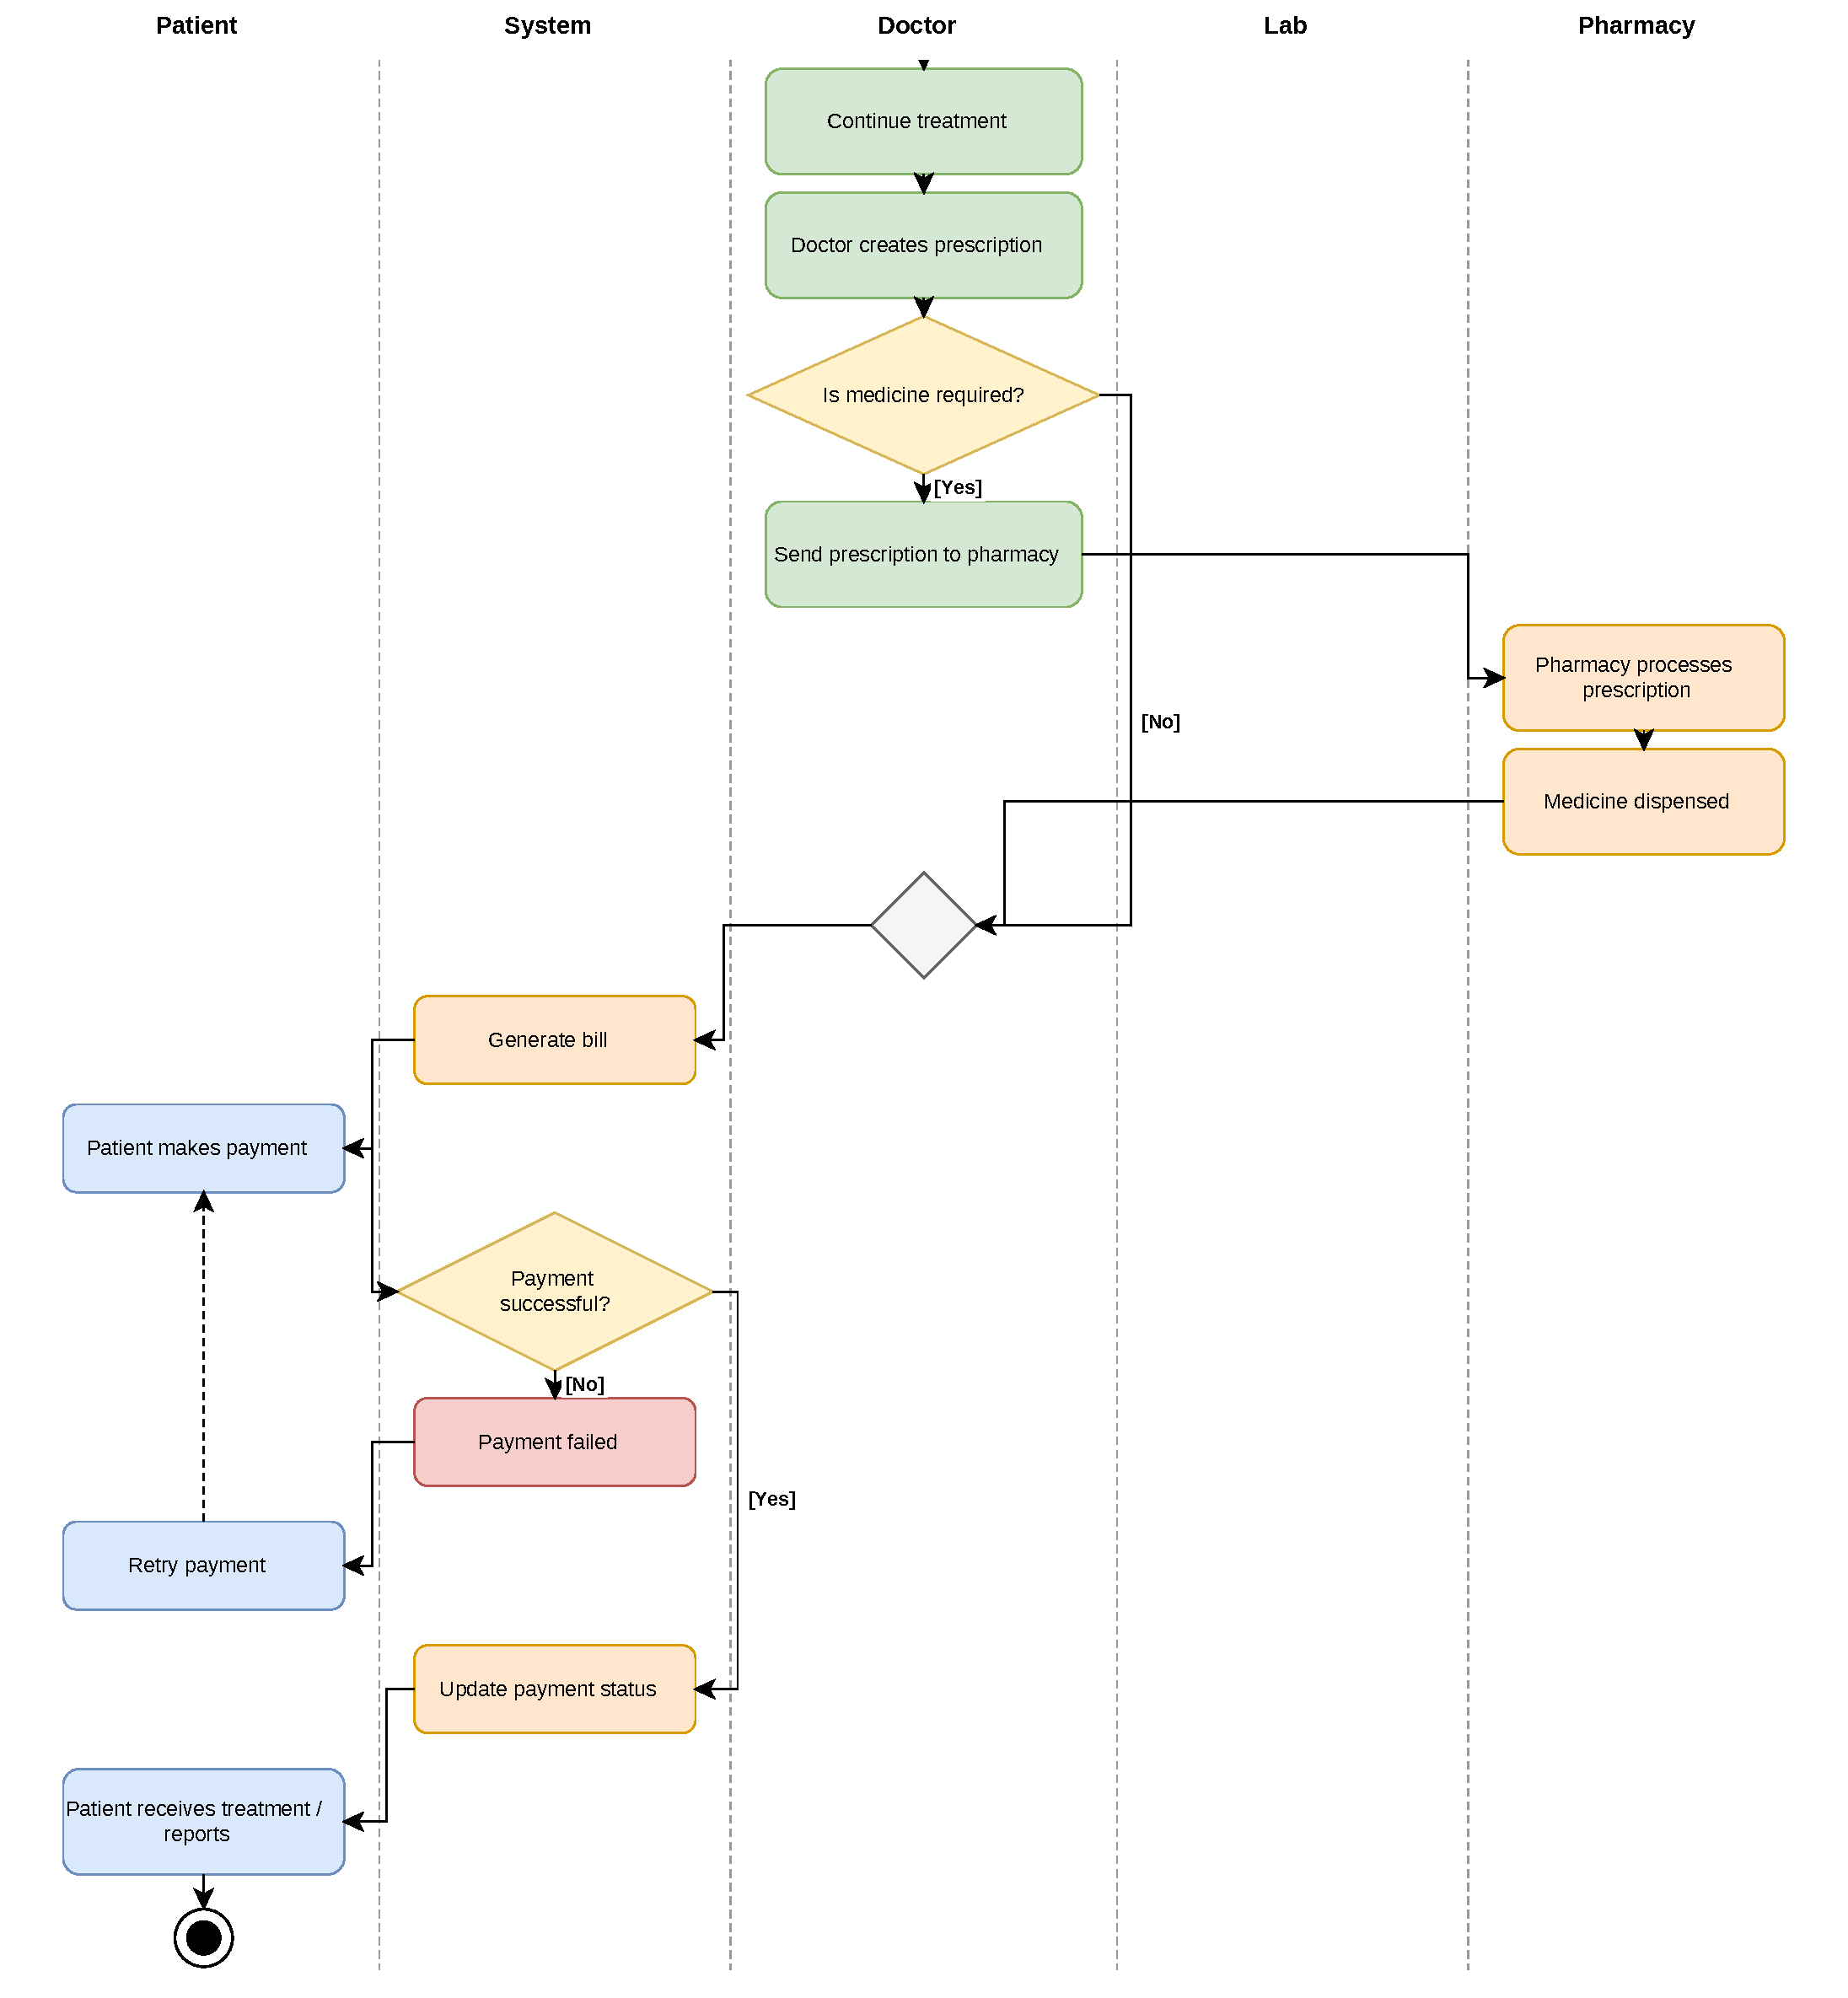
\includegraphics[width=\textwidth,height=0.72\textheight,keepaspectratio]{figures/swimlane1b.pdf}
  \caption{Swimlane diagram 1: patient / hospital workflow (part 2, continued)}
  \label{fig:swimlane1b}
\end{figure}
\clearpage

\section{Swimlane Diagram 2: Synthetix Workflow}

\begin{figure}[H]
  \centering
  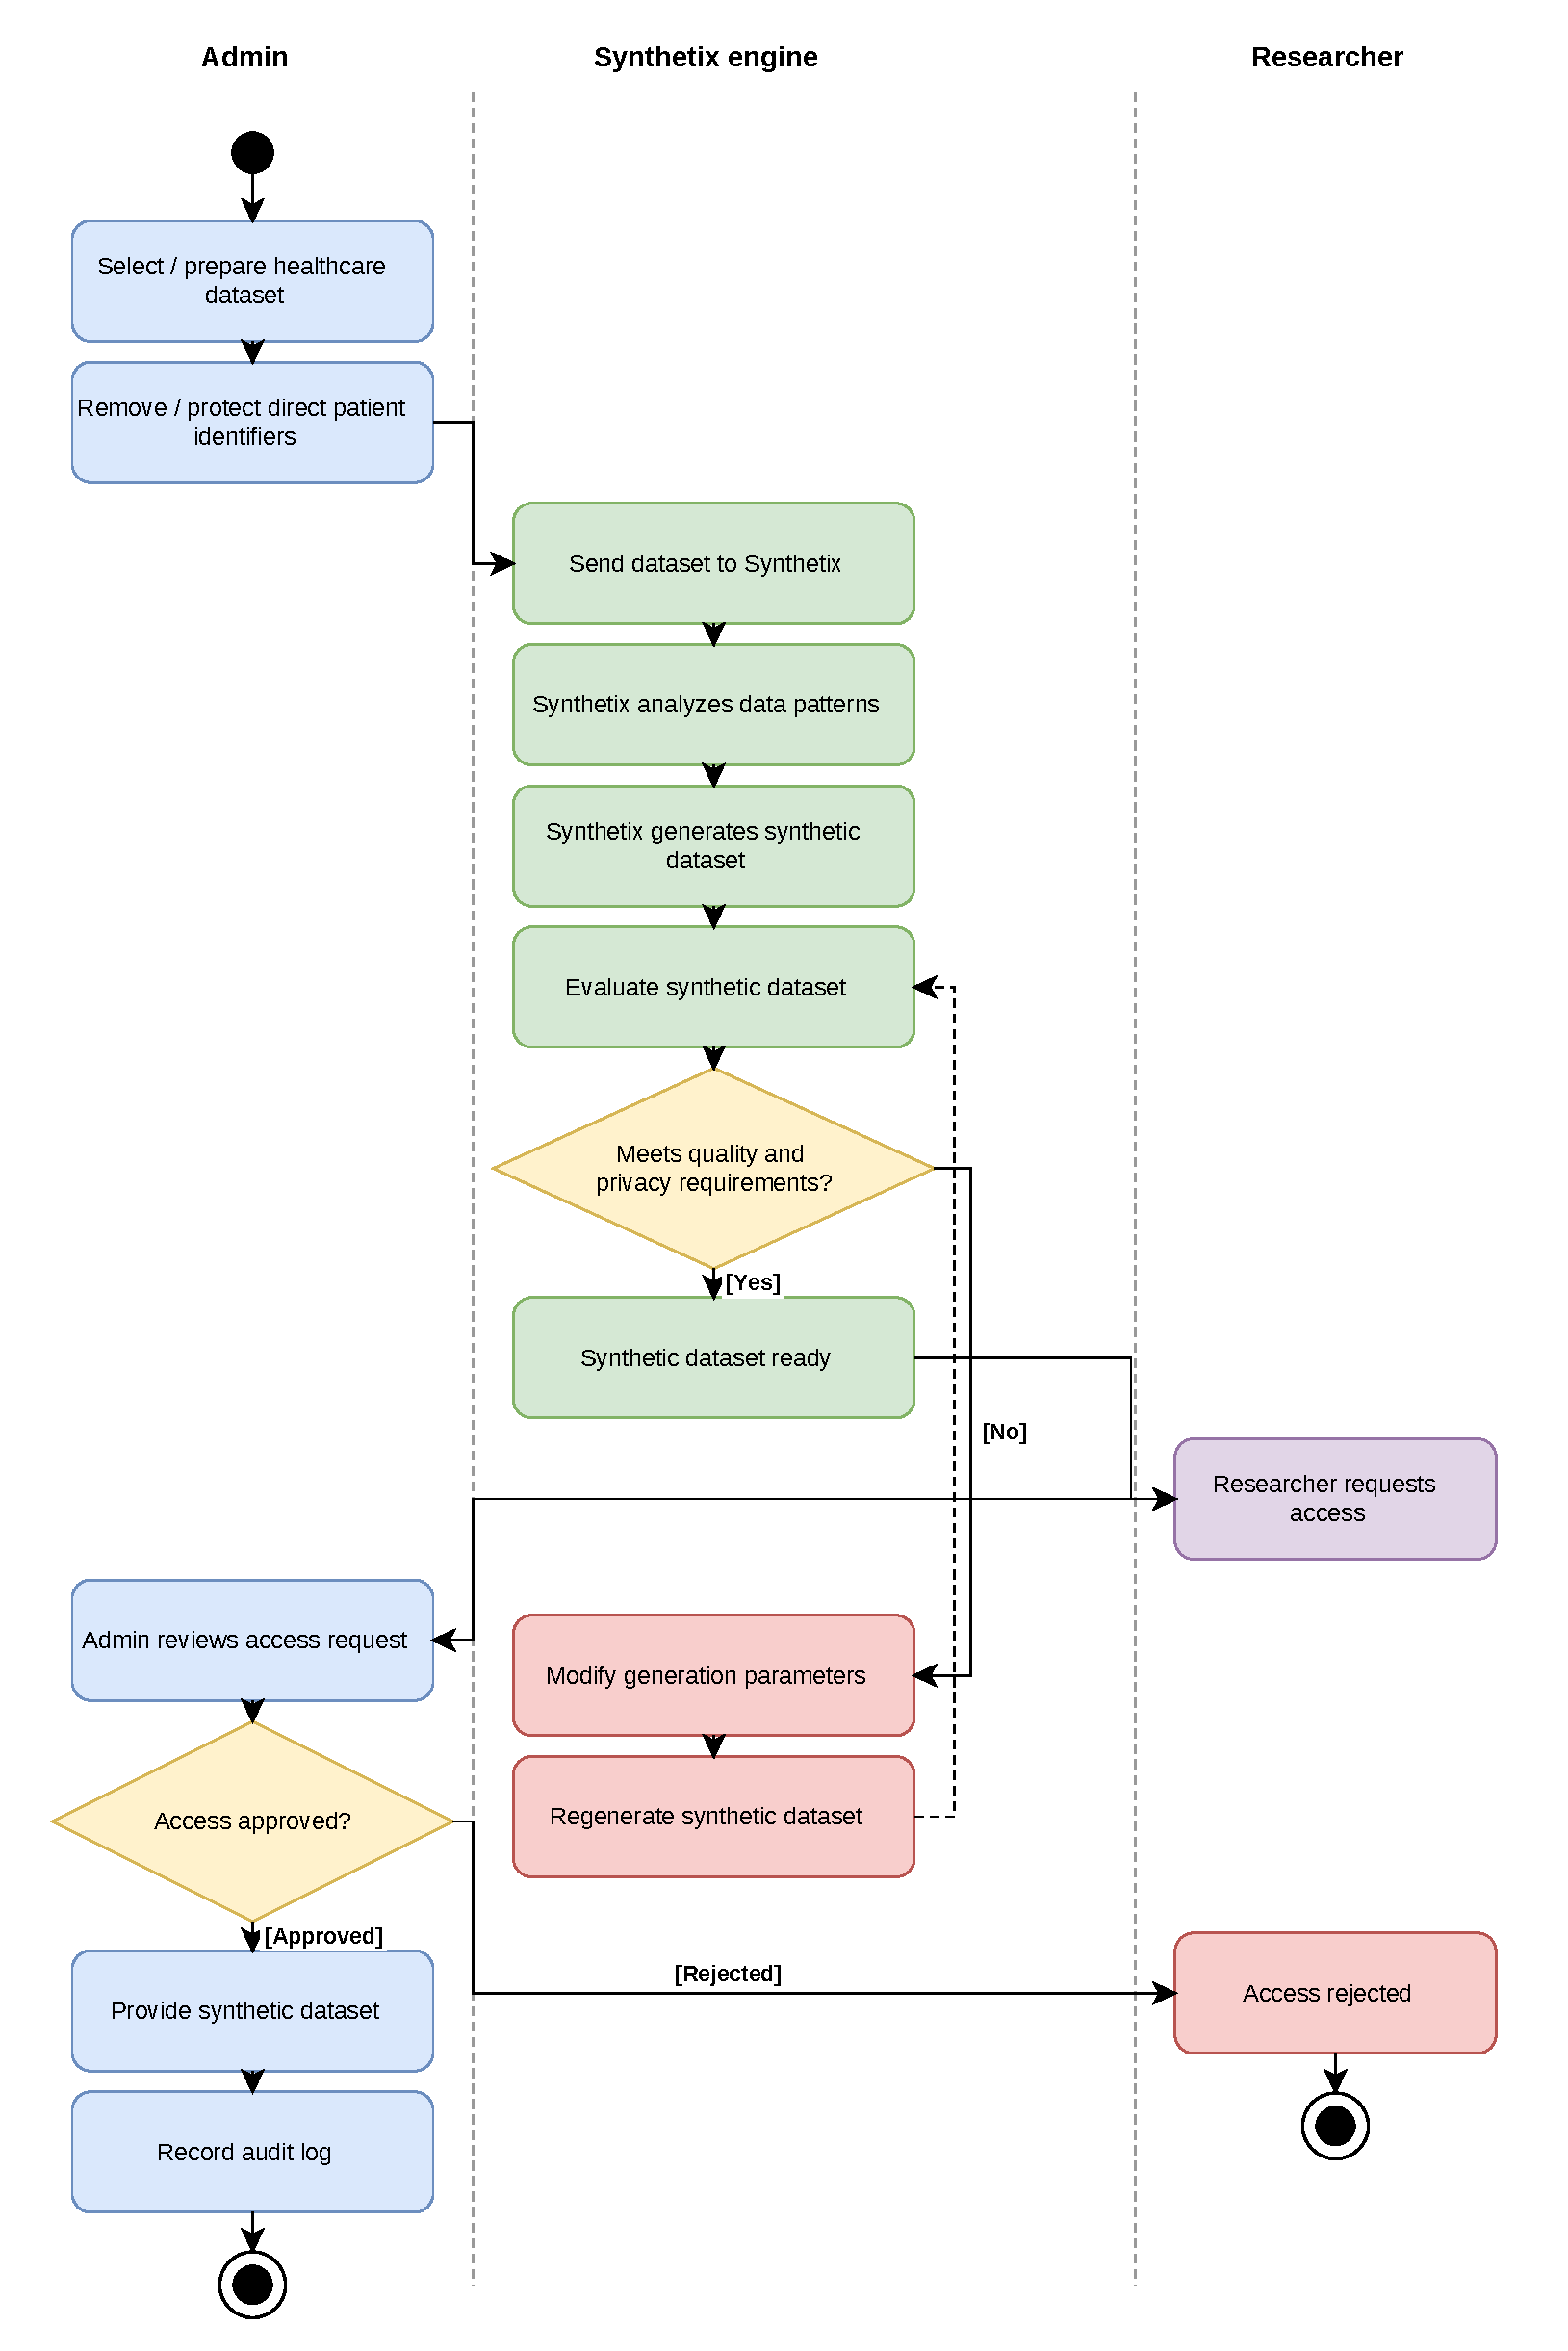
\includegraphics[width=\textwidth,height=0.72\textheight,keepaspectratio]{figures/swimlane2.pdf}
  \caption{Swimlane diagram 2: Synthetix workflow}
  \label{fig:swimlane2}
\end{figure}
\clearpage

% ----- Data flow diagrams -----
\begin{landscape}
\section{Data Flow Diagram: Level 0 (Context Diagram)}

\begin{figure}[H]
  \centering
  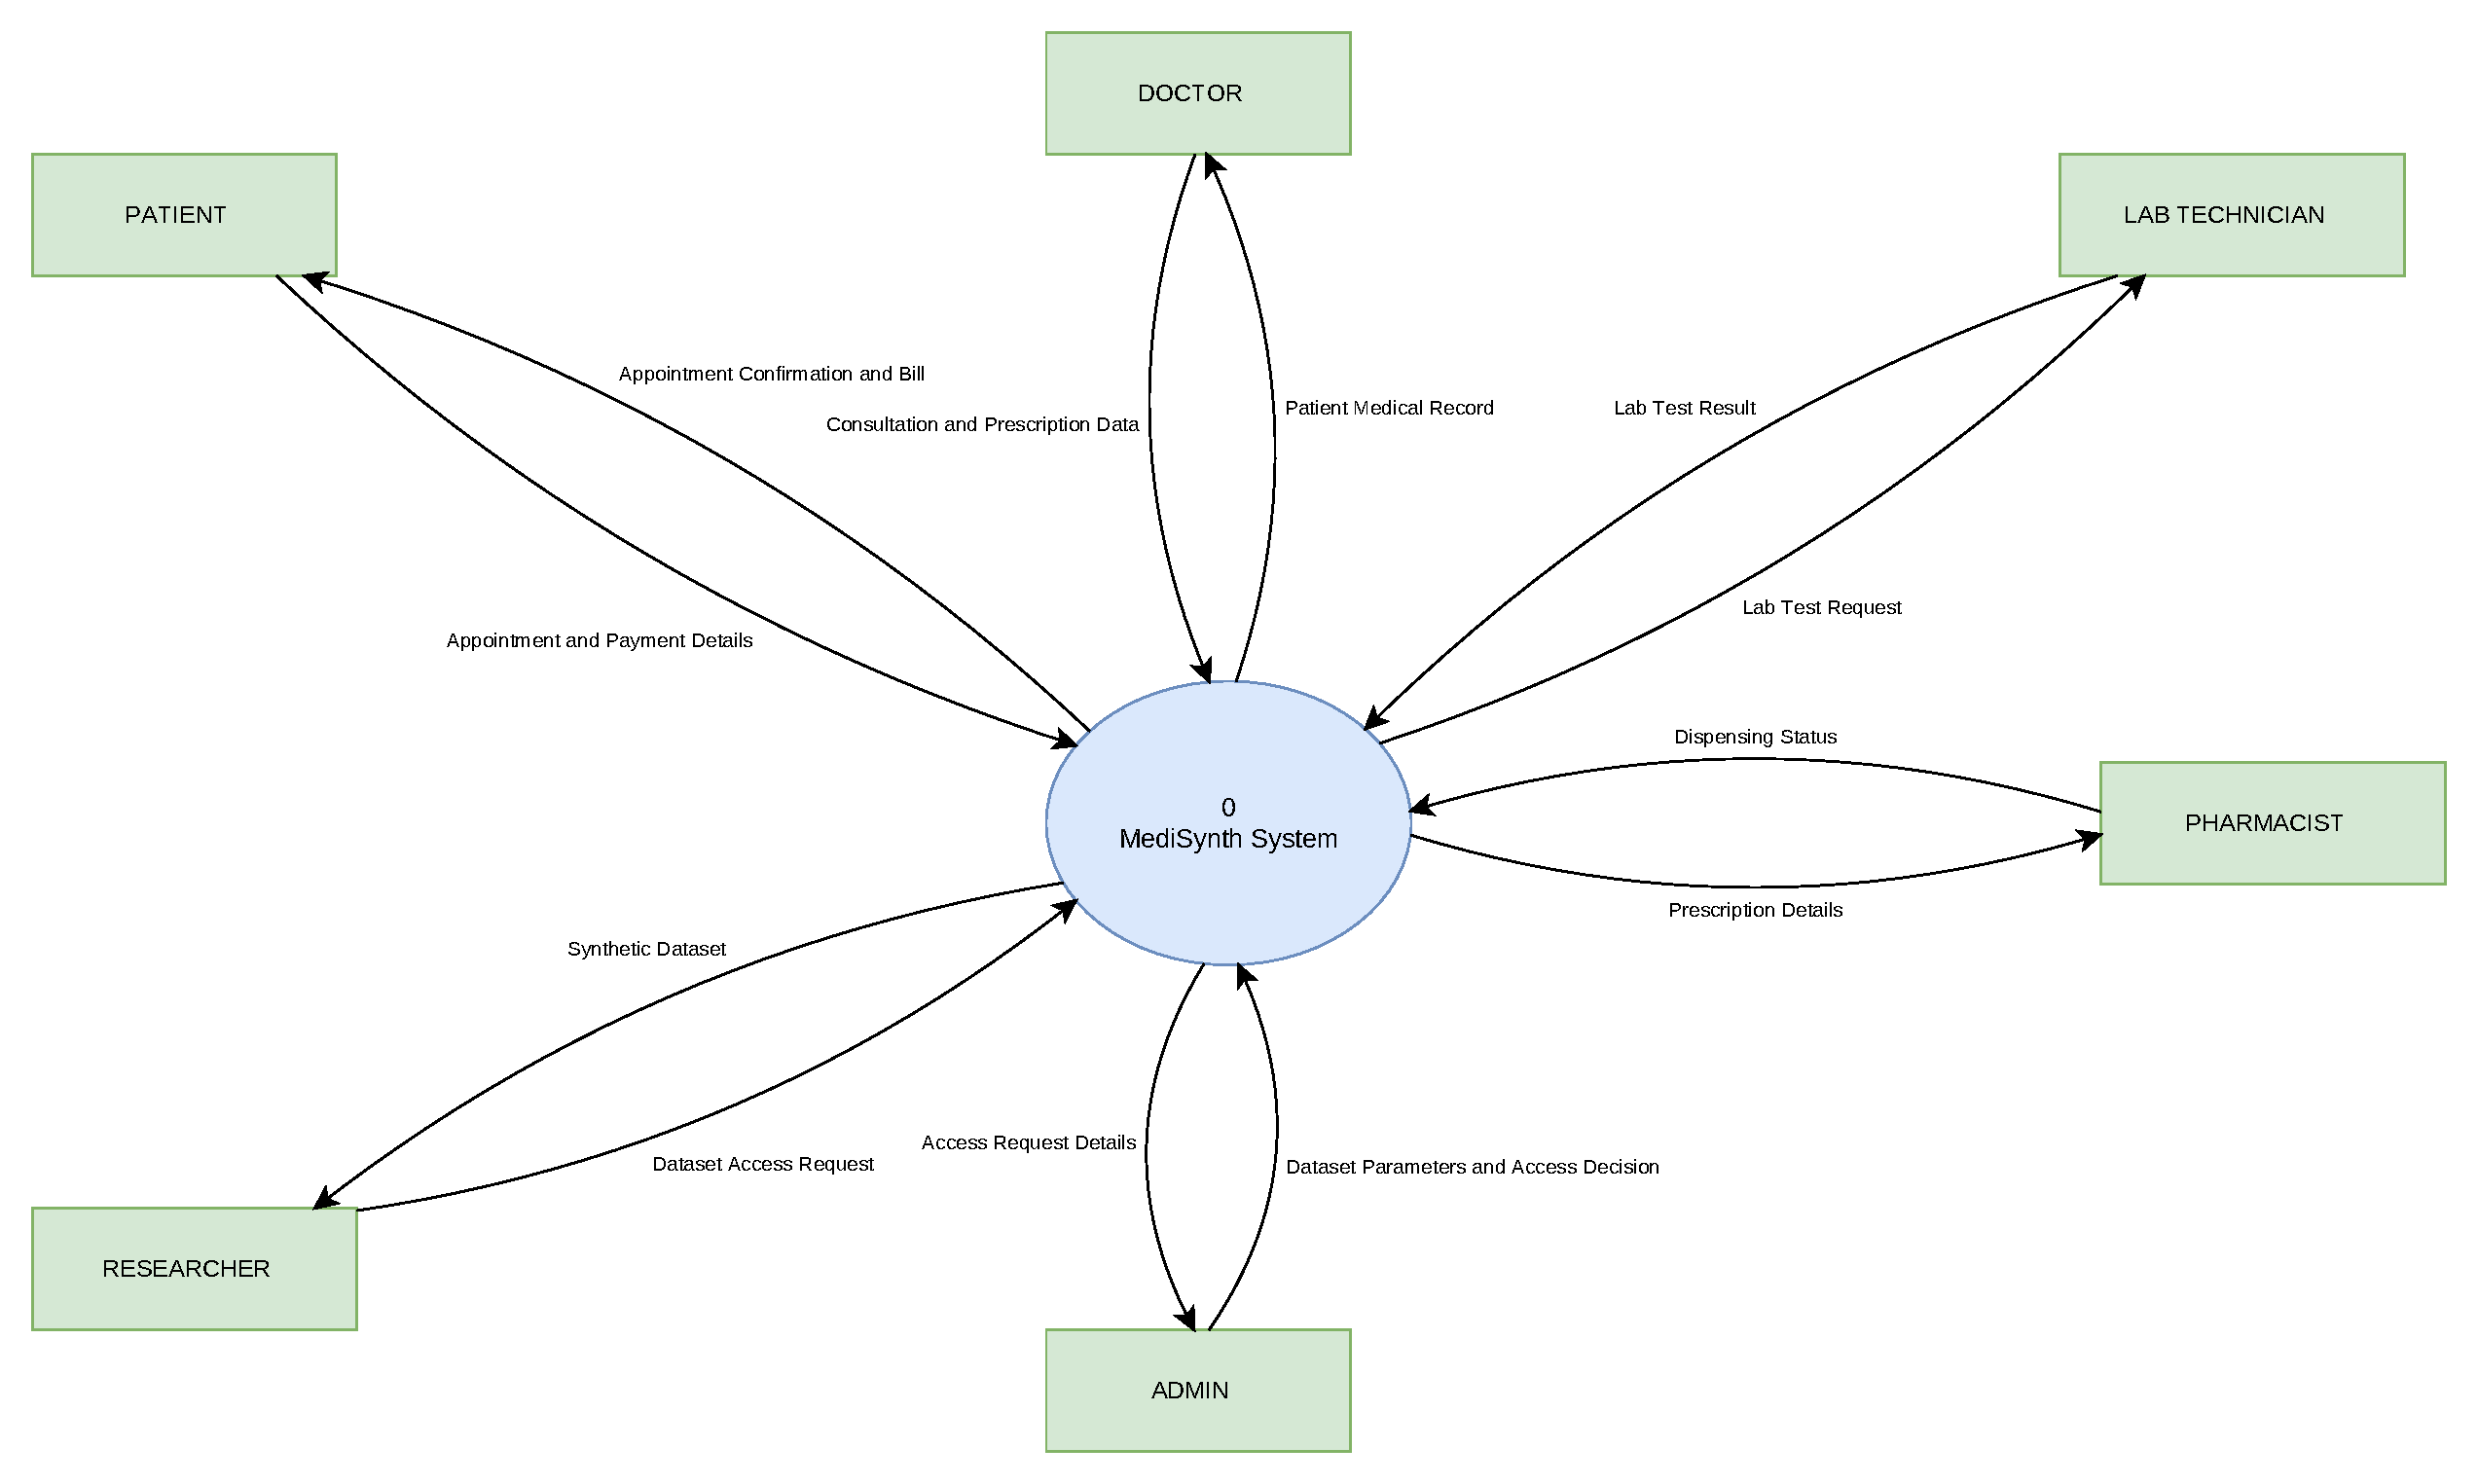
\includegraphics[width=\linewidth,height=0.82\textheight,keepaspectratio]{figures/dfd0.pdf}
  \caption{Data flow diagram: level 0 (context diagram)}
  \label{fig:dfd0}
\end{figure}
\end{landscape}

\begin{landscape}
\section{Data Flow Diagram: Level 1}
\begin{figure}[H]
  \centering
  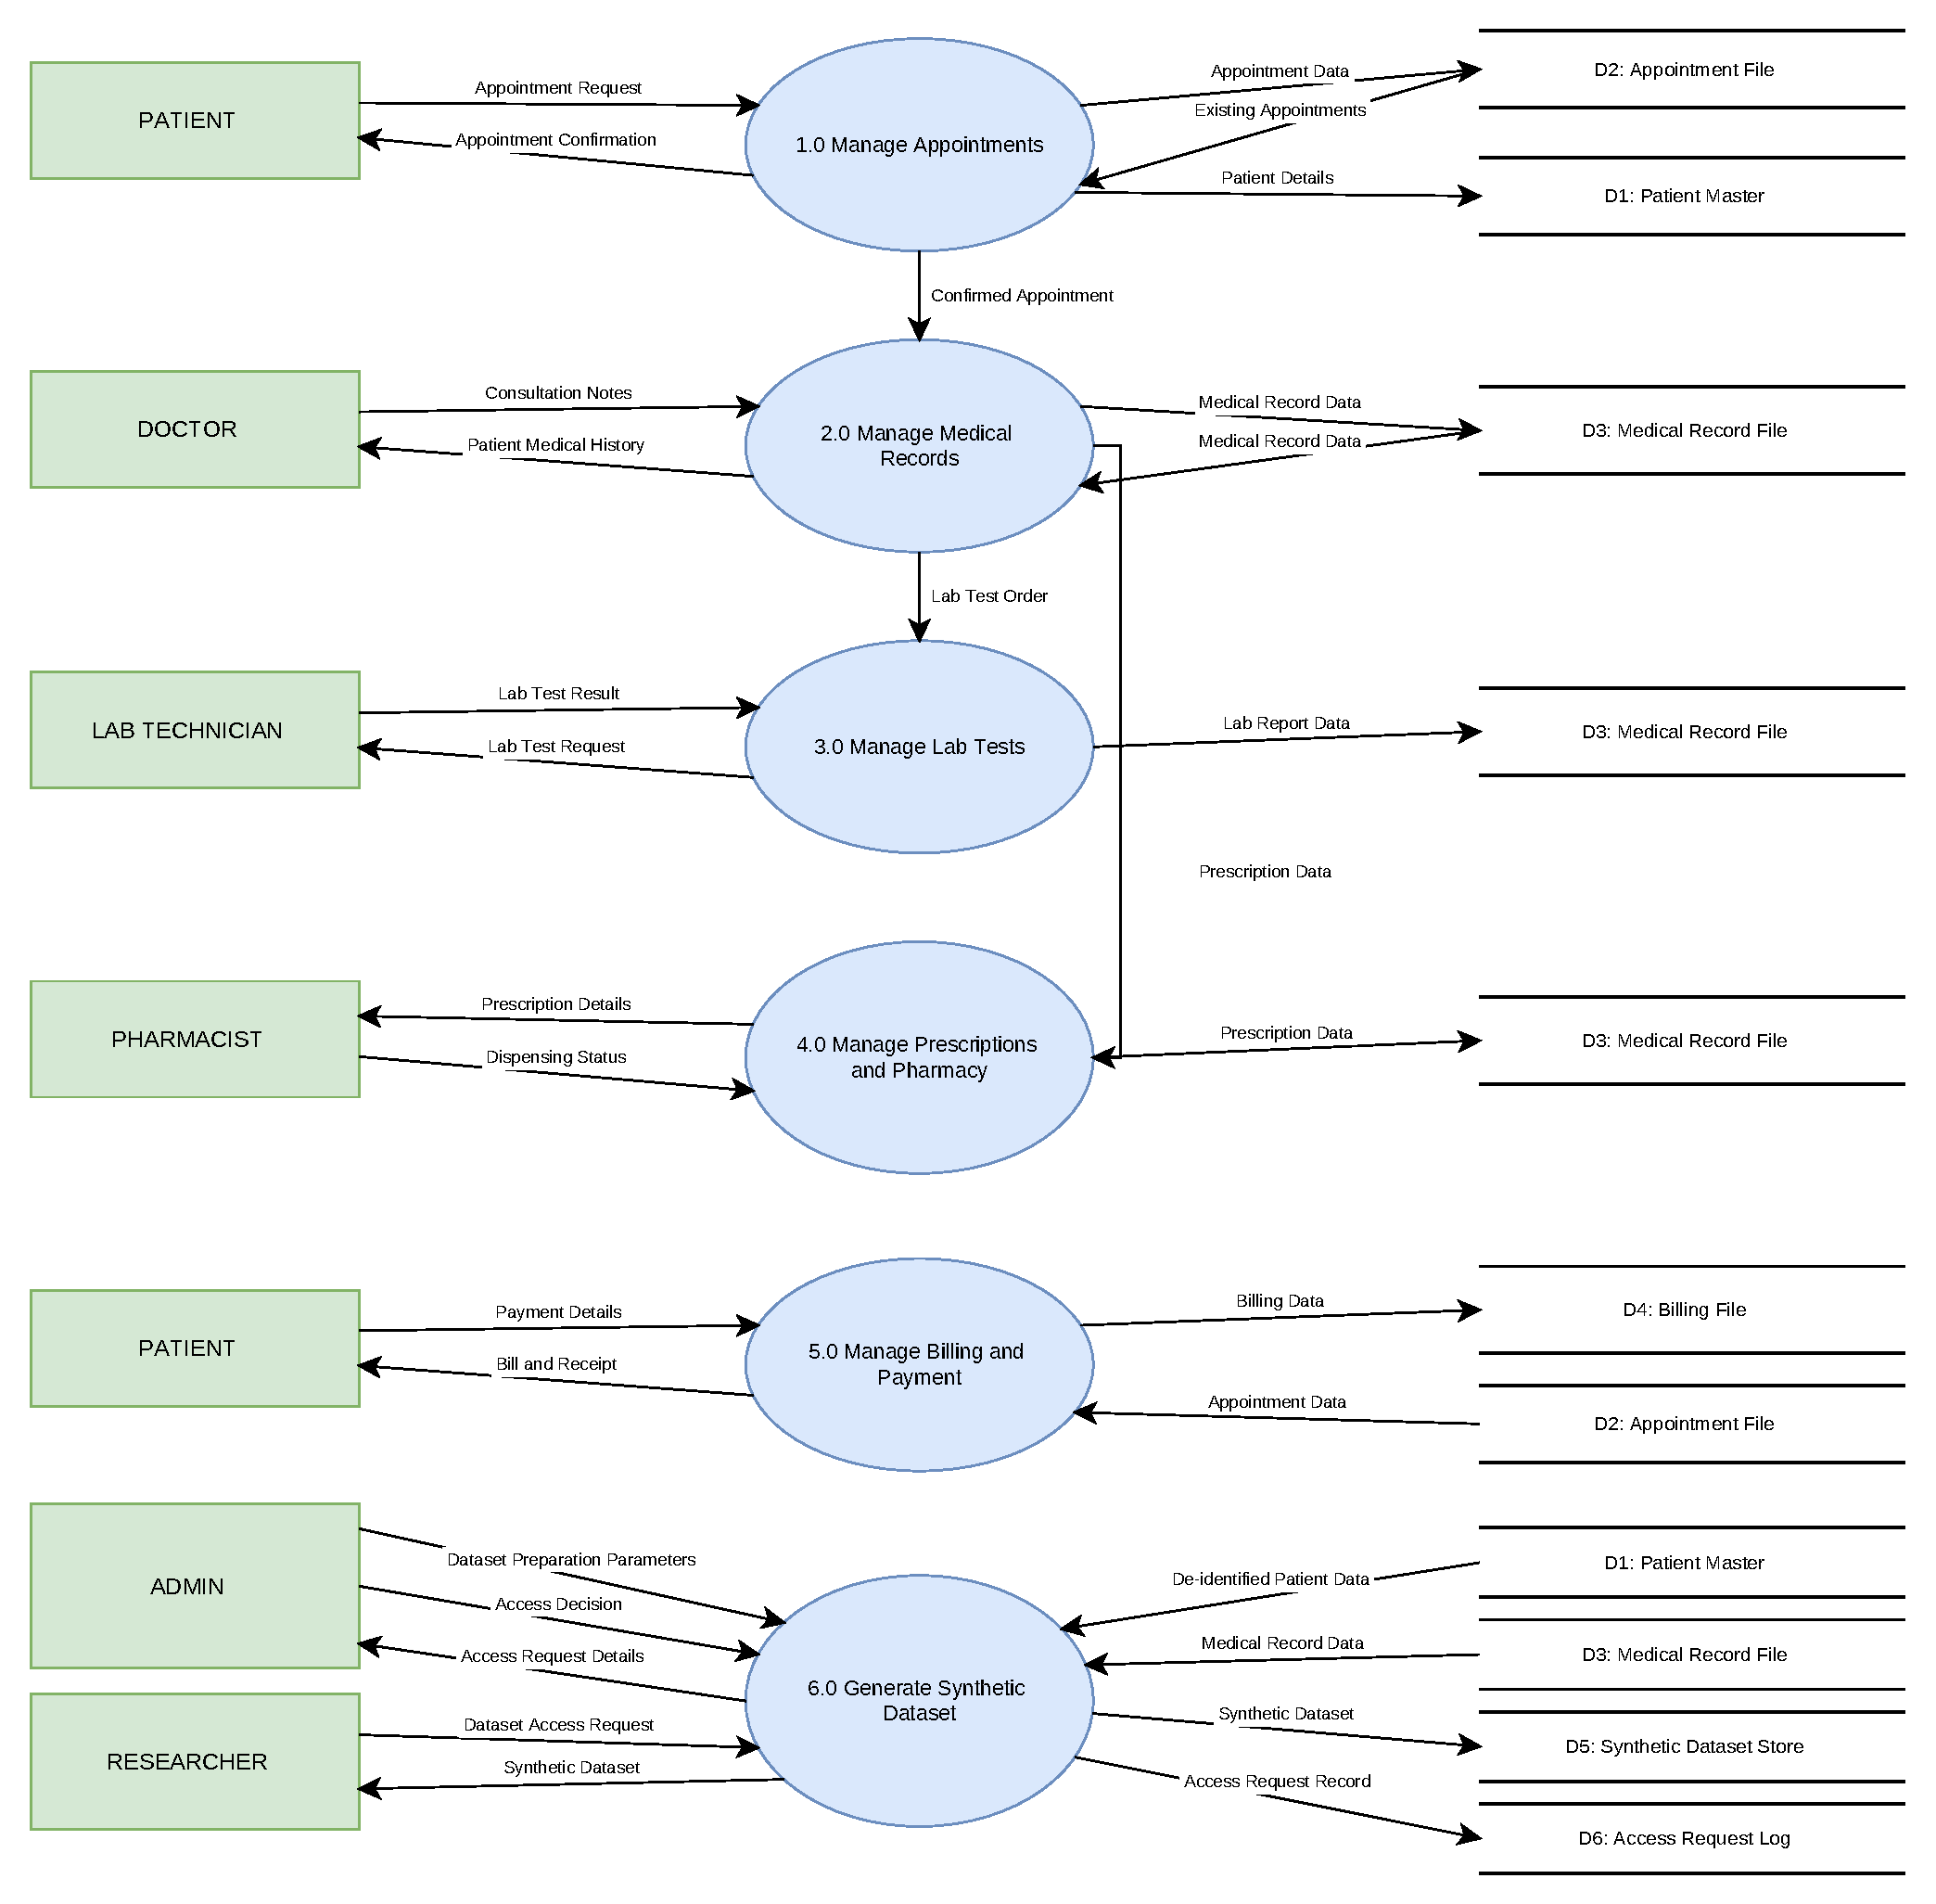
\includegraphics[width=\linewidth,height=0.82\textheight,keepaspectratio]{figures/dfd1.pdf}
  \caption{Data flow diagram: level 1}
  \label{fig:dfd1}
\end{figure}
\end{landscape}

% ----- Sequence diagrams -----
\section{Sequence Diagram 1: Book Appointment}

\begin{figure}[H]
  \centering
  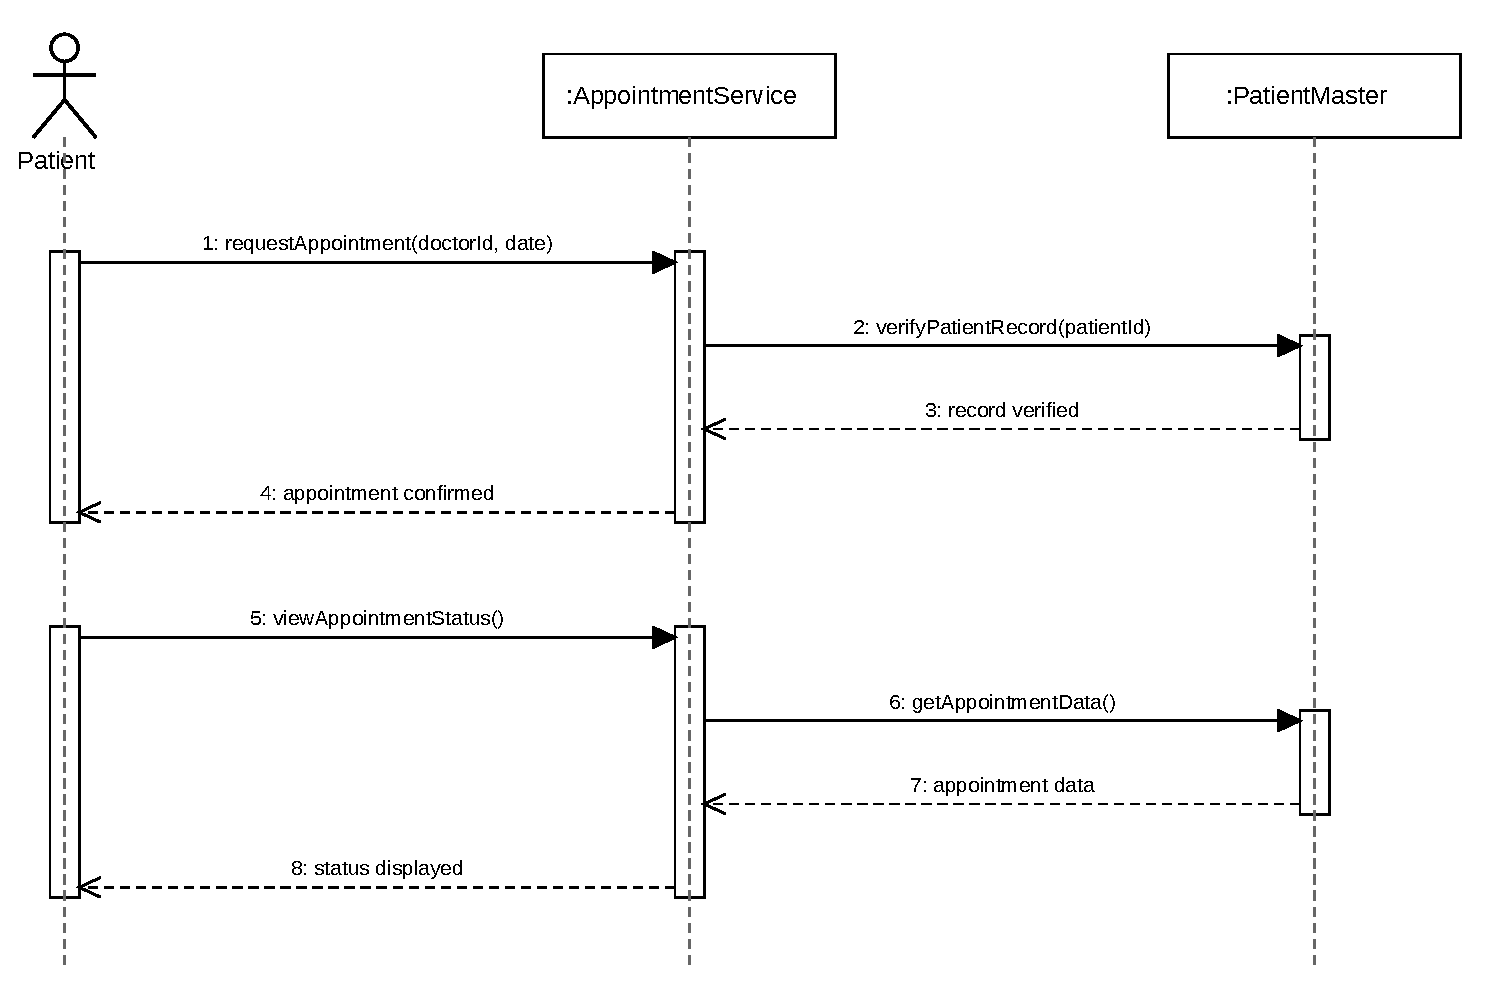
\includegraphics[width=\textwidth,height=0.72\textheight,keepaspectratio]{figures/seq1.pdf}
  \caption{Sequence diagram 1: book appointment}
  \label{fig:seq1}
\end{figure}
\clearpage

\begin{landscape}
\section{Sequence Diagram 2: Generate Synthetic Dataset}

\begin{figure}[H]
  \centering
  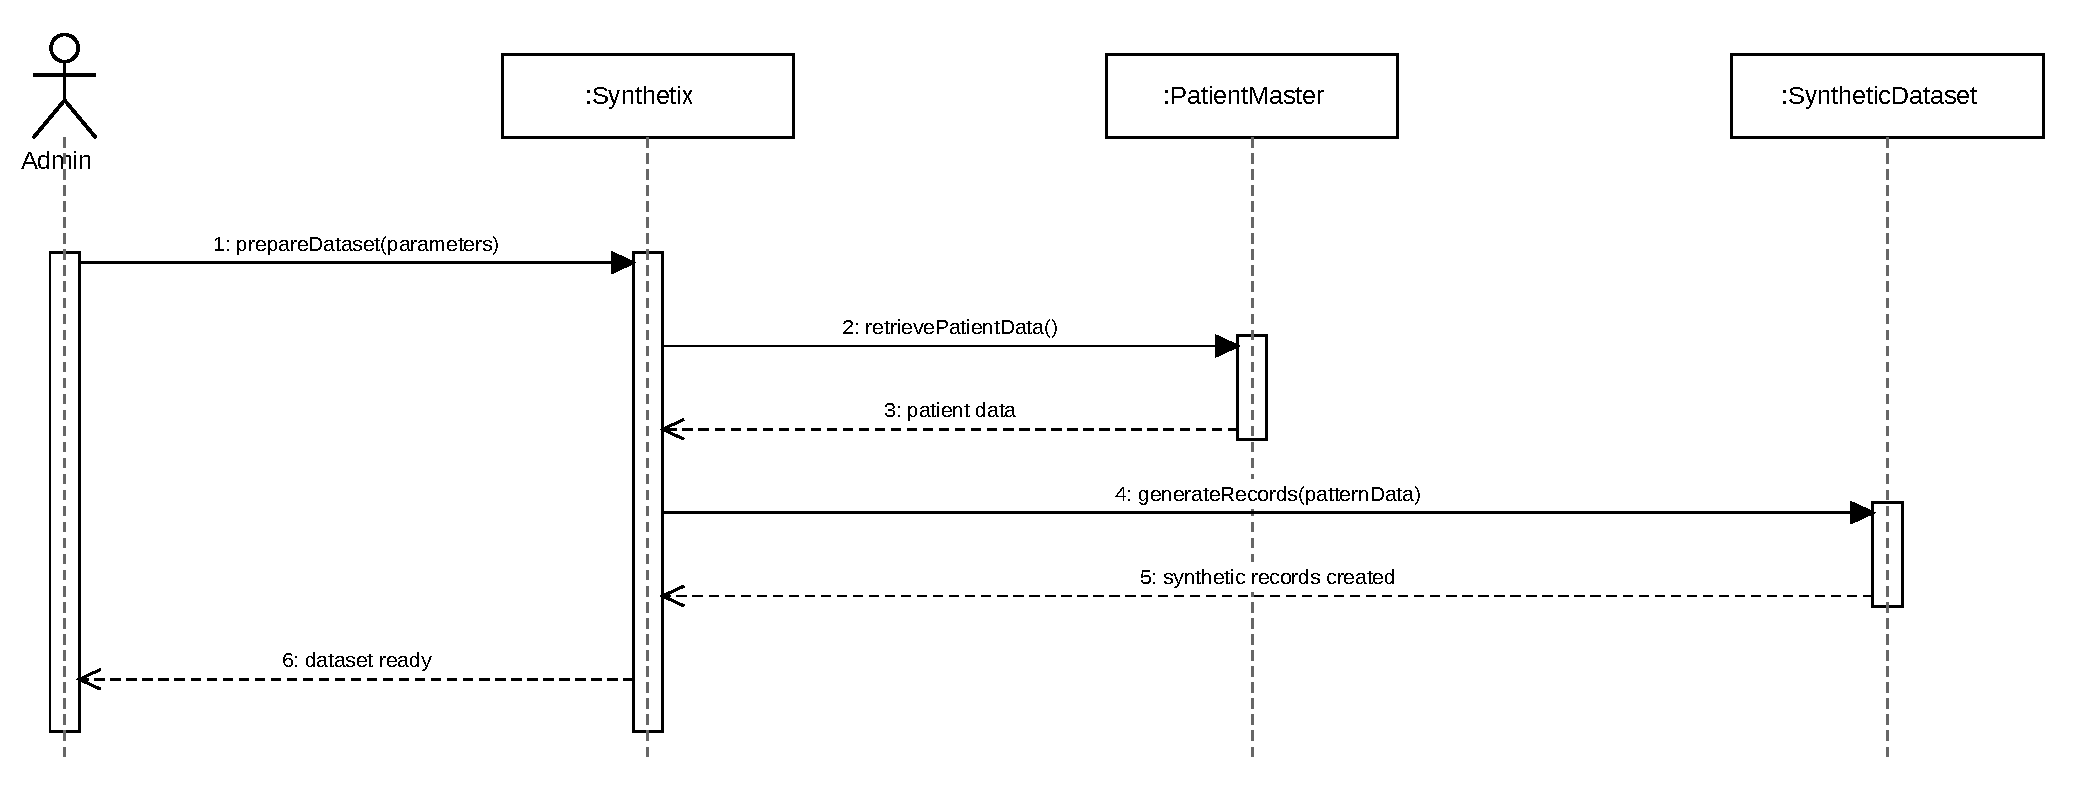
\includegraphics[width=\linewidth,height=0.82\textheight,keepaspectratio]{figures/seq2.pdf}
  \caption{Sequence diagram 2: generate synthetic dataset}
  \label{fig:seq2}
\end{figure}
\end{landscape}

% ----- Collaboration diagrams -----
\begin{landscape}
\section{Collaboration Diagram 1: Book Appointment}

\begin{figure}[H]
  \centering
  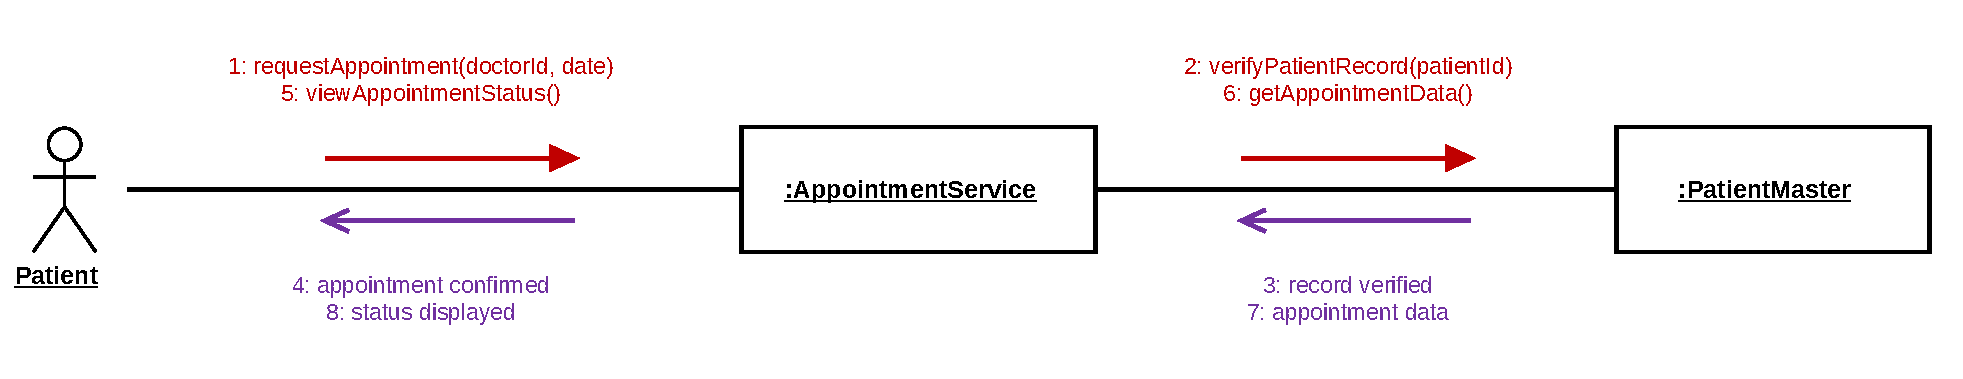
\includegraphics[width=\linewidth,height=0.82\textheight,keepaspectratio]{figures/collab1.pdf}
  \caption{Collaboration diagram 1: book appointment}
  \label{fig:collab1}
\end{figure}
\end{landscape}

\begin{landscape}
\section{Collaboration Diagram 2: Generate Synthetic Dataset}

\begin{figure}[H]
  \centering
  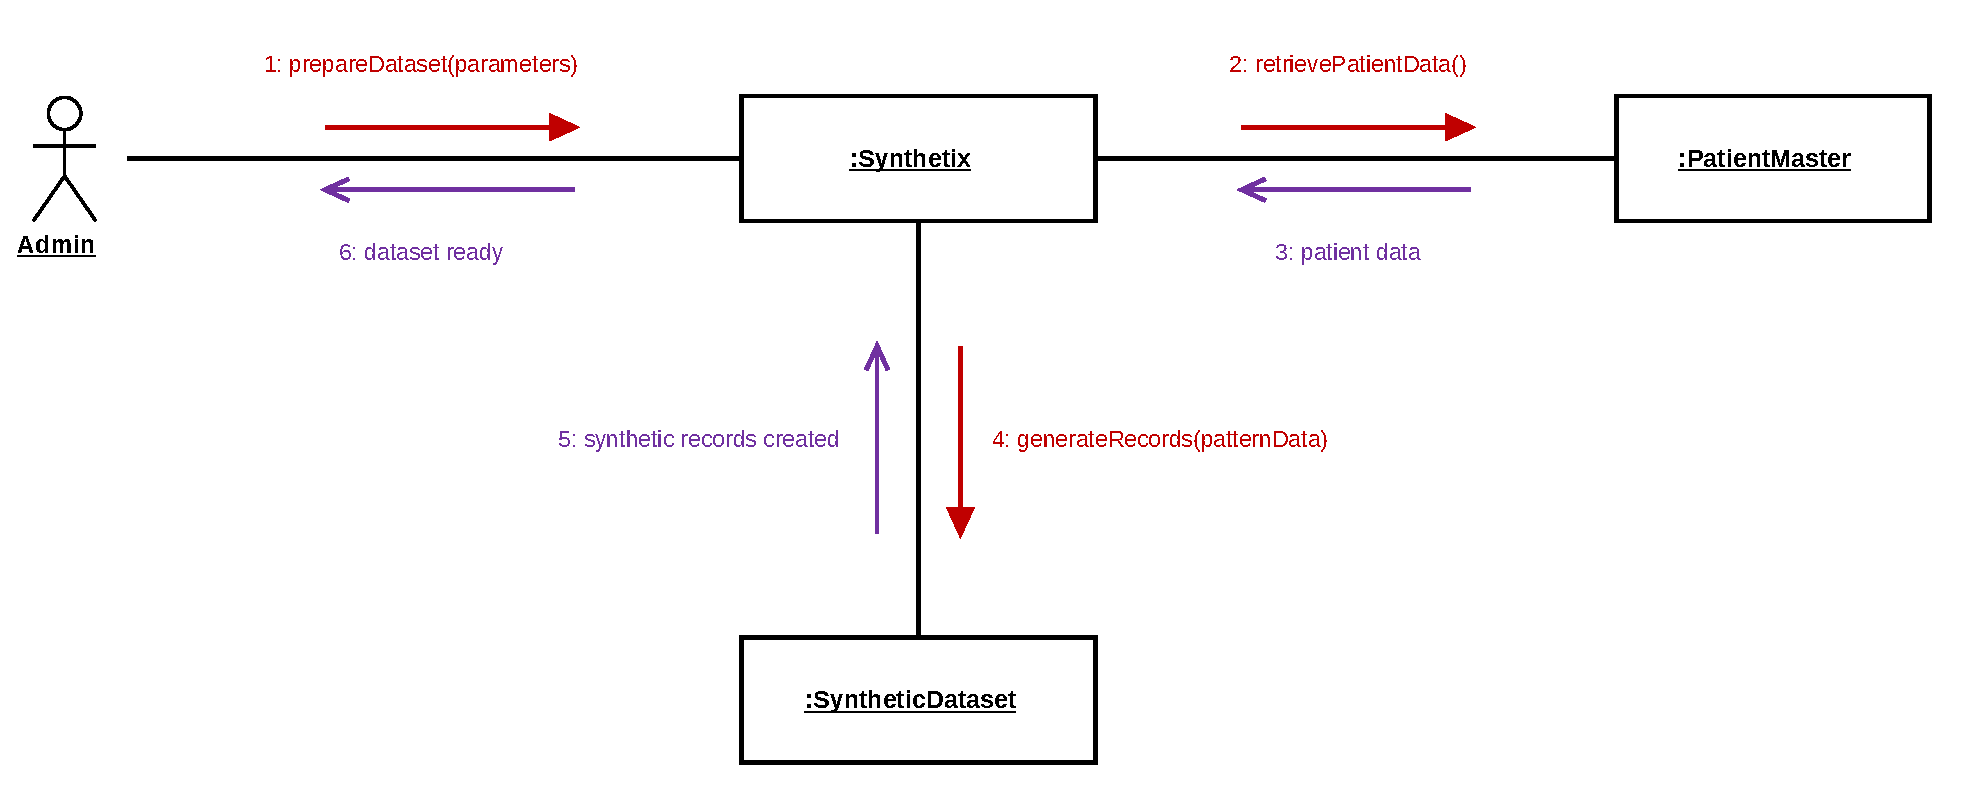
\includegraphics[width=\linewidth,height=0.82\textheight,keepaspectratio]{figures/collab2.pdf}
  \caption{Collaboration diagram 2: generate synthetic dataset}
  \label{fig:collab2}
\end{figure}
\end{landscape}

% ----- State diagrams -----
\begin{landscape}
\section{State Diagram 1: Appointment}

\begin{figure}[H]
  \centering
  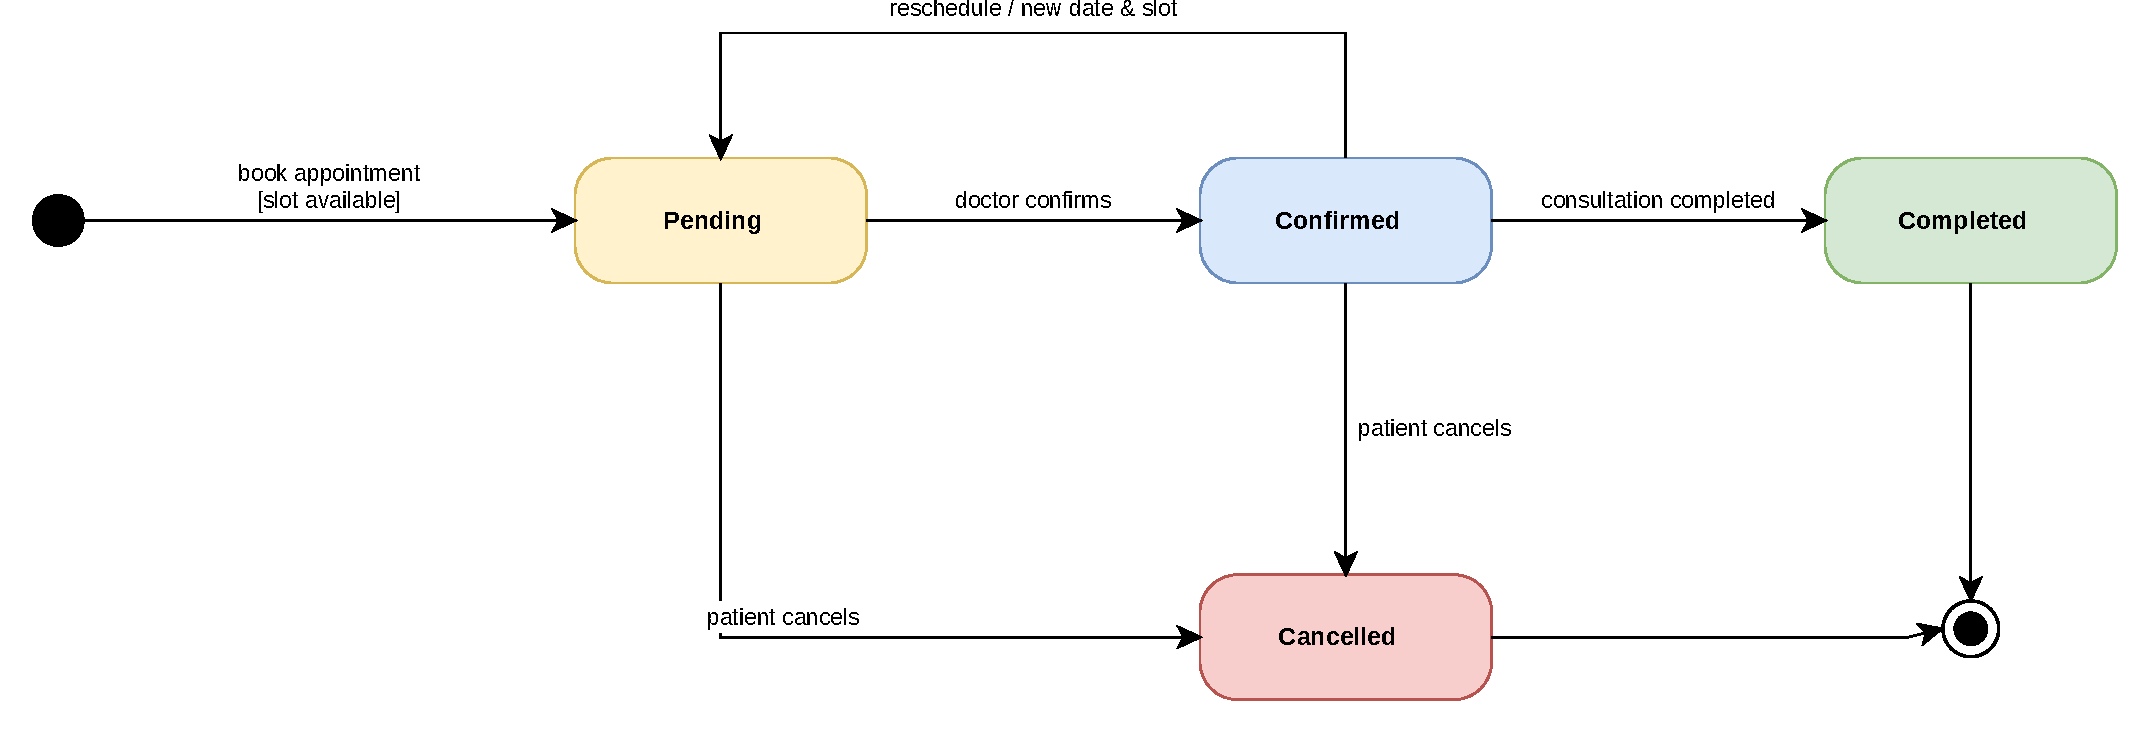
\includegraphics[width=\linewidth,height=0.82\textheight,keepaspectratio]{figures/state1.pdf}
  \caption{State diagram 1: appointment}
  \label{fig:state1}
\end{figure}
\end{landscape}

\begin{landscape}
\section{State Diagram 2: Bill and Payment}

\begin{figure}[H]
  \centering
  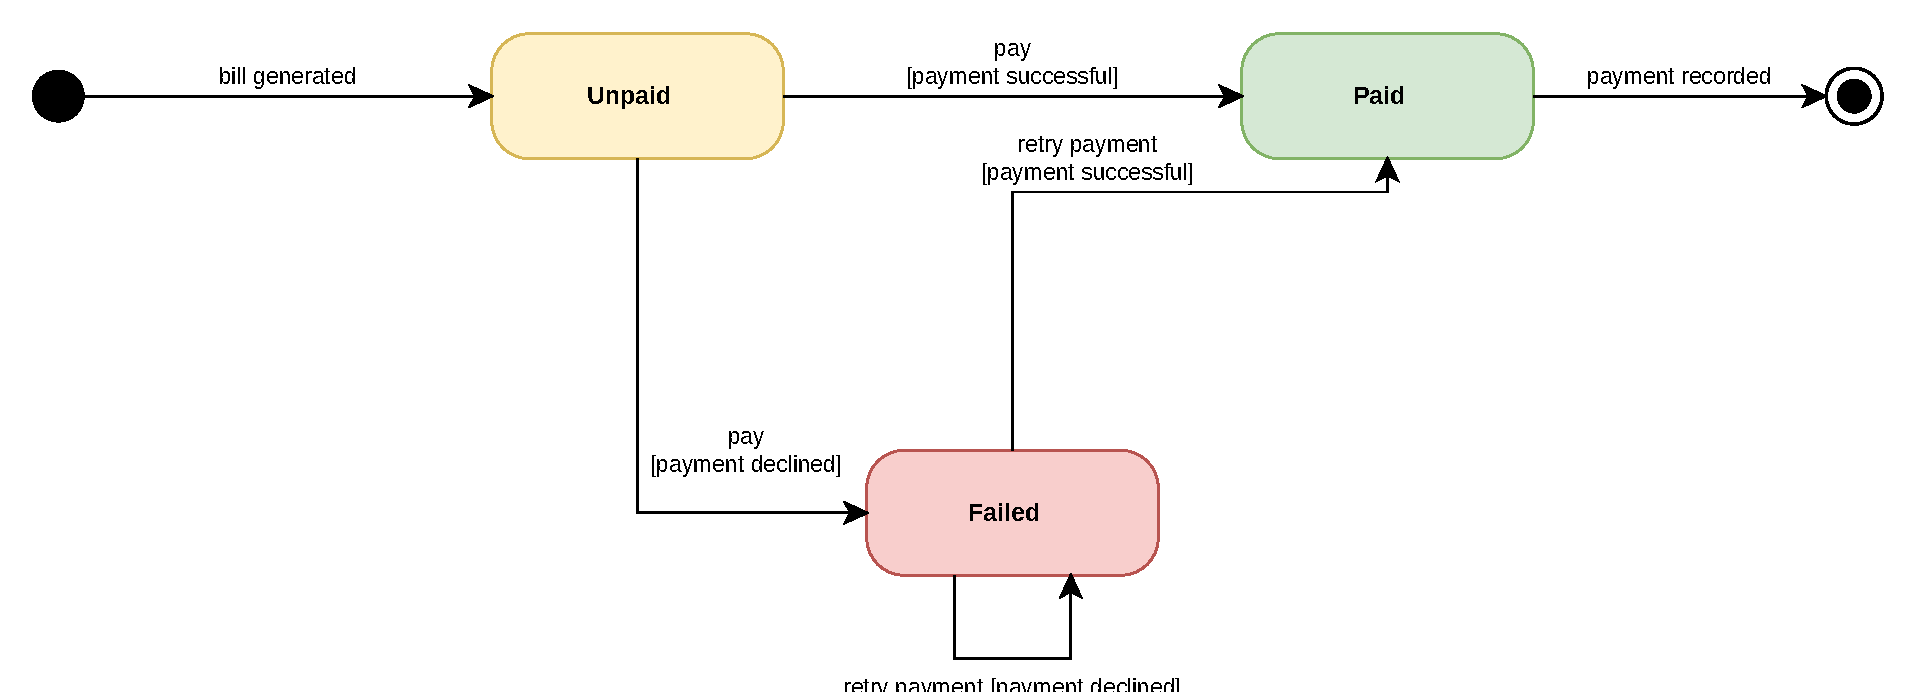
\includegraphics[width=\linewidth,height=0.82\textheight,keepaspectratio]{figures/state2.pdf}
  \caption{State diagram 2: bill and payment}
  \label{fig:state2}
\end{figure}
\end{landscape}

\begin{landscape}
\section{State Diagram 3: Synthetic Dataset}

\begin{figure}[H]
  \centering
  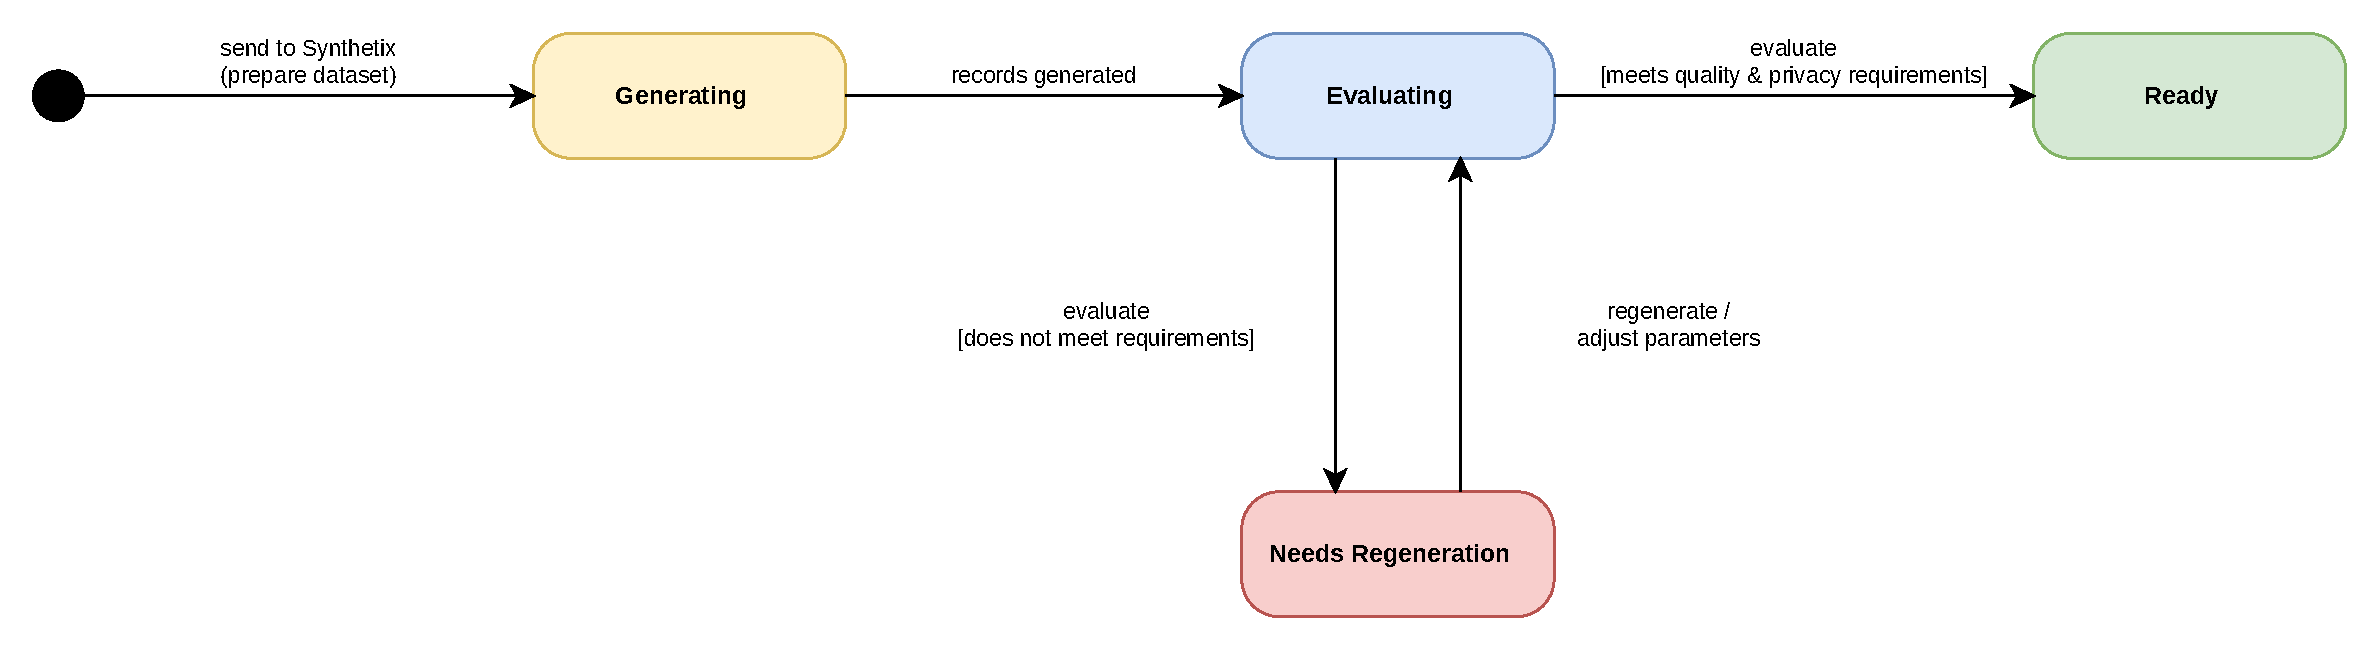
\includegraphics[width=\linewidth,height=0.82\textheight,keepaspectratio]{figures/state3.pdf}
  \caption{State diagram 3: synthetic dataset}
  \label{fig:state3}
\end{figure}
\end{landscape}

% ----- Component diagram -----
\begin{landscape}
\section{Component Diagram}
\begin{figure}[H]
  \centering
  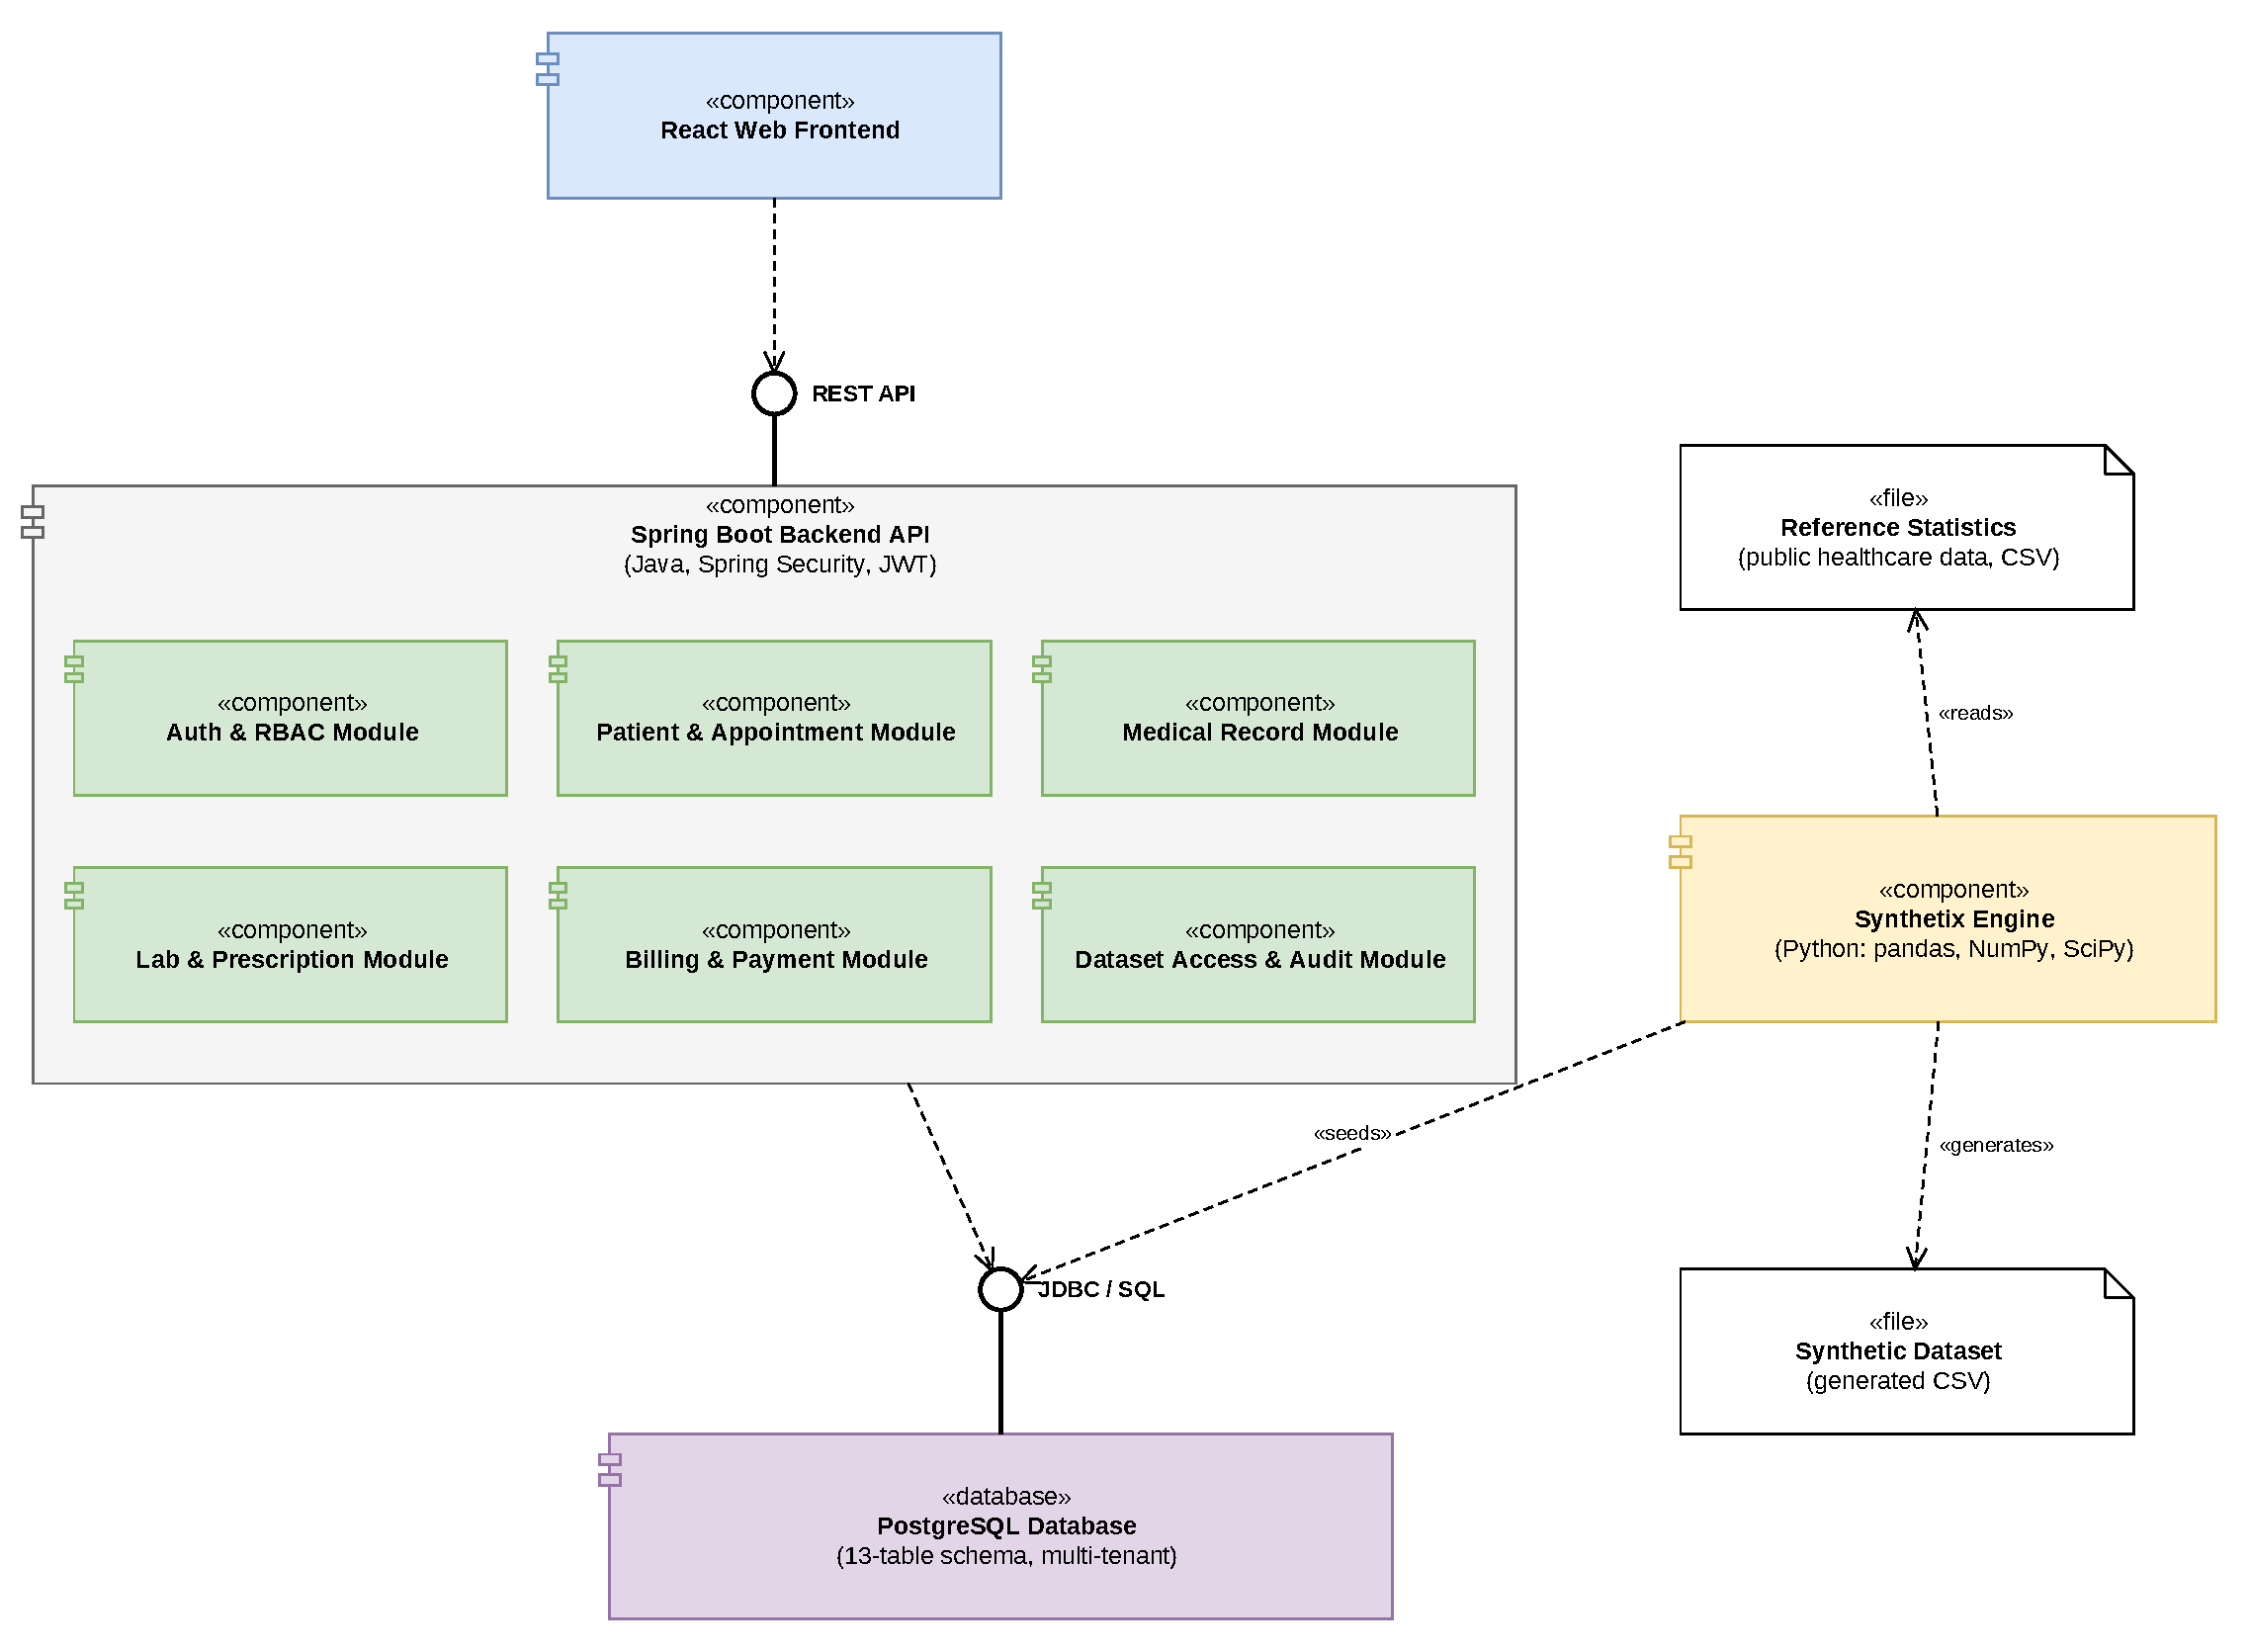
\includegraphics[width=\linewidth,height=0.66\textheight,keepaspectratio]{figures/component.pdf}
  \caption{Component diagram for MediSynth}
  \label{fig:component}
  \par\small Note: this diagram shows the mid-semester design with a Python Synthetix engine; in the final build the engine is a Java package inside the Spring Boot backend (see the deployment diagram).
\end{figure}
\end{landscape}


% ----- Deployment diagram (as built) -----
\begin{landscape}
\section{Deployment Diagram (as built)}

The mid-semester design showed a separate Synthetix server. In the final build
Synthetix runs inside the application server, so the deployment is simpler.

\begin{figure}[H]
  \centering
  \begin{tikzpicture}[
      node distance=1.6cm and 2.4cm,
      dev/.style={draw,thick,rounded corners=2pt,fill=blue!8,minimum width=4.2cm,minimum height=2cm,align=center,font=\small},
      art/.style={font=\scriptsize\itshape},
      link/.style={-{Stealth},thick,font=\scriptsize,align=center}]
    \node[dev] (client) {\textbf{User device}\\ \scriptsize{}«device»\\ \scriptsize{}web browser};
    \node[dev,right=of client,fill=green!10] (web) {\textbf{Web server}\\ \scriptsize{}«node»\\ \scriptsize{}React build (Vite)};
    \node[dev,right=of web,fill=orange!12] (app) {\textbf{Application server}\\ \scriptsize{}«node», Java 21\\ \scriptsize{}Spring Boot API\\ \scriptsize{}+ Synthetix engine};
    \node[dev,right=of app,fill=violet!10] (db) {\textbf{Database server}\\ \scriptsize{}«node»\\ \scriptsize{}PostgreSQL 16\\ \scriptsize{}Flyway V1--V3};
    \draw[link] (client) -- node[above]{«HTTPS»} (web);
    \draw[link] (web.south) to[bend right=25] node[below]{static files} (client.south);
    \draw[link] (client.north) to[bend left=30] node[above]{«HTTPS REST / JSON»\\ Bearer token} (app.north);
    \draw[link] (app) -- node[above]{«JDBC / SQL»} (db);
  \end{tikzpicture}
  \caption{Deployment diagram for MediSynth (as built)}
  \label{fig:deployment}
\end{figure}
\end{landscape}

% ===== CHAPTER 4: RESULTS AND EVALUATION =====

\chapter{Results and Evaluation}
\label{ch:results}

\section{Testing Methodology}

\begin{itemize}
  \item \textbf{Unit testing:} the Synthetix engine has no framework
    dependencies, so its generator and evaluator are tested directly
    (\texttt{SyntheticEngineTest}); JWT handling and the password-strength
    validator have their own unit tests.
  \item \textbf{Integration testing:} 11 Spring Boot test classes run the real
    application against a separate PostgreSQL database
    (\texttt{medisynth\_test}), covering registration and login, admin
    provisioning, registration approval, access control, appointments, lab
    tests, rate limiting, research requests, synthetic datasets and data
    persistence across restarts. The suite contains 108 test methods in 14
    classes.
  \item \textbf{Functional (black-box) testing:} three end-to-end test cases
    were designed from the use cases and executed through the web interface
    (Section~\ref{sec:tc}).
  \item \textbf{Statistical evaluation of Synthetix:} generated datasets of
    several sizes and seeds were scored by the evaluator
    (Section~\ref{sec:synres}).
\end{itemize}

\section{Functional Test Cases}
\label{sec:tc}

All three cases were designed by Tanu Bansal and executed by Aryan Sharma on
17 November 2026 using the project's standard test-case template. Each step
lists the action, the expected system response, the outcome and a comment.

\begin{table}[H]
\centering
\small
\begin{tabular}{p{1.0cm}p{4.2cm}p{5.6cm}p{1.6cm}}
\toprule
\textbf{No.} & \textbf{Test case} & \textbf{What it verifies} & \textbf{Result} \\
\midrule
1.1 & First admin bootstrap and access control & Admin can be created only with the bootstrap secret; a second admin is refused; a patient cannot open admin pages & Pass \\
2.1 & Doctor registration, approval and login & A doctor cannot log in until approved; the server decides the role; duplicate email refused & Pass \\
3.1 & Appointment booking and slot conflict handling & A free slot can be booked; the same slot returns 409; the doctor can confirm & Pass \\
\bottomrule
\end{tabular}
\caption{Functional test cases (outcomes as recorded in the test-case sheets)}
\label{tab:tc}
\end{table}

\section{Synthetix Evaluation Results}
\label{sec:synres}

Each dataset size was generated with three different seeds and scored by the
evaluator using the built-in source profile. Table~\ref{tab:engine} gives the
mean over the three seeds. Validity was 1.000 in every run.

\begin{table}[H]
\centering
\small
\begin{tabular}{rccccccc}
\toprule
\textbf{Records} & \textbf{Overall} & \textbf{Marginal} & \textbf{Relat.} & \textbf{Privacy} & \textbf{In $k\!\ge\!5$} & \textbf{Unique} & \textbf{Passed} \\
\midrule
500 & 0.747 & 0.950 & 0.958 & 0.242 & 61.9\% & 7.53\% & 0/3 \\
2{,}000 & 0.951 & 0.969 & 1.000 & 0.872 & 93.5\% & 1.25\% & 0/3 \\
5{,}000 & 0.976 & 0.974 & 1.000 & 0.951 & 98.0\% & 0.58\% & 3/3 \\
10{,}000 & 0.983 & 0.975 & 1.000 & 0.974 & 98.7\% & 0.26\% & 3/3 \\
\bottomrule
\end{tabular}
\caption{Synthetix evaluator scores by dataset size (mean of 3 seeds)}
\label{tab:engine}
\end{table}

\paragraph{Fidelity and relationships.} Marginal fidelity is high at every
size (0.95--0.98). At 5,000 records the age band, gender, blood group and
diagnosis distributions are within 0.022 total variation distance of the
reference, and the means of all numeric columns are within a few per cent of
their reference values (for example systolic pressure 121.0 against 120.0
mmHg and total cholesterol 182.4 against 182.0 mg/dL). All eight clinical
relationship checks pass at 5,000 and 10,000 records (Table~\ref{tab:rel}).

\begin{table}[H]
\centering
\small
\begin{tabular}{p{8.2cm}cc}
\toprule
\textbf{Relationship} & \textbf{Observed} & \textbf{Needed} \\
\midrule
Older patients have higher systolic pressure (correlation) & 0.64 & 0.20 \\
Diabetic patients: higher fasting glucose (mg/dL) & +71.9 & +35 \\
Hypertensive patients: higher systolic pressure (mmHg) & +28.6 & +12 \\
Kidney disease: higher creatinine (mg/dL) & +1.79 & +0.6 \\
Hyperlipidaemia: higher cholesterol (mg/dL) & +45.4 & +25 \\
Heart, lung, kidney disease admitted more often (ratio) & 9.9 & 2.0 \\
Chronic conditions have more visits (difference) & +2.16 & +0.8 \\
COPD patients smoke more (ratio) & 2.9 & 2.0 \\
\bottomrule
\end{tabular}
\caption{Clinical relationship checks, 5,000 records, seed 1}
\label{tab:rel}
\end{table}

\paragraph{Privacy.} Privacy is what decides whether a dataset can be
released. With only 500 records, 7.5\% of records are unique on age band,
gender and diagnosis and only 62\% sit in a group of five or more, so the
dataset is rejected even though its fidelity is good. At 2,000 records the
overall score is 0.951, above the 0.90 gate, yet the dataset is still
rejected because 93.5\% (needed: 95\%) are in groups of five or more and
1.25\% (limit: 1\%) are unique. At 5,000 and 10,000 records every gate is met.
This is the intended behaviour: a high average score cannot hide a privacy
failure, and the administrator is told to regenerate with more records.

\section{Application Screenshots}
\label{sec:screens}

The screenshots below were captured from the running application on a local machine and follow one complete path through the system: a doctor registers, waits for approval, is approved by the administrator, and then works with a patient's appointment.

\begin{figure}[H]
  \centering
  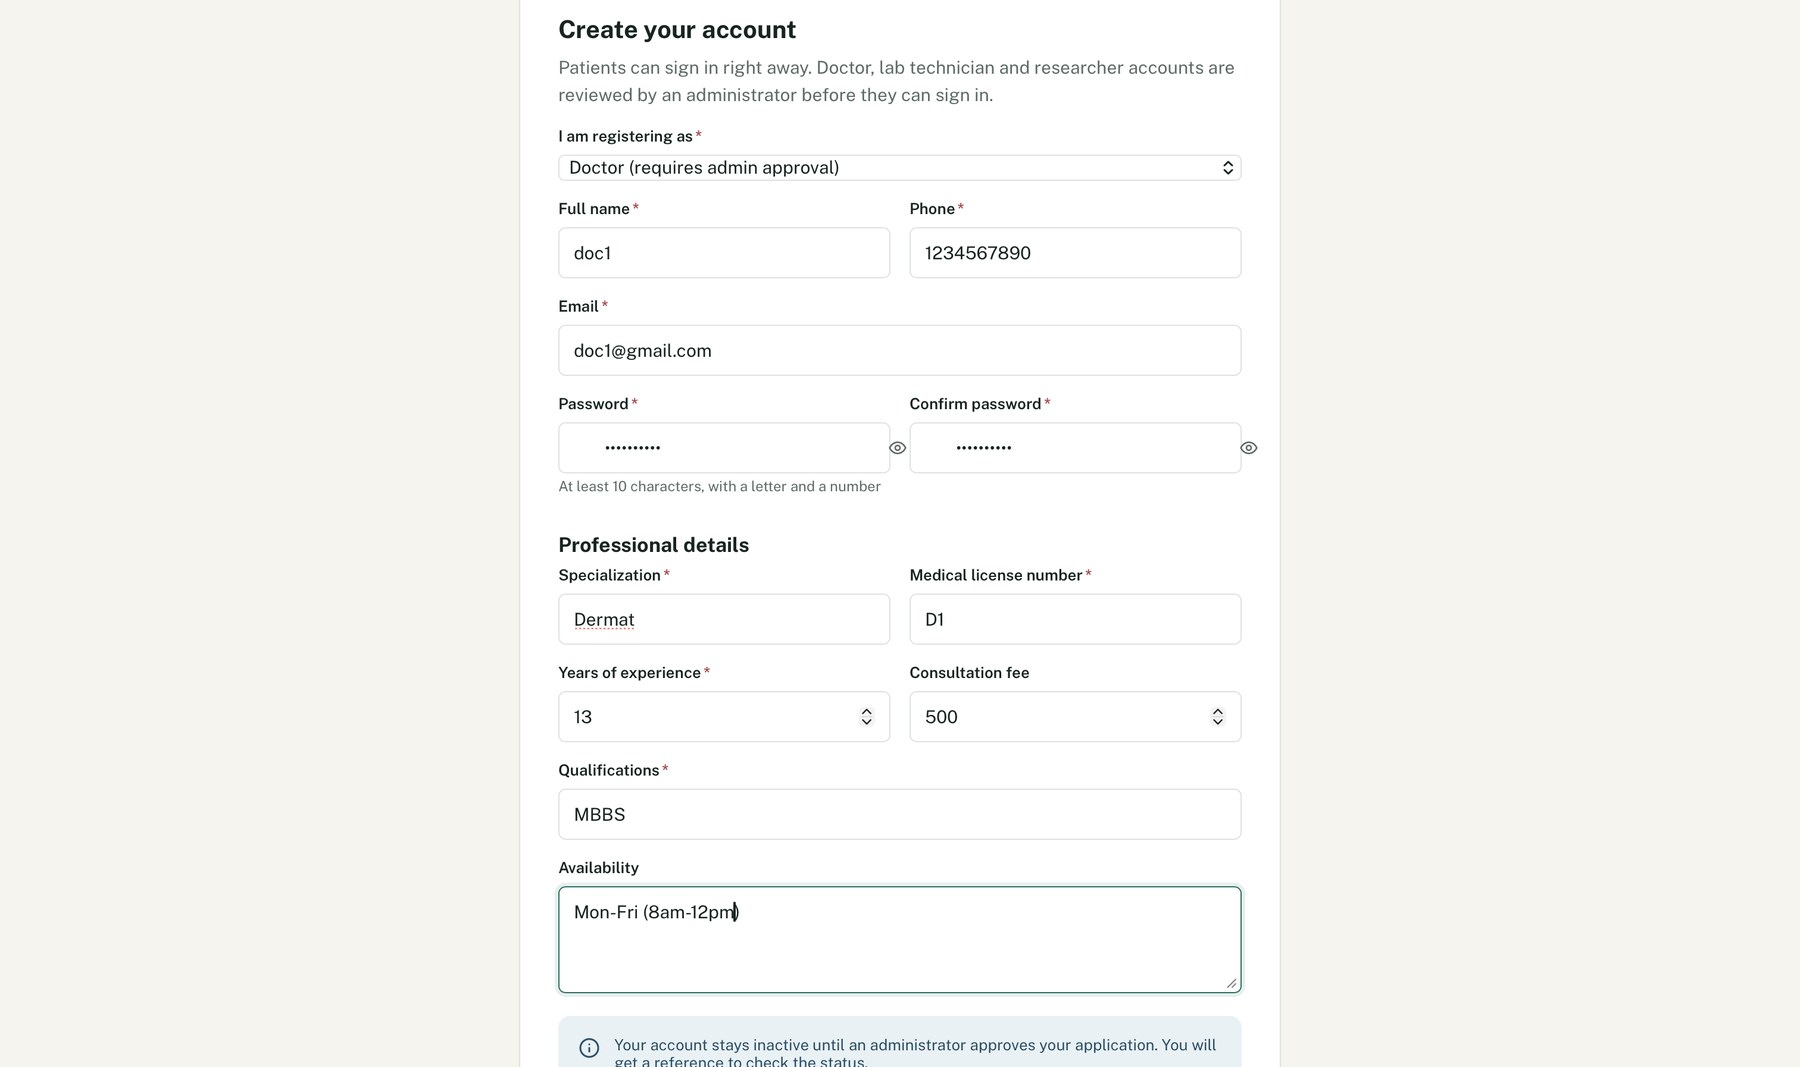
\includegraphics[width=0.95\textwidth,height=0.40\textheight,keepaspectratio]{screenshots/register.jpg}
  \caption{Registration form for a doctor, with professional details (account needs admin approval)}
  \label{fig:shot-register}
\end{figure}

\begin{figure}[H]
  \centering
  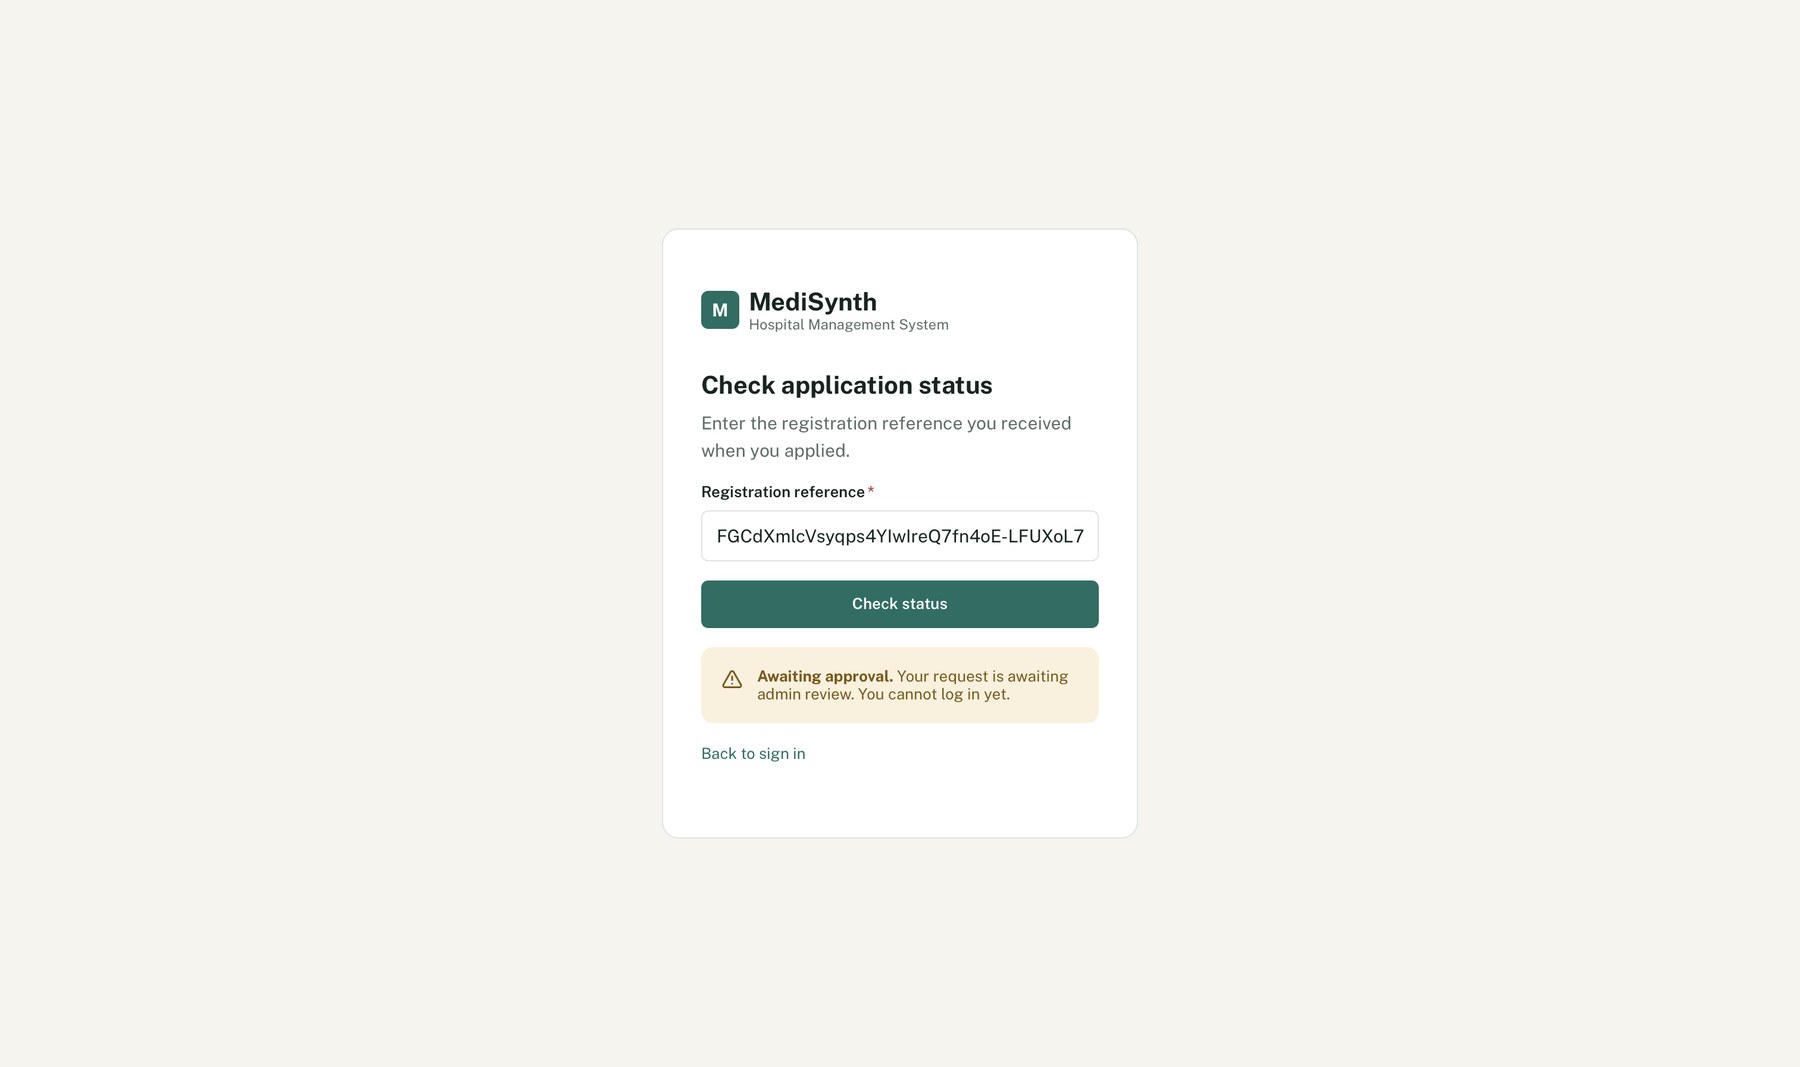
\includegraphics[width=0.95\textwidth,height=0.40\textheight,keepaspectratio]{screenshots/status.jpg}
  \caption{Application status page: the doctor sees ``Awaiting approval and cannot log in yet}
  \label{fig:shot-status}
\end{figure}

\begin{figure}[H]
  \centering
  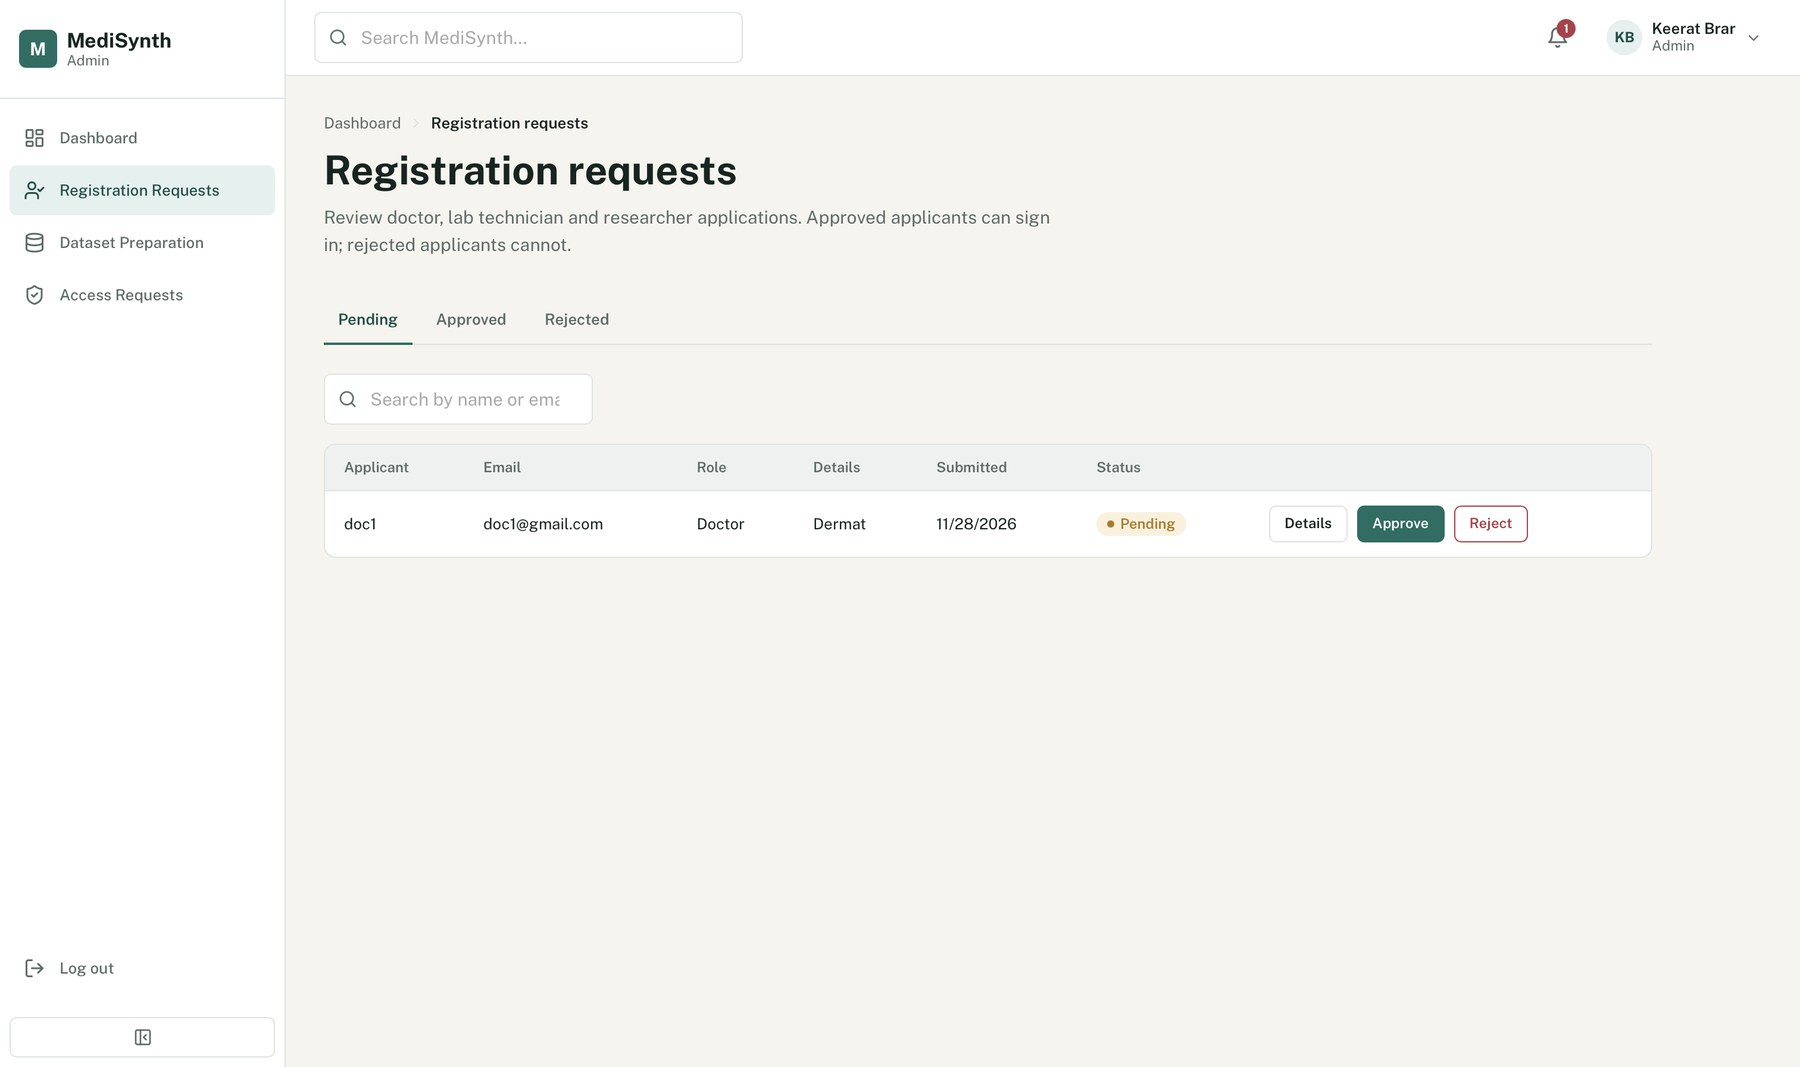
\includegraphics[width=0.95\textwidth,height=0.40\textheight,keepaspectratio]{screenshots/admin_requests.jpg}
  \caption{Administrator: registration requests list with Details, Approve and Reject actions}
  \label{fig:shot-requests}
\end{figure}

\begin{figure}[H]
  \centering
  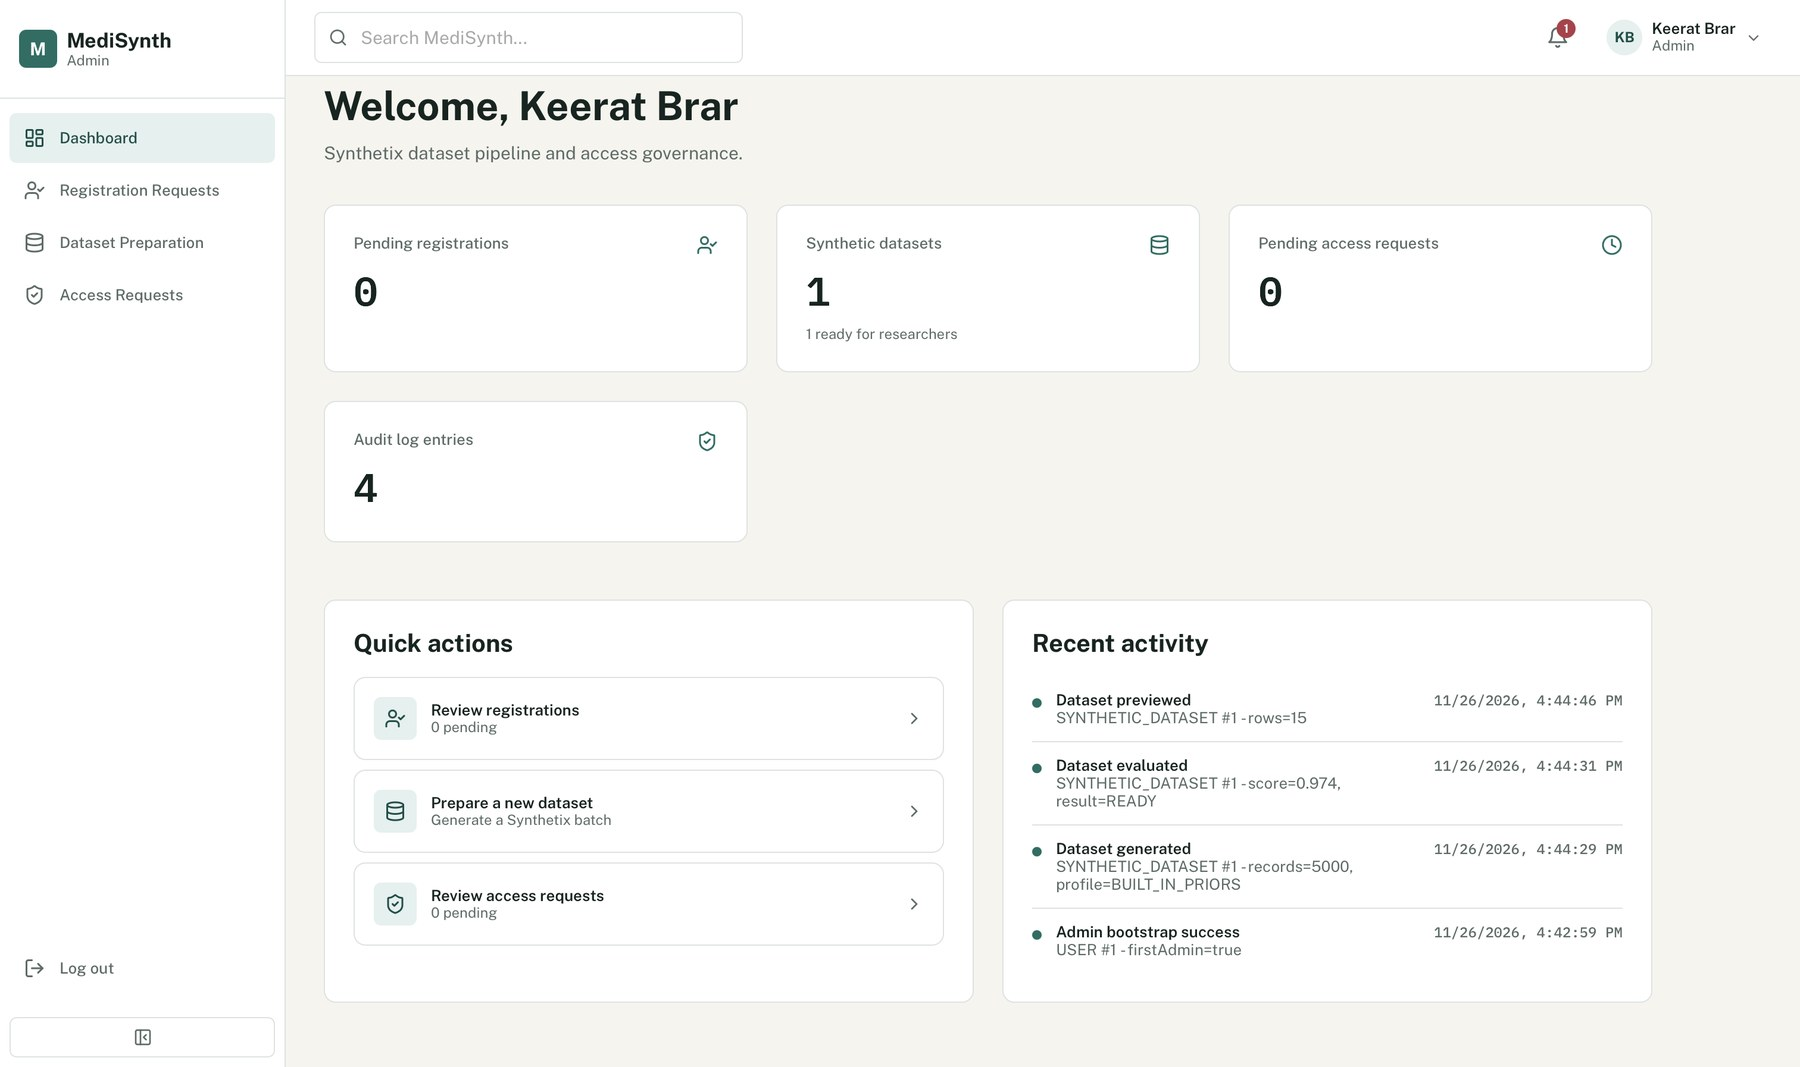
\includegraphics[width=0.95\textwidth,height=0.40\textheight,keepaspectratio]{screenshots/admin_dashboard.jpg}
  \caption{Administrator dashboard: one Synthetix dataset ready for researchers, and recent audit activity (dataset generated with 5,000 records, evaluated with score 0.974 and result READY, then previewed)}
  \label{fig:shot-admin}
\end{figure}

\begin{figure}[H]
  \centering
  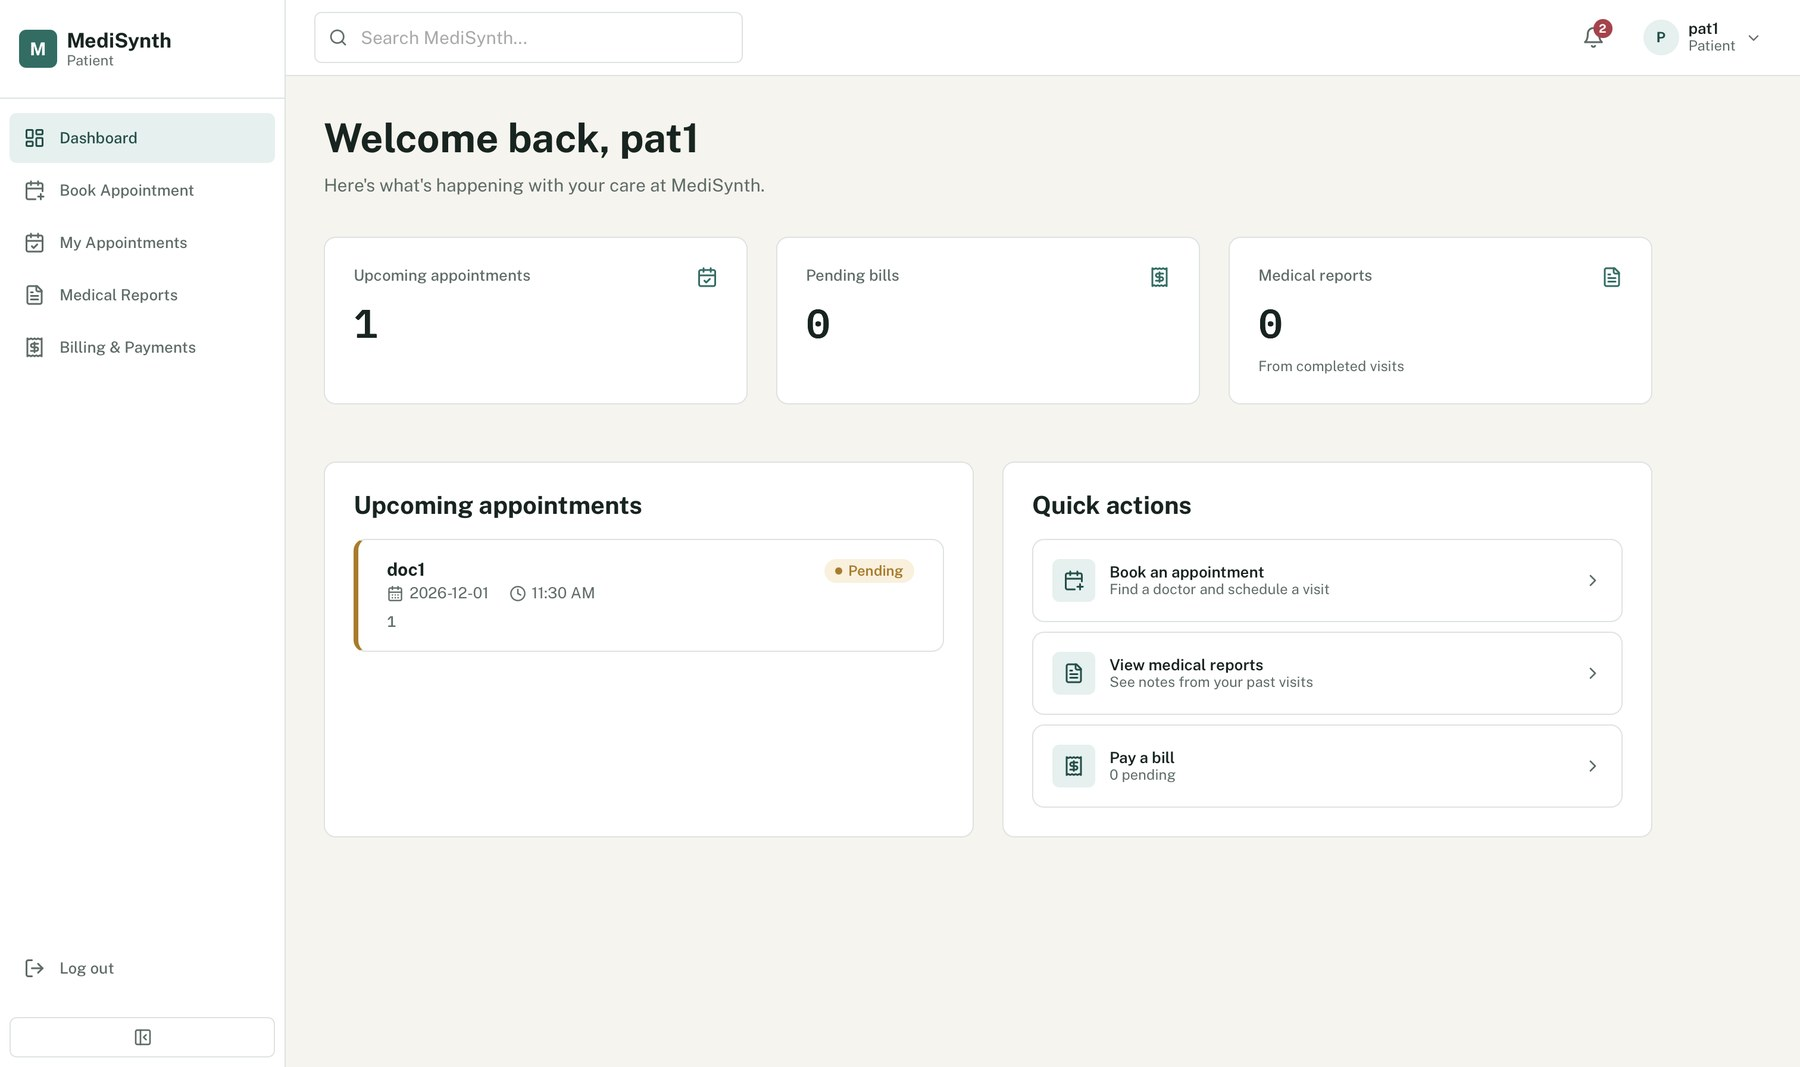
\includegraphics[width=0.95\textwidth,height=0.40\textheight,keepaspectratio]{screenshots/patient_dashboard.jpg}
  \caption{Patient dashboard: the booked appointment with the approved doctor is shown as pending}
  \label{fig:shot-patient}
\end{figure}

\begin{figure}[H]
  \centering
  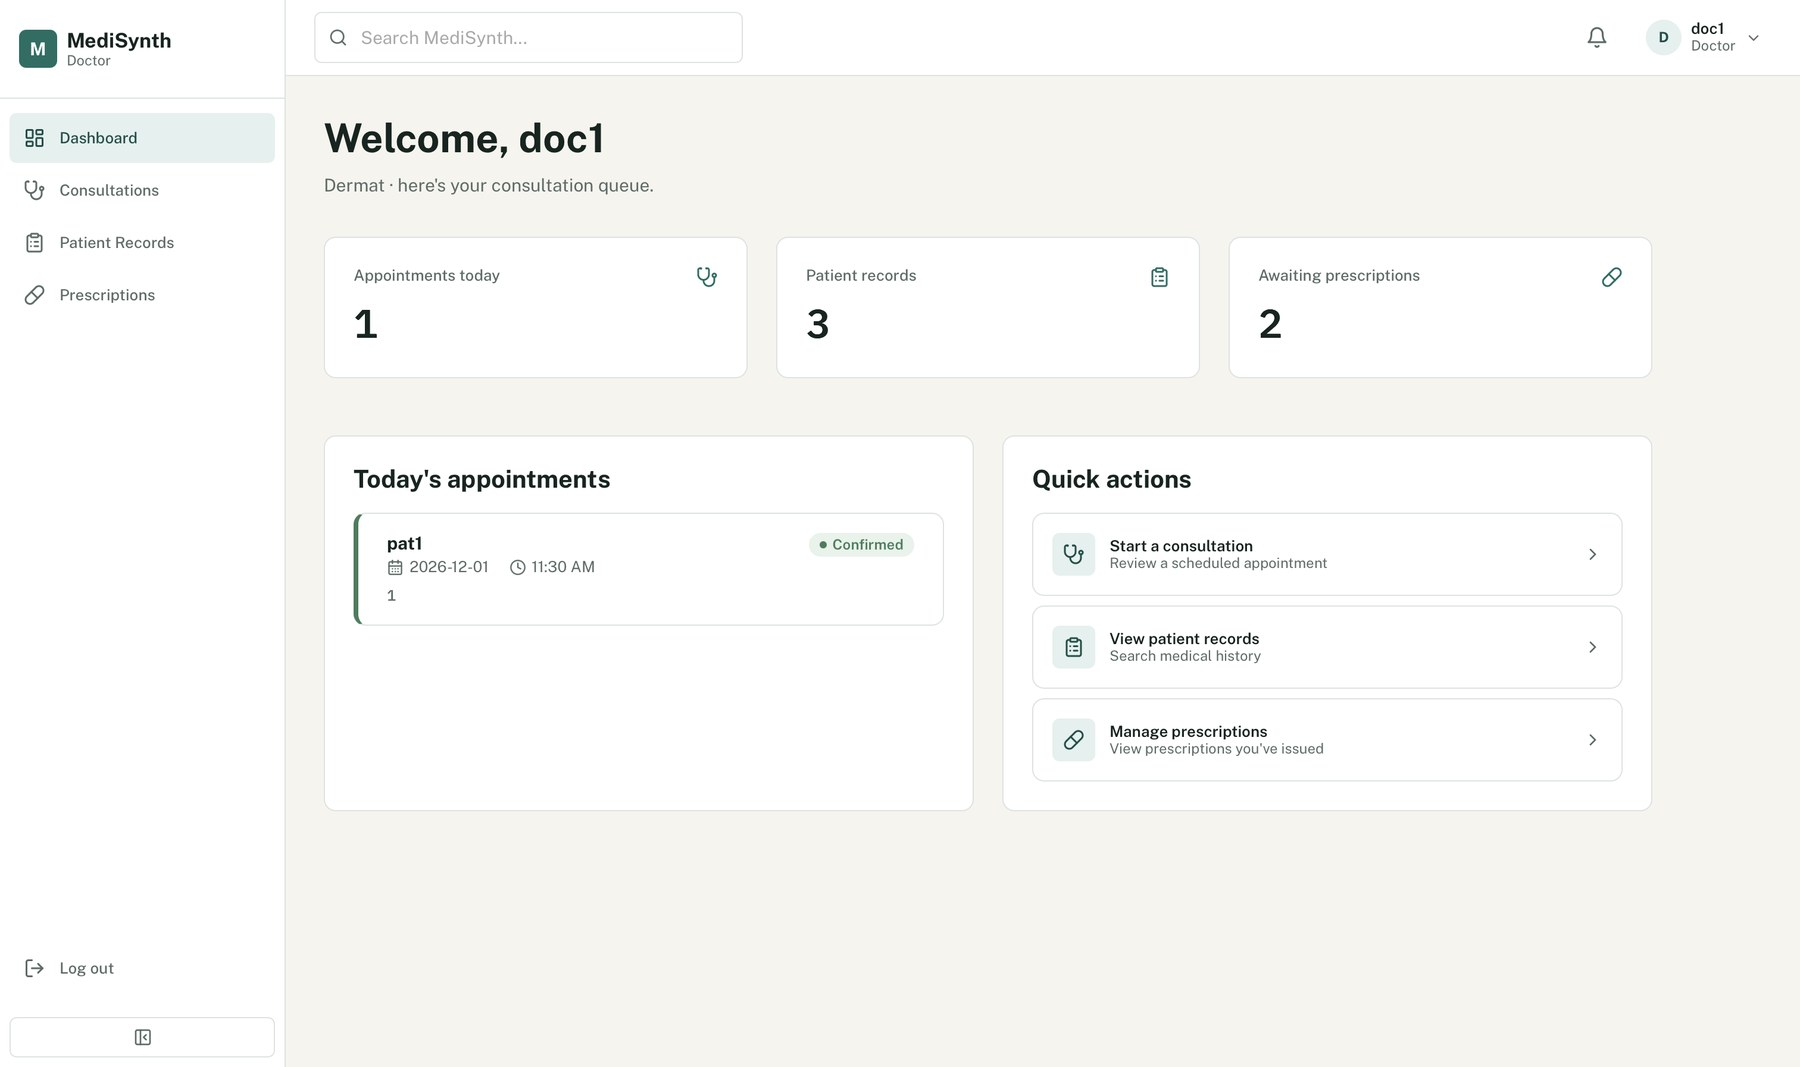
\includegraphics[width=0.95\textwidth,height=0.40\textheight,keepaspectratio]{screenshots/doctor_dashboard.jpg}
  \caption{Doctor dashboard after approval: the same appointment appears in today's queue as confirmed}
  \label{fig:shot-doctor}
\end{figure}

\begin{figure}[H]
  \centering
  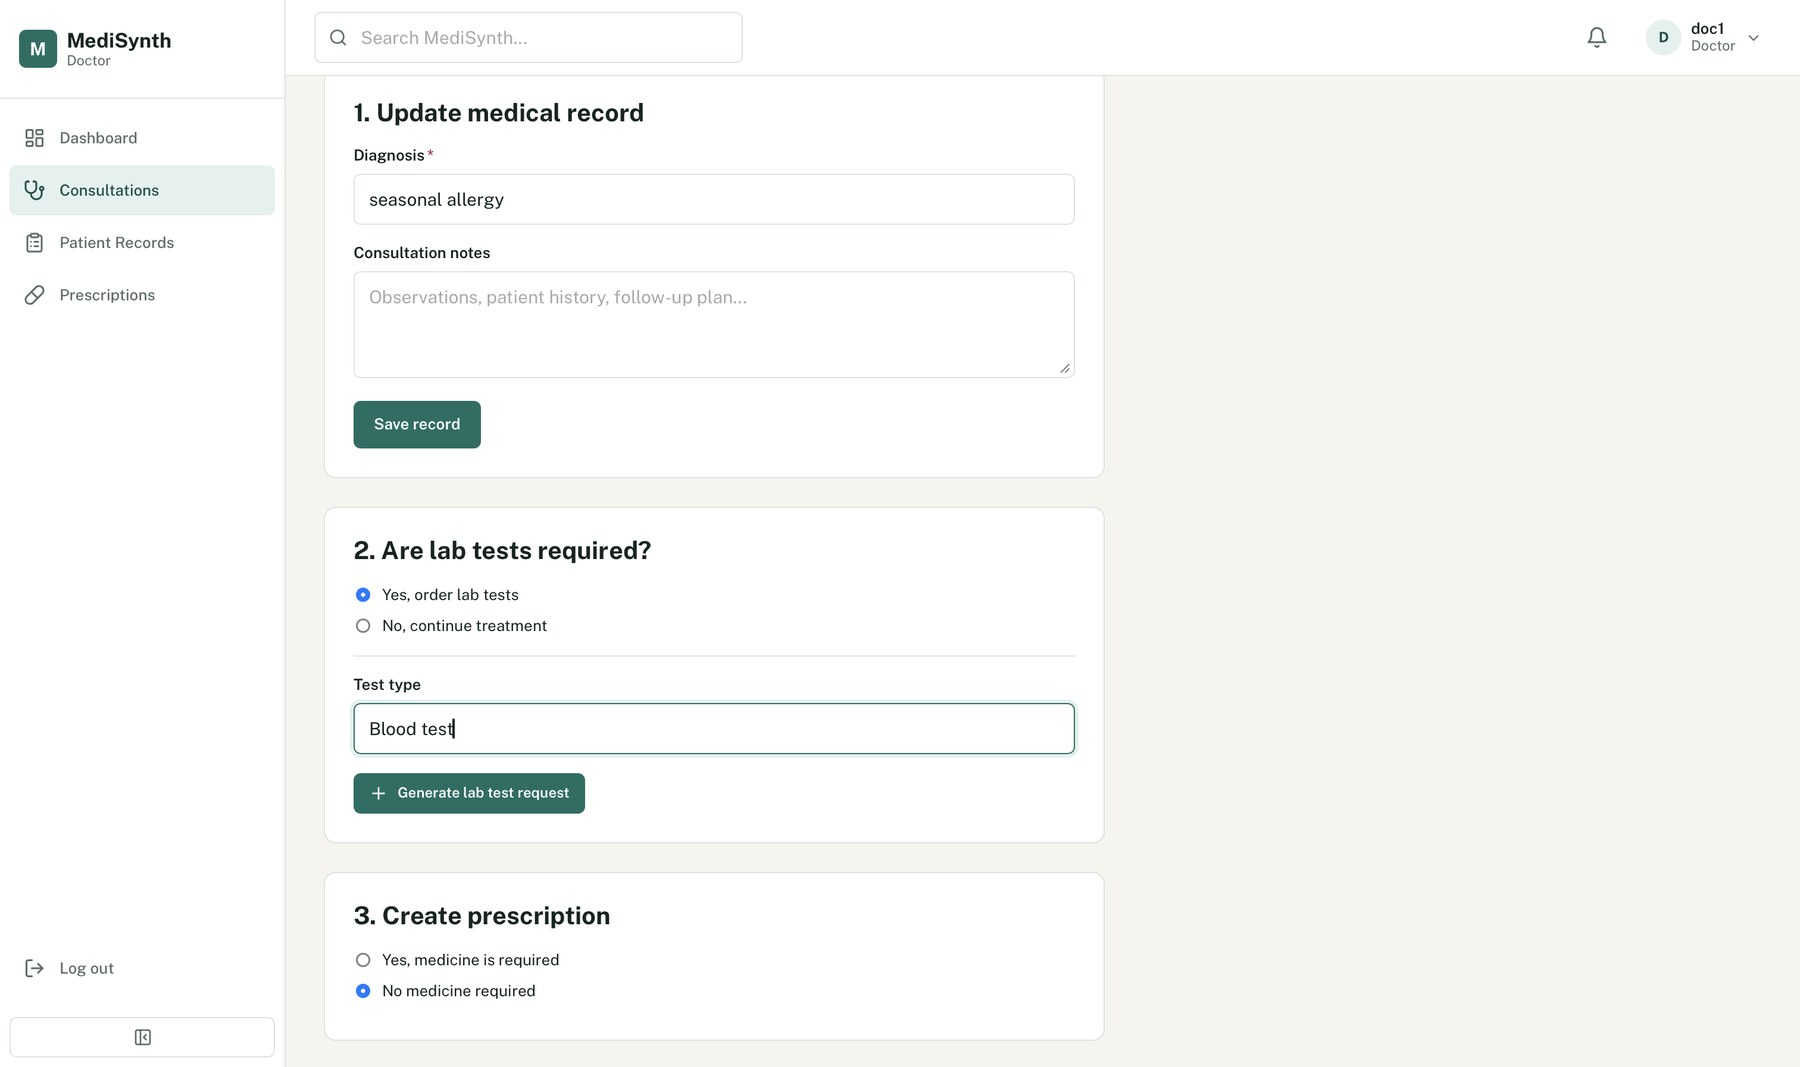
\includegraphics[width=0.95\textwidth,height=0.40\textheight,keepaspectratio]{screenshots/consultation.jpg}
  \caption{Consultation screen: the doctor records a diagnosis and notes and orders a lab test}
  \label{fig:shot-consult}
\end{figure}

Figures~\ref{fig:shot-register} to~\ref{fig:shot-requests} show the approval workflow, Figure~\ref{fig:shot-admin} shows the Synthetix result recorded in the audit log, and Figures~\ref{fig:shot-patient} to~\ref{fig:shot-consult} show the appointment and consultation flow.

\section{Analysis}

\begin{itemize}
  \item \textbf{Objectives met.} The role-based system, the approval
    workflow, appointments, lab tests, the Synthetix engine and the governed
    access workflow are implemented against a real database. Datasets of
    5,000 and 10,000 records pass every gate.
  \item \textbf{Design decision that paid off.} Keeping the engine free of
    framework code allowed it to be calibrated and run on its own. The
    thresholds in Table~\ref{tab:gates} were chosen from those runs, and one
    gate (unique share) was relaxed from 0.5\% to 1\% after 5,000 records
    were found to sit at 0.58\%.
  \item \textbf{Challenges.} The first generator rarely produced chronic
    diagnoses (routine checks were 62\% of patients); raising the chronic
    and acute scores brought the mix to realistic proportions (routine checks
    about 24\%, hypertension about 16\%, type 2 diabetes about 6.5\%).
    Role handling, access to datasets and secret management were designed
    server-side from the start to avoid trusting the client.
\end{itemize}

\section{Limitations}

\begin{itemize}
  \item The generator is a rule-based statistical model, not a machine-learning
    model and not a model of real patients. It learns only the coarse age and
    gender mix of a hospital; its reference distributions and relationship
    thresholds are chosen by the team. It is suitable for demonstrations and
    pipeline testing, not for clinical research conclusions.
  \item $k$-anonymity on three attributes is a basic privacy measure; it does
    not give the formal guarantee of differential privacy, and the evaluator
    does not test attacks such as membership inference.
  \item Prescriptions, pharmacy and billing are not yet connected to the
    backend.
\end{itemize}

% ===== CHAPTER 5: CONCLUSION =====

\chapter{Conclusion}

\section{Summary of Work}

We built MediSynth, a role-based hospital management system with a
Spring Boot and PostgreSQL backend and a React frontend, together with
Synthetix, an in-house synthetic patient data engine with an automatic quality
and privacy evaluator and a governed request--approve--download workflow for
researchers.

\section{Key Findings}

\begin{itemize}
  \item A causal, seeded sampler can reproduce the main age, diagnosis, vital
    sign and laboratory relationships that a hospital system needs for
    realistic testing, without using any individual patient record.
  \item Privacy depends strongly on dataset size: under the same generator,
    500 and 2,000 records fail the $k$-anonymity gate while 5,000 and 10,000
    pass.
  \item Server-side roles, approval before access and per-dataset access
    requests keep sensitive data and actions under administrator control and
    in the audit log.
\end{itemize}

\section{Future Work and Recommendations}

\begin{itemize}
  \item Connect prescriptions, pharmacy and billing to the backend.
  \item Replace or complement the rule-based generator with a learned model
    (for example a Python-based generator) behind the same service interface,
    and add formal privacy measures such as differential privacy.
  \item Add a CI/CD pipeline that builds and tests the backend and frontend
    on every change.
  \item Validate the generator against published public-health statistics for
    the target population.
\end{itemize}

\section{Final Remarks}

MediSynth shows that a team without access to real patient data can still
build and test a realistic hospital system, provided the synthetic data is
generated, checked and shared under clear rules. The engine's limits are
stated openly in this report so that the data is used for what it is: a
privacy-safe stand-in for development and demonstration.

% ===== BIBLIOGRAPHY =====

\begin{thebibliography}{9}
\addcontentsline{toc}{chapter}{Bibliography}
\bibitem{sweeney2000} L.~Sweeney, ``Simple Demographics Often Identify People
  Uniquely,'' Carnegie Mellon University, Data Privacy Working Paper 3, 2000.
\bibitem{sweeney2002} L.~Sweeney, ``k-anonymity: A Model for Protecting
  Privacy,'' \emph{International Journal of Uncertainty, Fuzziness and
  Knowledge-Based Systems}, vol.~10, no.~5, pp.~557--570, 2002.
\bibitem{dpdp} Government of India, \emph{The Digital Personal Data Protection
  Act, 2023}.
\bibitem{hipaa} U.S.\ Department of Health and Human Services, \emph{Health
  Insurance Portability and Accountability Act of 1996 (HIPAA)}.
\bibitem{icd10} World Health Organization, \emph{International Statistical
  Classification of Diseases and Related Health Problems, 10th Revision
  (ICD-10)}.
\end{thebibliography}


% ===== APPENDIX: TEST CASE SHEETS =====
\appendix
\chapter{Test Case Sheets}
The three test-case sheets summarised in Table~\ref{tab:tc} follow, one per test case, in the project template.

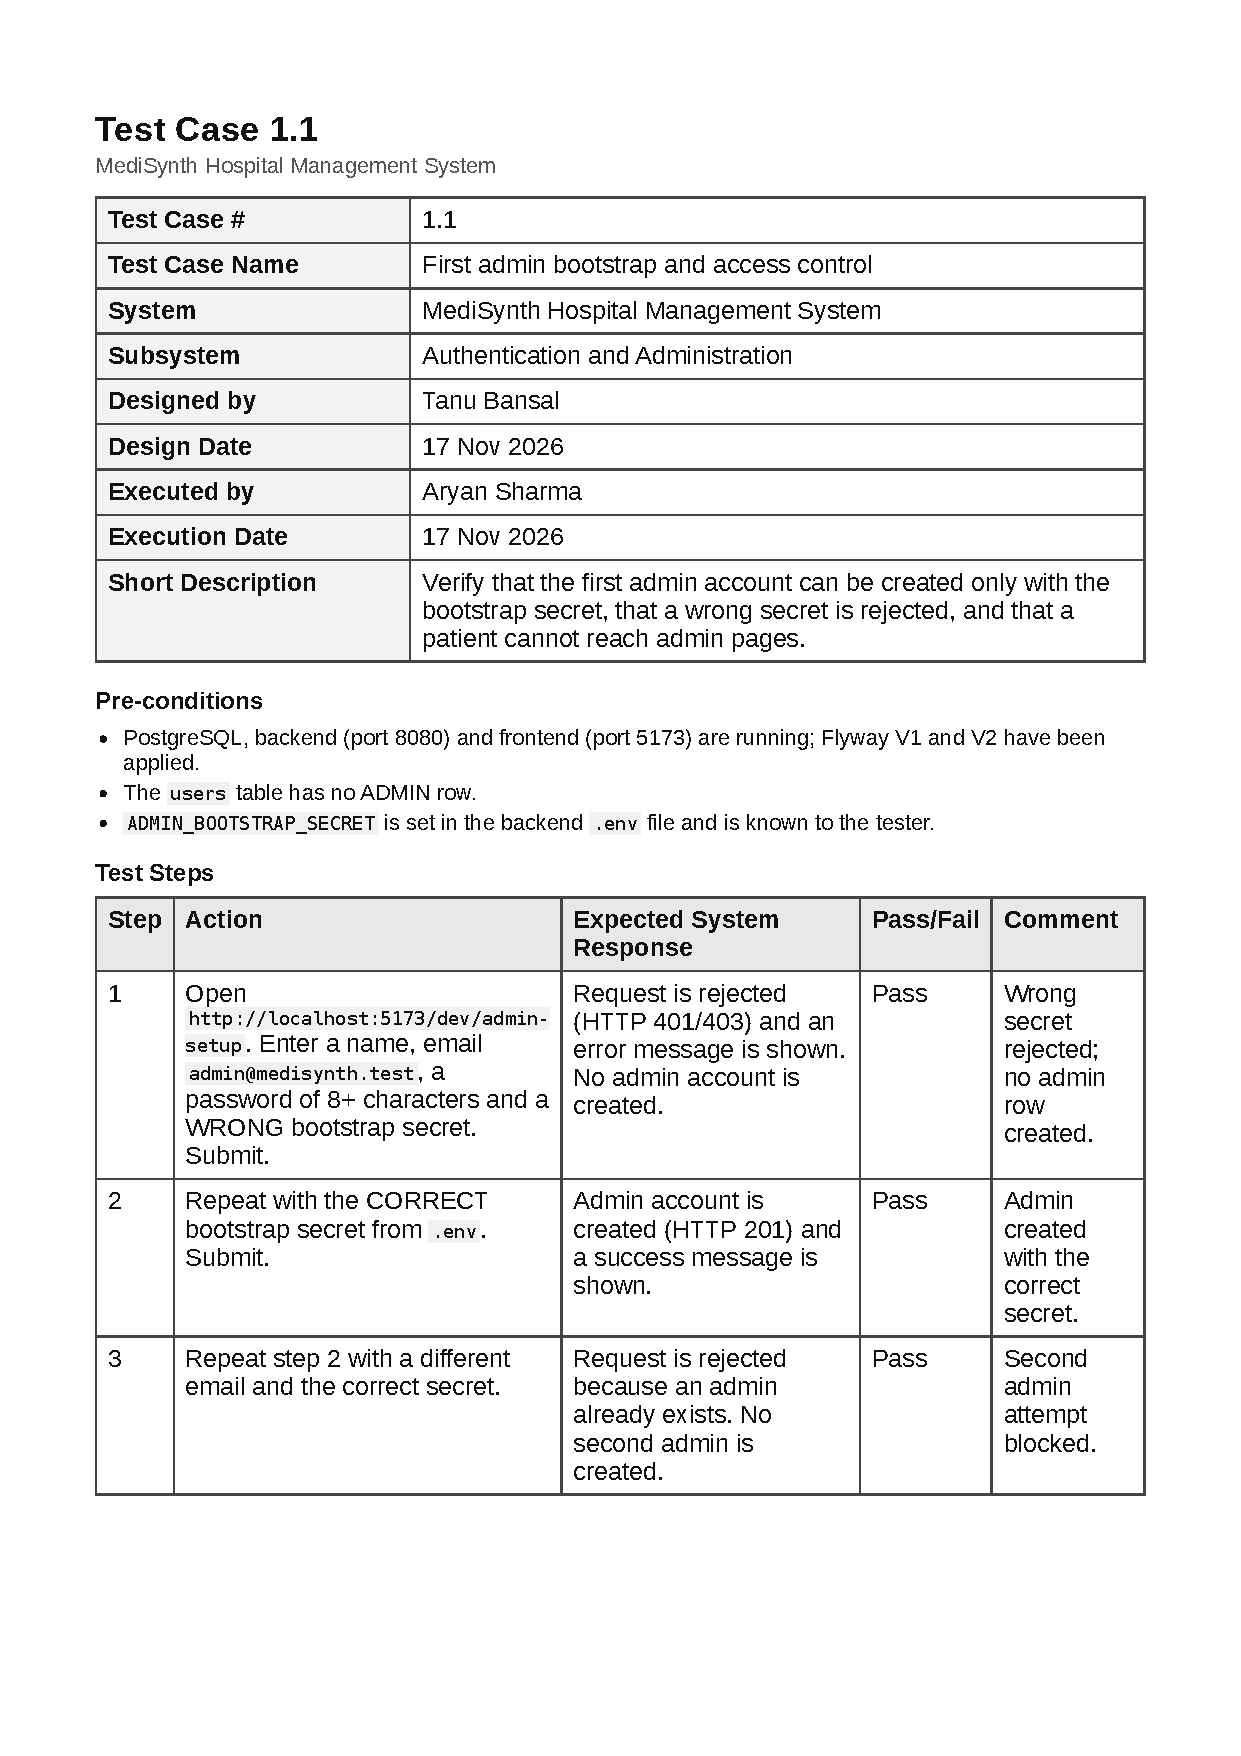
\includepdf[pages=-,scale=0.9,pagecommand={\thispagestyle{plain}}]{testcases/TestCases_All.pdf}

\end{document}
